\documentclass[a4paper]{report}

% --- FONT & NGÔN NGỮ ---
\usepackage{fontspec}
\setmainfont{Times New Roman}
\usepackage[vietnamese]{babel}
\usepackage{microtype} % Tự động tinh chỉnh khoảng cách để giảm lỗi tràn lề

% --- ÉP FONT 13pt TOÀN CỤC ---
\usepackage{fontsize}
\changefontsize[15.6]{13} % Cỡ chữ 13pt, base leading 15.6pt

% --- CANH LỀ CHUẨN A4 KHÓA LUẬN TỐT NGHIỆP TDTU ---
% Lề trái 3.5cm (đóng gáy sách), lề phải 2.0cm, lề trên 3.0cm, lề dưới 3.0cm
\usepackage[top=3.0cm, bottom=3.0cm, left=3.5cm, right=2.0cm, headheight=16pt, headsep=1.0cm, footskip=1.2cm]{geometry}

% --- DÃN DÒNG & THỤT ĐẦU DÒNG ĐOẠN VĂN ---
\usepackage{setspace}
\onehalfspacing % Dãn dòng 1.5 lines chuẩn
\usepackage{indentfirst}
\setlength{\parindent}{1.27cm} % Thụt đầu dòng 1.27cm (0.5 inch)
\setlength{\parskip}{0pt}      % Không dãn cách đoạn thừa thãi
\emergencystretch 3em          % Chống tuyệt đối lỗi tràn lề phải (overfull hbox)

% --- HEADER & FOOTER: ĐÁNH SỐ TRANG GIỮA TRÊN ---
\usepackage{fancyhdr}
\pagestyle{fancy}
\fancyhf{} 
\fancyhead[C]{\fontsize{10pt}{12pt}\selectfont\thepage} % Số trang căn giữa phía trên
\renewcommand{\headrulewidth}{0pt}
\renewcommand{\footrulewidth}{0pt}

% Đảm bảo trang đầu chương / trang plain vẫn có số trang căn giữa phía trên
\fancypagestyle{plain}{
    \fancyhf{} 
    \fancyhead[C]{\fontsize{10pt}{12pt}\selectfont\thepage} 
    \renewcommand{\headrulewidth}{0pt}
}

% --- TOÁN HỌC & HÌNH ẢNH ---
\usepackage{amsmath, amsfonts, amssymb}
\usepackage{graphicx}
\usepackage{tikz}
\usetikzlibrary{calc, positioning}
\usepackage{float}
\usepackage{longtable}
\usepackage{booktabs}
\usepackage{array}
\usepackage{multirow}
\usepackage{tabularx}
\usepackage{xltabular}
\newcolumntype{Y}{>{\centering\arraybackslash}X}
\usepackage{subcaption}
\graphicspath{{media/}}
\usepackage{caption}
\captionsetup{
    font={small},
    labelfont={bf},
    labelsep=colon,
    skip=6pt
}

\usepackage[hidelinks]{hyperref} % Liên kết mục lục sạch sẽ, không viền đỏ

% --- TÙY CHỈNH MỤC LỤC & DANH MỤC (TOC, LOF, LOT) ---
\usepackage{tocloft} 
\renewcommand{\cftdotsep}{0.5} % Dấu chấm mục lục san sát chuẩn Word

% Thêm chữ "CHƯƠNG " vào Mục lục
\renewcommand{\cftchappresnum}{CHƯƠNG } 
\renewcommand{\cftchapaftersnum}{. }    
\setlength{\cftchapnumwidth}{6.0em}     

% 1. Cấp Chương (Chapter): In đậm toàn hàng
\renewcommand{\cftchapfont}{\bfseries}
\renewcommand{\cftchapleader}{\bfseries\cftdotfill{\cftdotsep}}
\renewcommand{\cftchappagefont}{\bfseries}

% 2. Cấp Mục (Section - 1.1): Chữ thường
\renewcommand{\cftsecfont}{\normalfont}
\renewcommand{\cftsecleader}{\normalfont\cftdotfill{\cftdotsep}}
\renewcommand{\cftsecpagefont}{\normalfont}
\setlength{\cftsecnumwidth}{2.2em}

% 3. Cấp Tiểu mục (Subsection - 1.1.1): In nghiêng
\renewcommand{\cftsubsecfont}{\itshape}
\renewcommand{\cftsubsecleader}{\itshape\cftdotfill{\cftdotsep}}
\renewcommand{\cftsubsecpagefont}{\itshape}
\setlength{\cftsubsecnumwidth}{2.8em}

% Khoảng cách giữa các dòng trong Mục lục
\setlength{\cftbeforechapskip}{8pt} 
\setlength{\cftbeforesecskip}{5pt}
\setlength{\cftbeforesubsecskip}{4pt}

% Danh mục hình vẽ
\renewcommand{\cftfigpresnum}{Hình } 
\renewcommand{\cftfigaftersnum}{: }  
\setlength{\cftfignumwidth}{4.5em}   

% Danh mục bảng biểu
\renewcommand{\cfttabpresnum}{Bảng } 
\renewcommand{\cfttabaftersnum}{: }  
\setlength{\cfttabnumwidth}{4.5em}   

% Xóa khoảng trắng thừa giữa các chương trong danh mục hình/bảng
\usepackage{etoolbox}
\makeatletter
\AtBeginDocument{
  \patchcmd{\@chapter}{\addtocontents{lof}{\protect\addvspace{10\p@}}}{}{}{}
  \patchcmd{\@chapter}{\addtocontents{lot}{\protect\addvspace{10\p@}}}{}{}{}
}
\makeatother

% --- ĐỊNH DẠNG TIÊU ĐỀ CÁC CẤP (HEADING SPACING CHUẨN ĐẸP) ---
\usepackage{titlesec}
\setcounter{secnumdepth}{3} % Đánh số tới cấp 1.1.1.1

% Heading 1: Chương (\chapter) - 16pt Bold
\titleformat{\chapter}[hang]
  {\fontsize{16pt}{22pt}\selectfont\bfseries} 
  {CHƯƠNG \thechapter.} 
  {0.5cm} 
  {}
\titlespacing*{\chapter}{0pt}{0pt}{16pt} % Cách dưới 16pt

% Heading 2: Mục lớn (\section) - 14pt Bold, sát lề trái 0cm
\titleformat{\section}[hang]
  {\fontsize{14pt}{19pt}\selectfont\bfseries} 
  {\thesection}
  {0.4cm} 
  {}
\titlespacing*{\section}{0pt}{14pt}{6pt} % Sát lề trái

% Heading 3: Tiểu mục (\subsection - vd 3.1.1) - 13pt Bold Italic, thụt vào 0.635cm (nửa tab)
\titleformat{\subsection}[hang]
  {\fontsize{13pt}{18pt}\selectfont\bfseries\itshape} 
  {\thesubsection}
  {0.35cm} 
  {}
\titlespacing*{\subsection}{0.635cm}{10pt}{4pt} % Thụt vào bậc thang 0.635cm

% Heading 4: Tiểu mục con (\subsubsection - vd 3.1.1.1) - 13pt Italic, thụt vào 1.27cm (1 tab)
\titleformat{\subsubsection}[hang]
  {\fontsize{13pt}{18pt}\selectfont\itshape} 
  {\thesubsubsection}
  {0.3cm} 
  {}
\titlespacing*{\subsubsection}{1.27cm}{8pt}{3pt} % Thụt vào bậc thang 1.27cm

% --- KHOẢNG CÁCH CÔNG THỨC TOÁN HỌC ---
\AtBeginDocument{
  \setlength{\abovedisplayskip}{6pt}
  \setlength{\belowdisplayskip}{6pt}
  \setlength{\abovedisplayshortskip}{3pt} 
  \setlength{\belowdisplayshortskip}{3pt}
}

% --- TÀI LIỆU THAM KHẢO ---
\usepackage{csquotes} 
\DeclareQuoteAlias{english}{vietnamese}

\usepackage[backend=biber, style=ieee]{biblatex}
\addbibresource{backmatter/references.bib}
\usepackage{xurl} 
\let\parencite\cite 



\defbibheading{bibcenter}{
    \clearpage
    \phantomsection
    \addcontentsline{toc}{chapter}{TÀI LIỆU THAM KHẢO}
    \begin{center}
        {\fontsize{16pt}{22pt}\selectfont\bfseries TÀI LIỆU THAM KHẢO\par}
    \end{center}
    \vspace{12pt}
}

\defbibheading{subbib}{
    \noindent #1\par\vspace{6pt}
}

\defbibenvironment{bibliography}
  {\list
     {}
     {\setlength{\leftmargin}{0pt}
      \setlength{\itemindent}{1.27cm}
      \setlength{\itemsep}{0.5\baselineskip}
      \setlength{\parsep}{0pt}}}
  {\endlist}
  {\item}



% --- TÙY CHỈNH DANH SÁCH (ITEMIZE / ENUMERATE) ---
\usepackage{enumitem}
\setlist{
    topsep=3pt,
    partopsep=0pt,
    itemsep=2pt,
    parsep=0pt,
    labelindent=1.27cm,
    leftmargin=*,
    align=left,
    labelsep=0.4cm
}
\renewcommand{\labelitemi}{--}
\renewcommand{\labelitemii}{$-$}
% --- Lệnh đánh dấu chỗ cần điền số liệu thật, dùng thuần LaTeX (không cần gói ngoài) ---
% XOÁ lệnh \todo{...} này và thay bằng nội dung thật trước khi nộp báo cáo.
\newcommand{\todo}[1]{\textbf{[TODO: #1]}}


\begin{document}
    % --- TRANG BÌA ---
    % --- TRANG BÌA CHÍNH ---
\begin{titlepage}
\begin{center}
{\fontsize{14pt}{16.8pt}\selectfont TỔNG LIÊN ĐOÀN LAO ĐỘNG VIỆT NAM\par}
{\fontsize{14pt}{16.8pt}\selectfont \textbf{TRƯỜNG ĐẠI HỌC TÔN ĐỨC THẮNG}\par}
{\fontsize{14pt}{16.8pt}\selectfont \textbf{KHOA CÔNG NGHỆ THÔNG TIN}\par}

\vspace{0.8cm}

\includegraphics[trim=0pt 0pt 5pt 0pt, clip, width=4.13cm, height=2.29cm]{media/logo.png}
\vspace{1.0cm}

{\fontsize{13pt}{16pt}\selectfont \textbf{LÊ MINH LÝ - 52300220}\par}
\vspace{0.1cm}
{\fontsize{13pt}{16pt}\selectfont \textbf{SỬ THỊ YẾN LINH - 52300218}\par}

\vspace{1.5cm}
{\fontsize{16pt}{20pt}\selectfont \textbf{XÂY DỰNG MÔ HÌNH KHUYẾN NGHỊ LAI\\KẾT HỢP NHÂN TỬ HOÁ MA TRẬN\\VÀ MẠNG LƯỚI THẦN KINH SÂU}\par}

\vspace{1.8cm}
{\fontsize{16pt}{20pt}\selectfont \textbf{DỰ ÁN CÔNG NGHỆ THÔNG TIN}\par}
\vspace{0.4cm}
{\fontsize{16pt}{20pt}\selectfont \textbf{MẠNG MÁY TÍNH VÀ TRUYỀN THÔNG\\DỮ LIỆU}\par}

\vfill
{\fontsize{13pt}{16pt}\selectfont \textbf{THÀNH PHỐ HỒ CHÍ MINH, NĂM 2026}\par}
\end{center}
\end{titlepage}

% --- TRANG PHỤ BÌA ---
\newpage
\begin{titlepage}
\begin{center}
{\fontsize{14pt}{16.8pt}\selectfont TỔNG LIÊN ĐOÀN LAO ĐỘNG VIỆT NAM\par}
{\fontsize{14pt}{16.8pt}\selectfont \textbf{TRƯỜNG ĐẠI HỌC TÔN ĐỨC THẮNG}\par}
{\fontsize{14pt}{16.8pt}\selectfont \textbf{KHOA CÔNG NGHỆ THÔNG TIN}\par}

\vspace{0.8cm}

\includegraphics[trim=0pt 0pt 5pt 0pt, clip, width=4.13cm, height=2.29cm]{media/logo.png}
\vspace{0.8cm}

{\fontsize{13pt}{16pt}\selectfont \textbf{LÊ MINH LÝ - 52300220}\par}
\vspace{0.1cm}
{\fontsize{13pt}{16pt}\selectfont \textbf{SỬ THỊ YẾN LINH - 52300218}\par}

\vspace{1.0cm}
{\fontsize{16pt}{20pt}\selectfont \textbf{XÂY DỰNG MÔ HÌNH KHUYẾN NGHỊ LAI\\KẾT HỢP NHÂN TỬ HOÁ MA TRẬN\\VÀ MẠNG LƯỚI THẦN KINH SÂU}\par}

\vspace{1.2cm}
{\fontsize{16pt}{20pt}\selectfont \textbf{DỰ ÁN CÔNG NGHỆ THÔNG TIN}\par}
\vspace{0.3cm}
{\fontsize{16pt}{20pt}\selectfont \textbf{MẠNG MÁY TÍNH VÀ TRUYỀN THÔNG\\DỮ LIỆU}\par}

\vspace{1.0cm}
{\fontsize{13pt}{16pt}\selectfont Giảng viên hướng dẫn\par}
\vspace{0.1cm}
{\fontsize{14pt}{17pt}\selectfont \textbf{TS. HỒ THỊ LINH}\par}

\vfill
{\fontsize{13pt}{16pt}\selectfont \textbf{THÀNH PHỐ HỒ CHÍ MINH, NĂM 2026}\par}
\end{center}
\end{titlepage}

    % --- PHẦN MỞ ĐẦU ---
    \pagenumbering{roman}
    \pagestyle{fancy}
    \setcounter{page}{1}
    
    \newpage
\begin{center}
{\fontsize{16pt}{19.2pt}\selectfont \textbf{LỜI CẢM ƠN}\par}
\end{center}
\vspace{0.5cm}

Lời đầu tiên, chúng em xin được bày tỏ lòng biết ơn chân thành và sâu sắc nhất đến TS. Hồ Thị Linh – người Cô đã luôn tận tình hướng dẫn, dành nhiều tâm huyết và đồng hành cùng chúng em trong suốt quá trình thực hiện dự án này. Những lời khuyên định hướng quý báu, sự chỉ dẫn ân cần và nguồn động viên to lớn của Cô chính là điểm tựa vững chắc giúp chúng em vượt qua những khó khăn để hoàn thành đề tài một cách tốt nhất.

Chúng em cũng xin gửi lời tri ân sâu sắc đến Ban giám hiệu cùng toàn thể quý Thầy Cô trường Đại học Tôn Đức Thắng, đặc biệt là các Thầy Cô thuộc Khoa Công nghệ Thông tin, những người đã truyền dạy cho chúng em nền tảng kiến thức chuyên môn vững chắc và rèn luyện kỹ năng thực tiễn trong suốt những năm học tập dưới mái trường.

Dù đã dành nhiều tâm huyết và nỗ lực hoàn thiện dự án một cách chỉn chu nhất, song do giới hạn về kiến thức và kinh nghiệm thực tiễn, báo cáo chắc chắn không tránh khỏi những thiếu sót ngoài ý muốn. Chúng em rất mong nhận được sự cảm thông cùng những ý kiến đóng góp, chỉ bảo quý báu từ quý Thầy Cô trong Hội đồng chấm dự án để đề tài được hoàn thiện hơn.

Chúng em xin kính chúc quý Thầy Cô luôn dồi dào sức khỏe, hạnh phúc và gặt hái được nhiều thành công hơn nữa trong sự nghiệp cao quý của mình!

Chúng em xin chân thành cảm ơn!

\vspace{0.8cm}

\begin{flushright}
\textit{TP. Hồ Chí Minh, ngày 09 tháng 05 năm 2026}
\end{flushright}

\vspace{0.3cm}
\noindent
\begin{minipage}[t]{0.48\textwidth}
    \centering
    \textbf{Tác giả} \\
    \textit{(Ký và ghi rõ họ tên)} \\
    \vspace{2.5cm}
    \textbf{Lê Minh Lý}
\end{minipage}
\hfill
\begin{minipage}[t]{0.48\textwidth}
    \centering
    \textbf{Tác giả} \\
    \textit{(Ký và ghi rõ họ tên)} \\
    \vspace{2.5cm}
    \textbf{Sử Thị Yến Linh}
\end{minipage}
    \newpage
    \newpage
\begin{center}
{\fontsize{16pt}{19.2pt}\selectfont \textbf{CÔNG TRÌNH ĐƯỢC HOÀN THÀNH \\TẠI TRƯỜNG ĐẠI HỌC TÔN ĐỨC THẮNG}\par}
\end{center}
\vspace{0.5cm}

Chúng tôi xin cam đoan báo cáo dự án này là công trình nghiên cứu độc lập của chúng tôi dưới sự hướng dẫn khoa học trực tiếp của TS. Hồ Thị Linh. Mọi số liệu, quá trình phân tích và kết quả thực nghiệm trình bày trong báo cáo là hoàn toàn trung thực, khách quan và chưa từng được công bố dưới bất kỳ hình thức nào trước đây.

Các nguồn tài liệu tham khảo, số liệu trích dẫn phục vụ cho dự án đều có nguồn gốc rõ ràng, có độ tin cậy cao và được chú thích đầy đủ trong danh mục tài liệu tham khảo. 

Chúng tôi xin hoàn toàn chịu trách nhiệm trước Nhà trường và pháp luật về tính chân thực, bản quyền cũng như các vi phạm quyền sở hữu trí tuệ liên quan đến nội dung báo cáo dự án này.

\vspace{0.5cm}
\begin{flushright}
\textit{TP. Hồ Chí Minh, ngày \todo{[điền ngày nộp thật]}}
\end{flushright}

\vspace{0.3cm}
\noindent
\begin{minipage}[t]{0.48\textwidth}
    \centering
    \textbf{Tác giả} \\
    \textit{(Ký và ghi rõ họ tên)} \\
    \vspace{3cm}
    \textbf{Lê Minh Lý}
\end{minipage}
\hfill
\begin{minipage}[t]{0.48\textwidth}
    \centering
    \textbf{Tác giả} \\
    \textit{(Ký và ghi rõ họ tên)} \\
    \vspace{3cm}
    \textbf{Sử Thị Yến Linh}
\end{minipage}
    % % frontmatter/declaration.tex
\cleardoublepage % Đảm bảo sang trang mới
\pagestyle{empty} % Không hiện số trang

\begin{center}
    \textbf{\Large THESIS PLEDGE}
\end{center}
\addcontentsline{toc}{section}{THESIS PLEDGE}

\vspace{0.5cm}



This thesis was carried out at Ton Duc Thang University.

Advisor: PhD. Ho Thi Linh

\vspace{0.2cm}

This thesis is defended at the Undergraduate Thesis Examination Committee was held at Ton Duc Thang University on … / … / ……

Confirmation of the Chairman of the Undergraduate Thesis Examination Committee and the Dean of the faculty after receiving the modified thesis (if any).

\vspace{2cm}

\begin{center}
\begin{tabular}{cc}
    \begin{minipage}{0.45\textwidth}
        \centering
        \textbf{CHAIRMAN}\\[2cm]
        ...........................................
    \end{minipage}
    &
    \begin{minipage}{0.45\textwidth}
        \centering
        \textbf{DEAN OF FACULTY}\\[2cm]
        ...........................................
    \end{minipage}
\end{tabular}
\end{center}
    \newpage
\begin{center}
    \textbf{\fontsize{16pt}{24pt}\selectfont PHẦN XÁC NHẬN VÀ ĐÁNH GIÁ CỦA GIẢNG VIÊN}
\end{center}

\vspace{0.5cm}

% --- PHẦN 1: GV HƯỚNG DẪN ---
\noindent \textbf{Phần xác nhận của GV hướng dẫn} \\
\rule{\textwidth}{0.4pt} \\ 
\rule{\textwidth}{0.4pt} \\
\rule{\textwidth}{0.4pt} \\ 
\rule{\textwidth}{0.4pt} \\ 
\rule{\textwidth}{0.4pt} \\ 
\rule{0.7\textwidth}{0.4pt} % Dòng kẻ ngắn cuối cùng

\vspace{0.3cm}
\begin{flushright}
    \begin{minipage}{0.5\textwidth}
        \centering
        Tp. Hồ Chí Minh, ngày \dots\dots tháng \dots\dots năm \dots\dots \\
        (Ký và ghi họ tên)
        \vspace{2.5cm} % Khoảng trống để GV ký
    \end{minipage}
\end{flushright}


% --- PHẦN 2: GV CHẤM BÀI ---
\noindent \textbf{Phần đánh giá của GV chấm bài} \\
\rule{\textwidth}{0.4pt} \\
\rule{\textwidth}{0.4pt} \\ 
\rule{\textwidth}{0.4pt} \\ 
\rule{\textwidth}{0.4pt} \\
\rule{\textwidth}{0.4pt} \\ 
\rule{0.7\textwidth}{0.4pt}

\vspace{0.3cm}
\begin{flushright}
    \begin{minipage}{0.5\textwidth}
        \centering
        Tp. Hồ Chí Minh, ngày \dots\dots tháng \dots\dots năm \dots\dots \\
        (Ký và ghi họ tên)
        \vspace{2.5cm}
    \end{minipage}
\end{flushright}
    \newpage
\begin{center}
{\fontsize{15pt}{18pt}\selectfont \textbf{XÂY DỰNG MÔ HÌNH KHUYẾN NGHỊ LAI KẾT HỢP NHÂN TỬ HOÁ MA TRẬN VÀ MẠNG LƯỚI THẦN KINH SÂU}\par}
\vspace{0.5cm}
{\fontsize{16pt}{19.2pt}\selectfont \textbf{TÓM TẮT}\par}
\end{center}
\vspace{0.2cm}

Trong kỷ nguyên thương mại điện tử và kinh tế số, hệ thống gợi ý (Recommendation System) đóng vai trò then chốt trong việc tối ưu hóa trải nghiệm người dùng và nâng cao doanh thu doanh nghiệp. Các phương pháp Lọc cộng tác (Collaborative Filtering -- CF) truyền thống như Nhân tử hóa ma trận (Matrix Factorization -- MF) chủ yếu sử dụng tích vô hướng để mô hình hóa tương tác giữa người dùng và sản phẩm \parencite{koren2009matrix}. Tuy nhiên, việc phụ thuộc vào tuyến tính hóa khiến MF khó nắm bắt được các mối quan hệ phức tạp và phi tuyến trong không gian đặc trưng ẩn \parencite{he2017ncf}.

Dự án tập trung nghiên cứu và xây dựng mô hình khuyến nghị lai Neural Matrix Factorization (NeuMF) kết hợp giữa Generalized Matrix Factorization (GMF) và Multi-Layer Perceptron (MLP) \parencite{he2017ncf}. Mô hình tận dụng ưu thế tuyến tính của GMF cùng khả năng học các mối liên hệ phi tuyến sâu của MLP để nâng cao độ chính xác trong việc dự đoán hành vi tương tác dựa trên tín hiệu phản hồi ẩn (Implicit Feedback).

Nghiên cứu được triển khai thực nghiệm trên hai bộ dữ liệu độc lập có đặc trưng cấu trúc khác biệt rõ rệt: DataCo Smart Supply Chain \parencite{dataco2019} (catalog nhỏ, dày đặc) và H\&M Personalized Fashion Recommendations (catalog lớn, cực thưa; tệp giao dịch gốc 31,8 triệu dòng được xử lý bằng một cơ chế cache Parquet gọn nhẹ, cho phép xử lý trên phần cứng CPU phổ thông). Quy trình xử lý dữ liệu xây dựng ma trận tương tác User--Item dạng phản hồi ẩn kết hợp trọng số giá trị đơn hàng, áp dụng kỹ thuật lấy mẫu tiêu cực (Negative Sampling) và phương pháp đánh giá Leave-One-Out theo thời gian. Kết quả kiểm chứng định lượng qua các chỉ số HR@K, NDCG@K \parencite{jarvelin2002} theo cả hai giao thức Full Ranking và Sampled-99 cho thấy NeuMF vượt trội các baseline cổ điển (Random, Most Popular, ItemKNN, BPR-MF) trên cả hai bộ dữ liệu, nhưng chưa cho thấy cải thiện rõ rệt so với chính các nhánh thành phần của nó (GMF, MLP) khi đứng riêng. Đáng chú ý, phân tích bóc tách thành phần (Ablation Study) đối chiếu Early Fusion và NeuMF (Late Fusion) cho kết quả trái ngược nhau giữa hai bộ dữ liệu -- cho thấy thời điểm hợp nhất biểu diễn tối ưu phụ thuộc vào mật độ/quy mô catalog chứ không phải một lựa chọn kiến trúc cố định. Nghiên cứu cũng thực hiện đánh giá phân tầng theo độ phổ biến (Popular/Long-tail), phát hiện dấu hiệu thiên vị phổ biến rõ rệt ở nhiều mô hình, trong phạm vi nhóm người dùng/sản phẩm đã có đủ lịch sử tương tác; kiểm định ý nghĩa thống kê đa seed được xác định là bước kiểm chứng cần thiết tiếp theo.
    \newpage
\begin{center}
{\fontsize{15pt}{18pt}\selectfont \textbf{BUILDING A HYBRID RECOMMENDATION MODEL COMBINING MATRIX FACTORIZATION AND DEEP NEURAL NETWORKS}\par}
\vspace{0.5cm}
{\fontsize{16pt}{19.2pt}\selectfont \textbf{ABSTRACT}\par}
\end{center}
\vspace{0.2cm}

In the era of e-commerce and the digital economy, recommendation systems play a pivotal role in optimizing user experience and driving business revenue. Traditional Collaborative Filtering approaches such as Matrix Factorization primarily rely on the inner product to model user--item interactions \parencite{koren2009matrix}, which restricts them from capturing complex, non-linear relationships \parencite{he2017ncf}.

This project focuses on designing and building a hybrid Neural Matrix Factorization (NeuMF) recommendation model that integrates Generalized Matrix Factorization (GMF) and Multi-Layer Perceptron (MLP) \parencite{he2017ncf}. The architecture leverages the linear capability of GMF alongside the deep non-linear learning power of MLP to enhance prediction accuracy based on implicit feedback signals.

The empirical evaluation is conducted on two independent datasets with markedly different structural characteristics: DataCo Smart Supply Chain \parencite{dataco2019} (small, dense catalog) and H\&M Personalized Fashion Recommendations (large, extremely sparse catalog; the original 31.8-million-row transaction file is processed through a lightweight Parquet caching mechanism that makes it tractable on commodity CPU hardware). The data pipeline constructs a User--Item interaction matrix with weighted implicit feedback based on order value, implements Negative Sampling techniques, and applies a temporal Leave-One-Out evaluation protocol. Quantitative results evaluated via HR@K and NDCG@K \parencite{jarvelin2002} under both the Full Ranking and Sampled-99 protocols show that NeuMF clearly outperforms classical baselines (Random, Most Popular, ItemKNN, BPR-MF) on both datasets, but does not show a clear improvement over its own standalone components (GMF, MLP). Notably, the ablation analysis comparing Early Fusion and NeuMF (Late Fusion) yields opposite outcomes across the two datasets -- indicating that the optimal fusion timing depends on catalog density/scale rather than being a fixed architectural choice. The study also presents a Popular/Long-tail stratified evaluation, revealing pronounced popularity bias in several models, within the scope of users and items with sufficient interaction history; multi-seed statistical significance testing is identified as a necessary next validation step.
    \newpage
% --- MỤC LỤC ---
\begin{center}
{\fontsize{16pt}{19.2pt}\selectfont \textbf{MỤC LỤC}\par}
\end{center}
\vspace{0.5cm}
\makeatletter
\@starttoc{toc}
\makeatother
\clearpage

% --- DANH MỤC HÌNH VẼ ---
\phantomsection
\addcontentsline{toc}{chapter}{DANH MỤC HÌNH VẼ}
\begin{center}
{\fontsize{16pt}{19.2pt}\selectfont \textbf{DANH MỤC HÌNH VẼ}\par}
\end{center}
\vspace{0.5cm}
\makeatletter
\@starttoc{lof}
\makeatother
\clearpage

% --- DANH MỤC BẢNG BIỂU ---
\phantomsection
\addcontentsline{toc}{chapter}{DANH MỤC BẢNG BIỂU}
\begin{center}
{\fontsize{16pt}{19.2pt}\selectfont \textbf{DANH MỤC BẢNG BIỂU}\par}
\end{center}
\vspace{0.5cm}
\makeatletter
\@starttoc{lot}
\makeatother
\clearpage

% --- DANH MỤC CÁC CHỮ VIẾT TẮT ---
\phantomsection
\addcontentsline{toc}{chapter}{DANH MỤC CÁC CHỮ VIẾT TẮT}
\begin{center}
{\fontsize{16pt}{19.2pt}\selectfont \textbf{DANH MỤC CÁC CHỮ VIẾT TẮT}\par}
\end{center}
\vspace{0.5cm}

{
\renewcommand{\arraystretch}{1.4} 
\noindent
\begin{tabular}{p{2.5cm} p{11.5cm}}
ALS & Alternating Least Squares (Bình phương tối thiểu luân phiên) \\
BCE & Binary Cross-Entropy (Entropy chéo nhị phân) \\
BPR & Bayesian Personalized Ranking (Xếp hạng cá nhân hóa Bayes) \\
CF & Collaborative Filtering (Lọc cộng tác) \\
DCG & Discounted Cumulative Gain (Mức tăng tích lũy chiết khấu) \\
DL & Deep Learning (Học sâu) \\
GMF & Generalized Matrix Factorization (Nhân tử hóa ma trận tổng quát) \\
GPU & Graphics Processing Unit (Bộ xử lý đồ họa) \\
HR & Hit Ratio (Tỷ lệ đánh trúng) \\
IDCG & Ideal Discounted Cumulative Gain (Mức tăng tích lũy chiết khấu lý tưởng) \\
MF & Matrix Factorization (Nhân tử hóa ma trận) \\
MLP & Multi-Layer Perceptron (Mạng nơ-ron truyền thẳng đa tầng) \\
NCF & Neural Collaborative Filtering (Lọc cộng tác dựa trên nơ-ron) \\
NDCG & Normalized Discounted Cumulative Gain (Mức tăng tích lũy chiết khấu chuẩn hóa) \\
NeuMF & Neural Matrix Factorization (Nhân tử hóa ma trận thần kinh) \\
ReLU & Rectified Linear Unit (Đơn vị chỉnh lưu tuyến tính) \\
SGD & Stochastic Gradient Descent (Hạ độ dốc ngẫu nhiên) \\
SVD & Singular Value Decomposition (Phân rã giá trị kỳ dị) \\
\end{tabular}
} 
\clearpage
    \clearpage

    % --- PHẦN NỘI DUNG CHÍNH ---
    \pagenumbering{arabic}
    \pagestyle{fancy}
    \chapter{TỔNG QUAN VỀ ĐỀ TÀI}
\label{chap:tongquan}

\section{Bối cảnh nghiên cứu và tính cấp thiết của đề tài}
\label{sec:boicanh}

\subsection{Quan sát ban đầu từ dữ liệu và động lực chọn đề tài}
\label{subsec:thuctrang}

Động lực trực tiếp của đề tài xuất phát từ việc khảo sát bộ dữ liệu DataCo Smart Supply Chain \parencite{dataco2019} trước khi bắt tay vào xây dựng mô hình: tệp giao dịch gốc ghi nhận 180.519 dòng nhưng chỉ liên quan đến 118 mã sản phẩm phân biệt (mục~\ref{subsec:dataco_description}), tức mỗi sản phẩm trung bình xuất hiện trong hàng nghìn giao dịch của hàng nghìn khách hàng khác nhau. Cấu trúc dữ liệu "nhiều User -- ít Item -- lặp lại tương tác dày đặc" này khác hẳn với kịch bản phim ảnh (MovieLens) hay mạng ảnh (Pinterest) mà phần lớn tài liệu về NCF/NeuMF gốc \parencite{he2017ncf} sử dụng để kiểm chứng -- đặt ra câu hỏi cụ thể mà nhóm muốn trả lời qua đề tài: một kiến trúc lai tuyến tính--phi tuyến như NeuMF có còn phát huy ưu thế trên một catalog nhỏ, dày đặc và mang tính chuỗi cung ứng thực tế hay không, hay lợi ích của nó chỉ rõ ràng trên các catalog lớn hơn. Để trả lời câu hỏi này một cách khách quan hơn (không chỉ dựa vào một bộ dữ liệu duy nhất), nhóm bổ sung thêm bộ dữ liệu đối chứng H\&M Personalized Fashion Recommendations có cấu trúc gần như ngược lại (catalog lớn, cực thưa, mục~\ref{sec:hm_pipeline}) làm phép kiểm tra chéo cho các kết luận rút ra.

Ở góc độ ứng dụng, việc cá nhân hóa gợi ý sản phẩm trong bối cảnh thương mại điện tử/chuỗi cung ứng vẫn giữ nguyên giá trị đã được ghi nhận trong tài liệu học thuật -- giảm chi phí tìm kiếm của khách hàng và hỗ trợ dự báo nhu cầu tiêu thụ cho doanh nghiệp \parencite{schafer2001commerce, linden2003amazon} -- nhưng phần đóng góp cụ thể của đề tài này không nằm ở việc lặp lại luận điểm đó, mà ở việc \emph{đo lường bằng số liệu thực} xem một kiến trúc học sâu cụ thể (NeuMF) hoạt động ra sao trên đúng loại dữ liệu giao dịch có cấu trúc như trên.

\subsection{Vì sao Nhân tử hóa ma trận tuyến tính chưa đủ cho dữ liệu này}
\label{subsec:hanche_cf}

Cách tiếp cận đơn giản nhất cho bài toán trên là Nhân tử hóa ma trận (Matrix Factorization -- MF): mỗi User $u$ và Item $i$ được gán một vector ẩn $p_u, q_i \in \mathbb{R}^d$, và mức độ tương tác được dự đoán bằng tích vô hướng của hai vector này \parencite{koren2009matrix}:
\begin{equation}
    \hat{y}_{ui} = p_u^T q_i = \sum_{f=1}^{d} p_{uf} q_{if}
    \label{eq:mf_intro}
\end{equation}
Vấn đề nhóm nhận thấy khi cân nhắc áp dụng trực tiếp công thức này lên DataCo là: tích vô hướng cộng dồn các chiều đặc trưng theo cùng một trọng số cố định (ngầm định bằng 1 cho mọi chiều), trong khi với một catalog chỉ 100 sản phẩm sau lọc và độ lệch phổ biến rõ rệt (mục~\ref{tab:kcore_dataco}), khả năng cao là chỉ một vài chiều đặc trưng ẩn thực sự mang tính phân biệt, còn lại là nhiễu. He và cộng sự \parencite{he2017ncf} chỉ ra vấn đề này ở mức tổng quát hơn: tích vô hướng là một phép kết hợp tuyến tính, không có cơ chế học trọng số riêng cho từng chiều hay mô hình hóa tương tác phi tuyến giữa các chiều đặc trưng -- đây là cơ sở lý thuyết trực tiếp cho lựa chọn kiến trúc ở mục tiếp theo.

\subsection{Lựa chọn NeuMF: kết hợp thay vì thay thế MF}
\label{subsec:sumenh_neumf}

Thay vì từ bỏ hoàn toàn cấu trúc tích vô hướng của MF (vốn đã được kiểm chứng hiệu quả và dễ diễn giải), NeuMF -- do He và cộng sự đề xuất năm 2017 \parencite{he2017ncf} -- giữ lại một nhánh tương đương MF dưới dạng mạng nơ-ron (Generalized Matrix Factorization, GMF) để không đánh mất khả năng học tương tác tuyến tính đã biết là hoạt động tốt, đồng thời bổ sung song song một nhánh Multi-Layer Perceptron (MLP) để mạng có cơ hội tự học thêm các tương tác phi tuyến mà GMF bỏ lỡ. Đây là lý do cụ thể đề tài chọn NeuMF làm đối tượng nghiên cứu chính thay vì một kiến trúc học sâu khác: nó cho phép \emph{tách bạch} được đóng góp của thành phần tuyến tính và phi tuyến trong cùng một mô hình (thông qua Ablation Study, mục~\ref{subsec:ablation}) -- điều mà một mạng nơ-ron end-to-end không có cấu trúc hai nhánh tường minh sẽ khó thực hiện tương đương.

\section{Mục tiêu và phạm vi nghiên cứu}
\label{sec:muctieu_phamvi}

\subsection{Mục tiêu nghiên cứu}
\label{subsec:muctieu}

\begin{itemize}
    \item Nghiên cứu cơ sở lý thuyết về Lọc cộng tác, Nhân tử hóa ma trận, Mạng nơ-ron sâu và kiến trúc mô hình lai NeuMF \parencite{he2017ncf, koren2009matrix}.
    \item Xây dựng quy trình xử lý dữ liệu hoàn chỉnh, áp dụng trên hai bộ dữ liệu độc lập -- DataCo Smart Supply Chain \parencite{dataco2019} và H\&M Personalized Fashion Recommendations -- biến đổi dữ liệu giao dịch thành ma trận tương tác User--Item dạng tín hiệu ẩn (kết hợp trọng số giá trị đơn hàng), thực hiện lấy mẫu tiêu cực (Negative Sampling) và phân chia tập dữ liệu theo giao thức Leave-One-Out.
    \item Thiết kế, cài đặt và tối ưu hóa các mô hình GMF, MLP độc lập và mô hình lai NeuMF trên nền tảng PyTorch.
    \item Đánh giá thực nghiệm định lượng hiệu năng của NeuMF so với các nhánh thành phần (GMF, MLP, Early Fusion) và baseline cổ điển qua các độ đo HR@K, NDCG@K \parencite{jarvelin2002}, Precision@K, Recall@K; thực hiện phân tích bóc tách thành phần (Ablation Study), đánh giá theo phân tầng độ phổ biến (Popular / Long-tail) và kiểm định ý nghĩa thống kê qua nhiều lần chạy (Multi-seed).
\end{itemize}

\textit{Lưu ý về phạm vi:} Dự án tập trung vào nhóm người dùng và sản phẩm đã có đủ lịch sử tương tác để xây dựng biểu diễn Embedding (sau khi lọc $k$-core). Bài toán khởi đầu lạnh (Cold-start) cho người dùng/sản phẩm hoàn toàn mới không nằm trong phạm vi đánh giá thực nghiệm của dự án và được ghi nhận như một hướng phát triển trong tương lai (Chương~\ref{chap:ketluan}).

\subsection{Phạm vi nghiên cứu}
\label{subsec:phamvi}

\begin{itemize}
    \item \textbf{Đối tượng nghiên cứu:} Kiến trúc Neural Collaborative Filtering (GMF, MLP, NeuMF) \parencite{he2017ncf}, chiến lược kết hợp biểu diễn Early Fusion và Late Fusion, kỹ thuật biểu diễn Embedding và các thuật toán đánh giá hệ thống gợi ý Top-K.
    \item \textbf{Dữ liệu thực nghiệm:} Hai bộ dữ liệu độc lập, khai thác thông tin khách hàng, sản phẩm và lịch sử giao dịch mua sắm -- DataCo Smart Supply Chain \parencite{dataco2019} (chuỗi cung ứng, catalog nhỏ và dày đặc) và H\&M Personalized Fashion Recommendations (thời trang, catalog lớn và cực thưa) -- nhằm kiểm chứng khả năng tổng quát hóa của mô hình và quy trình xử lý dữ liệu trên hai đặc trưng cấu trúc trái ngược nhau.
    \item \textbf{Tín hiệu tương tác:} Phản hồi ẩn dạng nhị phân dựa trên lịch sử mua hàng, kết hợp thử nghiệm biến thể tương tác có trọng số theo giá trị đơn hàng (Sales / Order Item Total).
\end{itemize}

\section{Phương pháp nghiên cứu}
\label{sec:phuongphap}

Để giải quyết các mục tiêu nghiên cứu đã đặt ra (mục~\ref{subsec:muctieu}), đề tài kết hợp bốn nhóm phương pháp bổ trợ lẫn nhau, được triển khai tuần tự theo đúng trình tự trình bày trong các chương tiếp theo:

\begin{enumerate}
    \item \textbf{Phương pháp nghiên cứu lý thuyết (phân tích và tổng hợp tài liệu):} Hệ thống hóa cơ sở lý thuyết về Lọc cộng tác, Nhân tử hóa ma trận và kiến trúc NCF/NeuMF từ các công trình nền tảng \parencite{koren2009matrix, he2017ncf}, đồng thời khảo sát các hướng nghiên cứu hiện đại hơn (Graph-based CF, Sequential Recommendation, LLM/Diffusion-based Recommendation) để xác định chính xác vị trí đóng góp và các giới hạn cố hữu của hướng tiếp cận được lựa chọn (Chương~\ref{chap:lythuyet}).
    \item \textbf{Phương pháp xử lý dữ liệu định lượng:} Xây dựng một pipeline tiền xử lý dữ liệu tường minh, có thể tái lập (reproducible) và kiểm chứng được ở từng bước -- từ làm sạch, gộp giao dịch trùng lặp, lọc $k$-core, đến phân chia Leave-One-Out kèm kiểm tra Disjoint bắt buộc -- áp dụng đồng nhất trên cả bộ dữ liệu chính (DataCo Smart Supply Chain) và một bộ dữ liệu đối chứng thứ hai (H\&M Personalized Fashion Recommendations) nhằm đánh giá khả năng tổng quát hóa của quy trình xử lý dữ liệu (Chương~\ref{chap:thietke_trienkhai}).
    \item \textbf{Phương pháp thực nghiệm khoa học (mô hình hóa và huấn luyện):} Cài đặt các mô hình GMF, MLP, Early Fusion và NeuMF bằng framework PyTorch \parencite{paszke2019pytorch}, áp dụng chiến lược tiền huấn luyện (Pre-training) và tinh chỉnh (Fine-tuning) theo đúng giao thức gốc của He và cộng sự \parencite{he2017ncf}, sử dụng thuật toán tối ưu Adam \parencite{kingma2014adam} cho pha tiền huấn luyện.
    \item \textbf{Phương pháp đánh giá định lượng và kiểm chứng thống kê:} Đo lường hiệu năng bằng các độ đo chuẩn của lĩnh vực (HR@K, NDCG@K \parencite{jarvelin2002}) theo cả hai giao thức Full Ranking và Sampled-99 \parencite{krichene2020sampled}, bổ sung nhóm chỉ số ngoài độ chính xác (Coverage, Novelty, Head Rate) để tránh kết luận sai lệch chỉ dựa trên độ chính xác đơn thuần, và đối chiếu kết quả với các baseline cổ điển (Random, Most Popular, ItemKNN, BPR-MF) để định lượng chính xác mức độ đóng góp thực sự của từng thành phần kiến trúc (Chương~\ref{chap:thucnghiem}).
\end{enumerate}

Điểm xuyên suốt của phương pháp luận là ưu tiên tính có thể tái lập và kiểm chứng được: mọi số liệu trình bày trong báo cáo đều được trích xuất trực tiếp từ kết quả do chính quy trình thực nghiệm sinh ra, thay vì ước lượng hay diễn giải gián tiếp.

\section{Ý nghĩa khoa học và thực tiễn của đề tài}
\label{sec:ynghia}

\subsection{Ý nghĩa khoa học}
\label{subsec:ynghia_khoahoc}

\begin{itemize}
    \item Cung cấp bằng chứng thực nghiệm định lượng, đối chiếu trên hai bộ dữ liệu có đặc trưng cấu trúc khác biệt rõ rệt (DataCo: catalog nhỏ, dày đặc; H\&M: catalog lớn, cực thưa) về việc kiến trúc NeuMF có thực sự vượt trội các nhánh thành phần của chính nó (GMF, MLP) hay không -- một câu hỏi mà phần lớn các công trình gốc chỉ kiểm chứng trên một loại dữ liệu duy nhất (phim ảnh MovieLens, mạng xã hội hình ảnh Pinterest).
    \item Làm rõ thực nghiệm câu hỏi về thời điểm hợp nhất biểu diễn tối ưu (Early Fusion và Late Fusion, mục~\ref{subsec:early_late_fusion}) -- cho thấy đây không phải một lựa chọn kiến trúc cố định mà phụ thuộc vào đặc trưng mật độ/quy mô catalog của dữ liệu, một đóng góp phân tích cụ thể bổ sung cho lý thuyết NCF gốc.
    \item Minh họa cụ thể, bằng số liệu thực đo, hiện tượng thiên vị phổ biến (\textit{popularity bias}) trong các mô hình Collaborative Filtering thuần túy dựa trên ID, góp phần củng cố luận điểm đã được ghi nhận trong tài liệu học thuật về sự cần thiết của các chỉ số đánh giá ngoài độ chính xác (mục~\ref{subsec:beyond_accuracy}).
\end{itemize}

\subsection{Ý nghĩa thực tiễn}
\label{subsec:ynghia_thucte}

\begin{itemize}
    \item Xây dựng một quy trình tiền xử lý và huấn luyện có thể tái sử dụng trực tiếp cho các bộ dữ liệu giao dịch thương mại điện tử/chuỗi cung ứng khác ngoài DataCo -- đã được kiểm chứng khả năng tổng quát hóa bằng việc áp dụng thành công lên bộ dữ liệu H\&M mà không cần thay đổi logic xử lý cốt lõi.
    \item Đề xuất giải pháp kỹ thuật cụ thể để xử lý dữ liệu giao dịch quy mô lớn (hàng chục triệu dòng) trên phần cứng CPU phổ thông thông qua cơ chế tiền xử lý một lần thành cache Parquet gọn nhẹ (mục~\ref{subsec:hm_caching}), có thể áp dụng trực tiếp cho các bài toán tiền xử lý dữ liệu lớn khác trong doanh nghiệp vừa và nhỏ không có sẵn hạ tầng Big Data chuyên dụng.
    \item Cung cấp một hệ thống gợi ý dựa trên NeuMF có độ chính xác được kiểm chứng định lượng rõ ràng, làm nền tảng trực tiếp để phát triển giao diện demo thực nghiệm (Chương~\ref{chap:ketluan}), phục vụ minh họa trực quan khả năng ứng dụng của mô hình vào bài toán cá nhân hóa trải nghiệm mua sắm thực tế.
\end{itemize}

\section{Bố cục của báo cáo dự án}
\label{sec:bocuc}

Báo cáo dự án được trình bày trong 5 chương chính:
\begin{itemize}
    \item \textbf{Chương 1 -- Tổng quan về đề tài:} Giới thiệu bối cảnh, tính cấp thiết, mục tiêu, phạm vi, phương pháp nghiên cứu và ý nghĩa của đề tài.
    \item \textbf{Chương 2 -- Cơ sở lý thuyết và các công trình liên quan:} Trình bày nền tảng lý thuyết về hệ thống gợi ý, Matrix Factorization, GMF, MLP, NeuMF, các chỉ số đánh giá và tổng quan các nghiên cứu tiền nhiệm.
    \item \textbf{Chương 3 -- Phương pháp nghiên cứu và thiết kế mô hình NeuMF:} Mô tả quy trình xử lý dữ liệu DataCo và H\&M, kiến trúc chi tiết mô hình NeuMF, kỹ thuật Negative Sampling, chiến lược huấn luyện tối ưu hóa, và thiết kế hệ thống giao diện thực nghiệm (demo).
    \item \textbf{Chương 4 -- Thực nghiệm và đánh giá kết quả:} Trình bày kết quả thực nghiệm định lượng, so sánh NeuMF với các baseline, phân tích Ablation Study và đánh giá Cold-start.
    \item \textbf{Chương 5 -- Kết luận và hướng phát triển:} Tổng kết kết quả đạt được, chỉ ra các hạn chế và đề xuất hướng mở rộng nghiên cứu.
\end{itemize}
    \chapter{CƠ SỞ LÝ THUYẾT VÀ CÁC CÔNG TRÌNH LIÊN QUAN}
\label{chap:lythuyet}

\section{Tổng quan về hệ thống gợi ý (Recommendation System)}
\label{sec:tongquan_rs}

\subsection{Vì sao đề tài chọn nhánh Lọc cộng tác thay vì Lọc nội dung}
\label{subsec:khainiem_rs}

Ba hướng tiếp cận chính của một hệ thống gợi ý -- Lọc dựa trên nội dung (Content-Based, dựa trên đặc tính sản phẩm và hồ sơ sở thích quá khứ của User \parencite{schafer2001commerce}), Lọc cộng tác (Collaborative Filtering -- CF, dựa trên lịch sử tương tác chung giữa nhiều User/Item \parencite{koren2009matrix, sarwar2001item}), và Lọc lai (Hybrid, kết hợp cả hai \parencite{cheng2016wide, guo2017deepfm}) -- không cạnh tranh ngang hàng trong phạm vi đề tài này, vì lựa chọn thực chất bị quyết định bởi chính \emph{những gì dữ liệu có}. Cả hai bộ dữ liệu thực nghiệm, DataCo (mục~\ref{subsec:dataco_description}) và H\&M (mục~\ref{subsec:hm_description}), chỉ cung cấp mã định danh sản phẩm, danh mục/nhãn hàng ở mức thô và lịch sử giao dịch -- không có mô tả văn bản chi tiết hay hình ảnh sản phẩm đủ phong phú để trích xuất đặc trưng nội dung có ý nghĩa. Content-Based Filtering do đó không khả thi ngay từ bước xây dựng đặc trưng đầu vào, và Hybrid cũng không có phần "nội dung" để kết hợp. Nhánh Collaborative Filtering -- vốn chỉ cần ma trận tương tác User--Item mà không đòi hỏi đặc trưng mô tả đối tượng \parencite{su2009survey} -- là lựa chọn duy nhất phù hợp với dữ liệu sẵn có, và toàn bộ phần lý thuyết còn lại của chương này tập trung vào nhánh này.

\subsection{Lọc cộng tác dựa trên bộ nhớ (Memory-based) và dựa trên mô hình (Model-based)}
\label{subsec:memory_model_based}

Xét theo cách khai thác dữ liệu tương tác, các phương pháp Lọc cộng tác được chia thành hai nhánh chính, đặt nền móng lý thuyết cho toàn bộ hướng tiếp cận Model-based mà đề tài lựa chọn.

\textbf{Lọc cộng tác dựa trên bộ nhớ (Memory-based CF)} tính toán trực tiếp độ tương đồng giữa các User hoặc Item từ ma trận tương tác thô, không qua bước học tham số trung gian, theo nguyên lý khởi nguồn của hệ thống GroupLens \parencite{resnick1994grouplens}. Với \textbf{Item-based CF} \parencite{sarwar2001item} -- kỹ thuật được Amazon triển khai thành công ở quy mô công nghiệp \parencite{linden2003amazon} -- độ tương đồng cosine giữa hai sản phẩm $i, j$ được tính theo vector cột tương tác của chúng:
\begin{equation}
    \text{sim}(i, j) = \cos(\vec{i}, \vec{j}) = \frac{\vec{i} \cdot \vec{j}}{\lVert \vec{i} \rVert \, \lVert \vec{j} \rVert}
    \label{eq:cosine_sim}
\end{equation}
Điểm dự đoán cho cặp $(u, i)$ được ước lượng bằng tổng có trọng số các đánh giá của User $u$ trên tập $k$ láng giềng gần nhất $\mathcal{N}_k(i)$:
\begin{equation}
    \hat{y}_{ui} = \frac{\sum_{j \in \mathcal{N}_k(i)} \text{sim}(i, j) \cdot y_{uj}}{\sum_{j \in \mathcal{N}_k(i)} |\text{sim}(i, j)|}
    \label{eq:itemcf_predict}
\end{equation}
Phương pháp này được sử dụng làm baseline ItemKNN trong thực nghiệm (Chương~\ref{chap:thucnghiem}). Ưu điểm là đơn giản, dễ diễn giải và không cần huấn luyện lại toàn bộ khi có tương tác mới; tuy nhiên độ phức tạp tính toán độ tương đồng theo cặp Item tăng bậc hai theo số lượng sản phẩm ($O(N^2)$), đồng thời chất lượng dự đoán suy giảm mạnh khi ma trận tương tác thưa.

\textbf{Lọc cộng tác dựa trên mô hình (Model-based CF)} không tính tương đồng trực tiếp mà học một hàm tham số hóa (Nhân tử hóa ma trận, mạng nơ-ron) để nén thông tin tương tác thành các vector biểu diễn ẩn có số chiều thấp, cho phép tổng quát hóa tốt hơn trên dữ liệu thưa và mở rộng quy mô tuyến tính theo số lượng tương tác thay vì bậc hai theo số Item \parencite{koren2009matrix, su2009survey}. Toàn bộ các mô hình MF, GMF, MLP và NeuMF trình bày từ mục~\ref{sec:cf_mf} trở đi thuộc nhánh Model-based, là hướng tiếp cận chính của đề tài.

\subsection{Vì sao bài toán buộc phải dùng phản hồi ẩn (Implicit Feedback)}
\label{subsec:feedback_types}

Về nguyên tắc, phản hồi của User có thể là phản hồi hiện (Explicit) -- điểm số đánh giá trực tiếp như rating 1--5 sao -- hoặc phản hồi ẩn (Implicit) -- suy ra gián tiếp từ hành vi như lịch sử mua hàng, lượt click \parencite{he2017ncf, rendle2009bpr}. Điểm cần nói rõ ở đây không phải là định nghĩa chung của hai khái niệm này, mà là một ràng buộc thực tế: cả dữ liệu giao dịch DataCo lẫn dữ liệu giao dịch H\&M đều không có bất kỳ cột đánh giá (rating) nào -- chỉ có bản ghi giao dịch đã xảy ra. Điều này loại bỏ hoàn toàn khả năng dùng Explicit Feedback, và buộc toàn bộ đề tài phải xây dựng tín hiệu tương tác dưới dạng nhị phân từ chính sự kiện mua hàng:
\begin{equation}
    y_{ui} = \begin{cases}
        1, & \text{nếu tồn tại giao dịch giữa User } u \text{ và Item } i \text{ trong dữ liệu} \\
        0, & \text{ngược lại}
    \end{cases}
    \label{eq:implicit_binary}
\end{equation}
Hệ quả trực tiếp của cách xây dựng nhãn này -- $y_{ui}=1$ chỉ xác nhận \emph{đã mua}, không xác nhận \emph{hài lòng}, và $y_{ui}=0$ có thể là "chưa từng biết đến sản phẩm" chứ không hẳn "không thích" \parencite{he2017ncf} -- là lý do trực tiếp khiến kỹ thuật lấy mẫu tiêu cực (Negative Sampling, mục~\ref{subsec:dynamic_sampling}) phải được thiết kế cẩn thận thay vì coi mọi cặp chưa tương tác là nhãn âm chắc chắn đúng.

\subsection{Độ thưa dữ liệu và Cold-Start: hai giới hạn định hình phạm vi đề tài}
\label{subsec:thachthuc_sparsity}

Hai thách thức kinh điển của Collaborative Filtering không chỉ là lý thuyết trừu tượng trong phạm vi đề tài này -- chúng trực tiếp định hình các quyết định về phạm vi thực nghiệm ở mục~\ref{subsec:phamvi}:
\begin{itemize}
    \item \textbf{Độ thưa dữ liệu (Data Sparsity):} Số cặp User--Item thực sự có tương tác chỉ chiếm một phần rất nhỏ trong toàn bộ ma trận $M \times N$ \parencite{koren2009matrix}. Số liệu đo được cụ thể trên hai bộ dữ liệu của đề tài (Bảng~\ref{tab:dataco_vs_hm}, Bảng~\ref{tab:kcore_hm_full}) minh họa rõ mức độ chênh lệch có thể xảy ra: mật độ 8,16\% trên DataCo (sau lọc $k$-core) nhưng chỉ 0,62\% trên lát cắt H\&M đang dùng, và giảm xuống còn 0,03\% nếu tính trên toàn bộ 889.062 người dùng ở quy mô đầy đủ -- một khoảng cách gần 300 lần giữa hai thái cực, dùng làm cơ sở định lượng cho toàn bộ phần thảo luận so sánh hai bộ dữ liệu ở Chương~\ref{chap:thucnghiem}.
    \item \textbf{Vấn đề khởi đầu lạnh (Cold-Start):} Xảy ra khi một User hoặc Item hoàn toàn mới chưa có lịch sử tương tác nào, khiến mô hình không có dữ liệu để học vector biểu diễn cho thực thể đó. Đây chính là lý do kỹ thuật (không phải lựa chọn tùy ý) khiến bước lọc $k$-core (mục~\ref{subsec:interaction_matrix}) là bắt buộc trước khi huấn luyện: mọi User/Item còn lại sau lọc đảm bảo có ít nhất $k=5$ tương tác, tức đã "ra khỏi" vùng Cold-Start theo định nghĩa trên; ngược lại, nhóm User/Item bị loại bởi $k$-core chính là nhóm Cold-Start mà đề tài xác định rõ là nằm ngoài phạm vi đánh giá định lượng (mục~\ref{subsec:phamvi}, mục~\ref{sec:pham_vi_thuc_nghiem}).
\end{itemize}

\section{Cơ sở lý thuyết về Lọc cộng tác và Nhân tử hóa ma trận}
\label{sec:cf_mf}

\subsection{Mô hình Nhân tử hóa ma trận (Matrix Factorization -- MF)}
\label{subsec:mf_model}

Nhân tử hóa ma trận (MF) chiếu cả User và Item vào một không gian đặc trưng ẩn chung có số chiều $d \ll \min(M, N)$ \parencite{koren2009matrix}. Mỗi User $u$ được biểu diễn bởi vector $p_u \in \mathbb{R}^d$ và mỗi Item $i$ bởi vector $q_i \in \mathbb{R}^d$. Mức độ tương tác dự đoán $\hat{y}_{ui}$ được tính bằng tích vô hướng:
\begin{equation}
    \hat{y}_{ui} = p_u^T q_i = \sum_{f=1}^{d} p_{uf} q_{if}
    \label{eq:mf_dot}
\end{equation}

\subsection{Hạn chế của tích vô hướng trong mô hình hóa tương tác}
\label{subsec:mf_limitations}

Tích vô hướng kết hợp các chiều đặc trưng ẩn độc lập theo dạng tuyến tính. Phép toán này không thể học được các tương tác phức tạp và phi tuyến giữa các chiều đặc trưng của User và Item, đồng thời không đủ linh hoạt để mô hình hóa chính xác sự tương đồng không gian khi vị trí tương quan của các User thay đổi \parencite{he2017ncf}.

\subsection{Tổng quát hóa MF với đặc trưng phụ trợ: Factorization Machines (FM)}
\label{subsec:fm}

Máy Nhân tử hóa (Factorization Machines -- FM) \parencite{rendle2010fm} mở rộng MF từ bài toán chỉ có hai đặc trưng định danh (User ID, Item ID) sang bài toán tổng quát với vector đặc trưng bất kỳ $x \in \mathbb{R}^n$ (có thể bao gồm ID, danh mục sản phẩm, thời gian...), mô hình hóa \emph{mọi} tương tác cặp đôi giữa các đặc trưng thông qua tích vô hướng của các vector nhân tử ẩn $v_i \in \mathbb{R}^d$:
\begin{equation}
    \hat{y}(x) = w_0 + \sum_{i=1}^{n} w_i x_i + \sum_{i=1}^{n} \sum_{j=i+1}^{n} \langle v_i, v_j \rangle \, x_i x_j
    \label{eq:fm}
\end{equation}
Khi $x$ chỉ gồm hai đặc trưng one-hot (User, Item), FM suy biến chính xác về mô hình MF ở Công thức~\eqref{eq:mf_dot}, cho thấy MF là một trường hợp riêng của FM. Đây là cơ sở lý thuyết cho các kiến trúc lai giữa thành phần tuyến tính bậc hai và mạng nơ-ron sâu như Wide \& Deep \parencite{cheng2016wide} và DeepFM \parencite{guo2017deepfm}, được tổng hợp ở mục~\ref{sec:modern_trends}.

\subsection{Tối ưu hóa xếp hạng theo cặp: Bayesian Personalized Ranking (BPR)}
\label{subsec:bpr}

Khác với cách tiếp cận Pointwise (dự đoán độc lập từng điểm $\hat{y}_{ui}$ rồi so khớp với nhãn nhị phân như MF/GMF/MLP), Bayesian Personalized Ranking (BPR) \parencite{rendle2009bpr} tối ưu hóa trực tiếp \emph{thứ hạng tương đối} theo cặp (Pairwise Ranking), xuất phát từ giả định người dùng luôn ưa thích sản phẩm đã tương tác $i$ hơn sản phẩm chưa tương tác $j$. Với mỗi bộ ba $(u, i, j)$ trong đó $i \in \mathcal{I}_u$ và $j \notin \mathcal{I}_u$, hàm mất mát BPR cực đại hóa xác suất hậu nghiệm dưới dạng:
\begin{equation}
    \mathcal{L}_{BPR} = -\sum_{(u,i,j) \in \mathcal{D}_S} \ln \sigma\left(\hat{y}_{ui} - \hat{y}_{uj}\right) + \lambda_\Theta \lVert \Theta \rVert^2
    \label{eq:bpr_loss}
\end{equation}
trong đó $\hat{y}_{ui}, \hat{y}_{uj}$ được tính theo Công thức~\eqref{eq:mf_dot} khi kết hợp với MF (tạo thành baseline BPR-MF dùng trong Chương~\ref{chap:thucnghiem}), và $\mathcal{D}_S$ là tập các bộ ba lấy mẫu. So với hàm tổn thất Binary Cross-Entropy theo hướng Pointwise được NeuMF sử dụng (Công thức~\eqref{eq:bce_loss}), mục tiêu Pairwise của BPR bám sát hơn với bản chất bài toán xếp hạng Top-K nhưng không tận dụng được các tầng phi tuyến sâu như kiến trúc NCF.

\section{Kiến trúc Mạng khuyến nghị thần kinh (Neural Collaborative Filtering -- NCF)}
\label{sec:ncf_architecture}

\subsection{Generalized Matrix Factorization (GMF)}
\label{subsec:gmf}

Generalized Matrix Factorization (GMF) là sự mở rộng của MF dưới dạng biểu diễn mạng nơ-ron \parencite{he2017ncf}, thực hiện phép nhân Element-wise (Hadamard product $\odot$) giữa vector Embedding của User $p_u^G$ và Item $q_i^G$:
\begin{equation}
    \phi^{GMF} = p_u^G \odot q_i^G
    \label{eq:gmf_hadamard}
\end{equation}
\begin{equation}
    \hat{y}_{ui}^{GMF} = \sigma \left( h^T \phi^{GMF} \right) = \sigma \left( h^T (p_u^G \odot q_i^G) \right)
    \label{eq:gmf_predict}
\end{equation}
trong đó $\odot$ là phép nhân từng phần tử, $h$ là vector trọng số lớp đầu ra, và $\sigma(x) = \frac{1}{1 + e^{-x}}$ là hàm kích hoạt Sigmoid.

\subsection{Multi-Layer Perceptron (MLP)}
\label{subsec:mlp}

Nhánh Multi-Layer Perceptron (MLP) nối vector Embedding $p_u^M$ và $q_i^M$ (Concatenation) làm đầu vào cho chuỗi các lớp mạng liên tiếp \parencite{he2017ncf}:
\begin{equation}
    z_1 = \phi_1^{MLP} = \begin{bmatrix} p_u^M \\ q_i^M \end{bmatrix}
    \label{eq:mlp_concat}
\end{equation}
\begin{equation}
    \phi_L^{MLP} = a_L \left( W_L^T \phi_{L-1}^{MLP} + b_L \right)
    \label{eq:mlp_layerL}
\end{equation}
trong đó $W_L, b_L, a_L$ lần lượt là trọng số, độ lệch (bias) và hàm kích hoạt phi tuyến (như ReLU) tại lớp thứ $L$. Cấu trúc này giúp mô hình học các tương tác phi tuyến tính phức tạp giữa đặc trưng của User và Item.

\subsection{Kiến trúc mô hình lai NeuMF}
\label{subsec:neumf_arch}

Mô hình lai NeuMF kết hợp song song hai luồng biểu diễn tuyến tính (GMF) và phi tuyến (MLP) trước lớp dự đoán cuối cùng \parencite{he2017ncf}:
\begin{equation}
    \phi^{NeuMF} = \begin{bmatrix} \phi^{GMF} \\ \phi_L^{MLP} \end{bmatrix} = \begin{bmatrix} p_u^G \odot q_i^G \\ \phi_L^{MLP} \end{bmatrix}
    \label{eq:neumf_concat}
\end{equation}
\begin{equation}
    \hat{y}_{ui} = \sigma \left( h^T \begin{bmatrix} p_u^G \odot q_i^G \\ \phi_L^{MLP} \end{bmatrix} \right)
    \label{eq:neumf_prediction}
\end{equation}

\begin{figure}[htbp]
    \centering
    \begin{tikzpicture}[
        node distance=1.3cm,
        layer/.style={rectangle, draw=blue!70, fill=blue!5, very thick, minimum width=2.8cm, minimum height=0.7cm, font=\small\bfseries, align=center},
        op/.style={circle, draw=red!70, fill=red!10, very thick, minimum size=0.8cm, font=\small\bfseries},
        inputnode/.style={rectangle, draw=gray!70, fill=gray!10, thick, minimum width=2.2cm, minimum height=0.6cm, font=\small},
        arrow/.style={->, >=stealth, thick, color=blue!80!black}
    ]
        % Input IDs
        \node[inputnode] (user_id) at (-3.5, 0) {User ID $u \in \{0,\dots,M{-}1\}$};
        \node[inputnode] (item_id) at (3.5, 0) {Item ID $i \in \{0,\dots,N{-}1\}$};

        % Embeddings
        \node[layer, minimum width=2.0cm] (emb_ug) at (-4.2, 1.6) {GMF User\\$p_u^G \in \mathbb{R}^d$};
        \node[layer, minimum width=2.0cm] (emb_um) at (-1.8, 1.6) {MLP User\\$p_u^M \in \mathbb{R}^d$};
        \node[layer, minimum width=2.0cm] (emb_im) at (1.8, 1.6) {MLP Item\\$q_i^M \in \mathbb{R}^d$};
        \node[layer, minimum width=2.0cm] (emb_ig) at (4.2, 1.6) {GMF Item\\$q_i^G \in \mathbb{R}^d$};

        % Operations
        \node[op] (hadamard) at (-4.2, 3.2) {$\odot$};
        \node[layer, minimum width=3.0cm] (mlp_cat) at (0, 3.2) {Concatenate\\$[p_u^M, q_i^M] \in \mathbb{R}^{2d}$};

        % MLP Hidden Layers (tower thu hẹp dần, mặc định d=32 -> 2d=64)
        \node[layer, minimum width=3.0cm] (mlp_1) at (0, 4.4) {MLP Layer 1 (ReLU) $\in \mathbb{R}^{32}$};
        \node[layer, minimum width=2.6cm] (mlp_2) at (0, 5.5) {MLP Layer 2 (ReLU) $\in \mathbb{R}^{16}$};
        \node[layer, minimum width=2.2cm] (mlp_3) at (0, 6.6) {MLP Layer 3 (ReLU) $\in \mathbb{R}^{8}$};

        % GMF Vector Node
        \node[layer, minimum width=2.0cm] (gmf_out) at (-4.2, 6.6) {GMF Vector\\$\phi^{GMF} \in \mathbb{R}^d$};

        % NeuMF Concat
        \node[layer, minimum width=6.0cm, fill=green!10, draw=green!60!black] (neumf_cat) at (-2.1, 7.8) {NeuMF Layer: $\left[ \phi^{GMF}, \phi^{MLP} \right] \in \mathbb{R}^{d+8}$};

        % Output
        \node[layer, minimum width=4.0cm, fill=orange!15, draw=orange!80!black] (output) at (-2.1, 9.0) {Output Layer $\sigma(h^T \phi)$\\Prediction Score $\hat{y}_{ui} \in [0,1]$};

        % Connections
        \draw[arrow] (user_id) -- (emb_ug);
        \draw[arrow] (user_id) -- (emb_um);
        \draw[arrow] (item_id) -- (emb_im);
        \draw[arrow] (item_id) -- (emb_ig);

        \draw[arrow] (emb_ug) -- (hadamard);
        \draw[arrow] (emb_ig) -- ++(0, 0.8) -| (hadamard);

        \draw[arrow] (emb_um) -- (mlp_cat);
        \draw[arrow] (emb_im) -- (mlp_cat);

        \draw[arrow] (mlp_cat) -- (mlp_1);
        \draw[arrow] (mlp_1) -- (mlp_2);
        \draw[arrow] (mlp_2) -- (mlp_3);

        \draw[arrow] (hadamard) -- (gmf_out);

        \draw[arrow] (gmf_out) -- (neumf_cat.south -| gmf_out);
        \draw[arrow] (mlp_3) -- (neumf_cat.south -| mlp_3);

        \draw[arrow] (neumf_cat) -- (output);
    \end{tikzpicture}
    \caption{Sơ đồ kiến trúc chi tiết mô hình lai Neural Matrix Factorization (NeuMF)}
    \label{fig:neumf_architecture}
\end{figure}

\subsection{Chiến lược kết hợp: Early Fusion và Late Fusion}
\label{subsec:early_late_fusion}

Trong các kiến trúc lai kết hợp nhiều nguồn biểu diễn, thời điểm hợp nhất (fusion) các biểu diễn quyết định cách mô hình học tương tác giữa chúng \parencite{he2017ncf}.

\begin{itemize}
    \item \textbf{Early Fusion:} Các vector biểu diễn User và Item được nối (concatenate) ngay từ đầu vào, sau đó toàn bộ được đưa qua \emph{một} mạng nơ-ron chung duy nhất để học tương tác:
    \begin{equation}
        \hat{y}_{ui}^{EF} = \sigma\!\left(h^T \cdot \text{MLP}\!\left(\begin{bmatrix} p_u \\ q_i \end{bmatrix}\right)\right)
        \label{eq:early_fusion}
    \end{equation}
    trong đó $p_u, q_i$ được chia sẻ từ \emph{một} bảng Embedding chung duy nhất, khác với NeuMF ở chỗ không có nhánh nhân Element-wise tách biệt.

    \item \textbf{Late Fusion:} Mỗi nhánh (GMF, MLP) xử lý biểu diễn độc lập với bảng Embedding riêng, chỉ hợp nhất kết quả ở lớp gần cuối cùng -- đây chính là cơ chế của kiến trúc NeuMF trình bày ở mục~\ref{subsec:neumf_arch}.
\end{itemize}

Việc thực nghiệm cả hai chiến lược (Chương~\ref{chap:thietke_trienkhai} và~\ref{chap:thucnghiem}) giúp trả lời câu hỏi nghiên cứu: hợp nhất sớm hay muộn phù hợp hơn với bài toán gợi ý từ tín hiệu phản hồi ẩn dạng ID trên dữ liệu DataCo.

\subsection{Lấy mẫu tiêu cực (Negative Sampling) và hàm tổn thất Binary Cross-Entropy}
\label{subsec:negative_sampling_loss}

Do dữ liệu implicit feedback chỉ cung cấp các tương tác tích cực ($y_{ui} = 1$), kỹ thuật lấy mẫu tiêu cực (Negative Sampling) chọn ngẫu nhiên các Item mà User chưa từng tương tác để gán nhãn tiêu cực ($y_{ui} = 0$), theo giao thức chuẩn của He và cộng sự \parencite{he2017ncf}.

Hàm tổn thất Binary Cross-Entropy (BCE) được áp dụng để tối ưu hóa toàn bộ tham số mô hình:
\begin{equation}
    \mathcal{L}_{BCE} = -\sum_{(u, i) \in \mathcal{Y} \cup \mathcal{Y}^-} \left[ y_{ui} \log \hat{y}_{ui} + (1 - y_{ui}) \log (1 - \hat{y}_{ui}) \right]
    \label{eq:bce_loss}
\end{equation}
trong đó $\mathcal{Y}$ là tập tương tác tích cực và $\mathcal{Y}^-$ là tập tương tác tiêu cực được lấy mẫu.

\section{Xu hướng nghiên cứu hiện đại trong hệ thống gợi ý học sâu}
\label{sec:modern_trends}

Kiến trúc NCF/NeuMF \parencite{he2017ncf} công bố năm 2017 mở ra làn sóng thay thế tích vô hướng bằng hàm học được, nhưng lĩnh vực hệ thống gợi ý sau đó tiếp tục phát triển theo nhiều hướng song song. Mục này hệ thống hóa các hướng nghiên cứu chính giai đoạn 2016--2024, làm cơ sở xác định vị trí đóng góp của đề tài (mục~\ref{sec:khoangtrong_nghiencuu}) và định hướng phát triển tương lai (Chương~\ref{chap:ketluan}).

\subsection{Mô hình học sâu dựa trên đặc trưng tương tác (Feature-rich Deep CTR Models)}
\label{subsec:deep_ctr}

Nhóm mô hình dự đoán tỷ lệ nhấp chuột (Click-Through Rate -- CTR) mở rộng bài toán gợi ý sang không gian đặc trưng phong phú hơn cặp (User ID, Item ID). Wide \& Deep Learning \parencite{cheng2016wide} kết hợp song song một nhánh tuyến tính rộng (Wide) để ghi nhớ (memorization) các tổ hợp đặc trưng tường minh và một nhánh MLP sâu (Deep) để khái quát hóa (generalization); DeepFM \parencite{guo2017deepfm} thay thế nhánh Wide bằng Factorization Machines (mục~\ref{subsec:fm}) để loại bỏ nhu cầu kỹ nghệ đặc trưng thủ công. Deep Interest Network (DIN) \parencite{zhou2018din} tiến xa hơn bằng cơ chế Attention, gán trọng số động cho từng sản phẩm trong lịch sử hành vi của User tùy theo mức độ liên quan với Item ứng viên đang được xếp hạng, thay vì biểu diễn toàn bộ lịch sử bằng một vector cố định như MLP truyền thống. Điểm chung của nhóm này là yêu cầu đặc trưng phụ trợ (danh mục, thuộc tính) phong phú hơn nhiều so với tín hiệu ID thuần túy mà NeuMF sử dụng.

\subsection{Kiến trúc hai tháp (Two-Tower) cho truy hồi quy mô lớn}
\label{subsec:two_tower}

Trong các hệ thống công nghiệp có hàng triệu Item (ví dụ YouTube DNN \parencite{covington2016youtube}), việc xếp hạng đầy đủ mọi cặp (User, Item) bằng mạng hợp nhất sớm là bất khả thi về mặt tính toán. Kiến trúc hai tháp (Two-Tower) mã hóa User và Item thành hai vector độc lập qua hai mạng riêng biệt \emph{không tương tác với nhau cho đến bước cuối}, cho phép tính trước (pre-compute) và lập chỉ mục vector Item bằng các cấu trúc tìm kiếm lân cận gần đúng (Approximate Nearest Neighbor) để truy hồi (retrieval) hàng nghìn ứng viên trong thời gian mili-giây, trước khi đưa qua một mô hình xếp hạng (ranking) tinh hơn ở tầng sau. Về mặt cấu trúc, nhánh MLP của NeuMF với hai bảng Embedding độc lập cho User/Item (mục~\ref{subsec:embedding_design}) chia sẻ nguyên lý tương tự cấp độ biểu diễn, nhưng khác Two-Tower ở chỗ vẫn hợp nhất và học phi tuyến trên toàn bộ ma trận tương tác thay vì tối ưu cho truy hồi rời rạc quy mô lớn.

\subsection{Gợi ý theo chuỗi hành vi (Sequential và Session-based Recommendation)}
\label{subsec:sequential_rec}

Một hạn chế cố hữu của NeuMF và các mô hình MF là coi lịch sử tương tác của User như một \emph{tập hợp không thứ tự}, bỏ qua trình tự thời gian phát sinh hành vi. Hướng nghiên cứu Sequential/Session-based Recommendation khắc phục điều này bằng cách mô hình hóa chuỗi $(i_1, i_2, \dots, i_t)$ để dự đoán sản phẩm tiếp theo $i_{t+1}$:
\begin{itemize}
    \item \textbf{GRU4Rec} \parencite{hidasi2016gru4rec} là công trình tiên phong dùng mạng hồi quy có cổng (Gated Recurrent Unit) để mã hóa phiên duyệt web thành trạng thái ẩn, dự đoán phân phối xác suất trên toàn bộ danh mục cho lượt click tiếp theo.
    \item \textbf{SASRec} \parencite{kang2018self} thay thế cơ chế hồi quy bằng Self-Attention một chiều (causal), cho phép mô hình học trọng số phụ thuộc linh hoạt giữa các sản phẩm ở vị trí xa nhau trong chuỗi mà không bị giới hạn bởi \emph{vanishing gradient} như RNN, đạt cân bằng tốt giữa mô hình Markov bậc thấp và RNN.
    \item \textbf{BERT4Rec} \parencite{sun2019bert4rec} áp dụng kiến trúc Transformer hai chiều (Bidirectional) theo phong cách BERT, huấn luyện bằng mục tiêu Cloze (che ngẫu nhiên một số vị trí trong chuỗi và dự đoán lại), giúp khai thác ngữ cảnh từ cả hai phía thay vì chỉ chiều quá khứ như SASRec.
\end{itemize}
Hướng tiếp cận này phù hợp nhất với dữ liệu có tính phiên rõ rệt (streaming, xem video, duyệt web); trên dữ liệu DataCo Supply Chain, tần suất giao dịch của mỗi User thưa và không có mốc thời gian phiên rõ ràng -- tuy nhiên, thay vì suy đoán chủ quan là "không phù hợp" rồi bỏ qua, đề tài vẫn \textbf{cài đặt và thực nghiệm SASRec} trên cả DataCo lẫn H\&M để có bằng chứng định lượng khách quan (thiết kế chi tiết mục~\ref{subsec:sasrec_design}, số liệu Chương~\ref{chap:thucnghiem}).

\subsection{Học biểu diễn trên đồ thị (Graph-based Collaborative Filtering)}
\label{subsec:graph_cf}

Ma trận tương tác User--Item có thể biểu diễn tự nhiên dưới dạng đồ thị hai phía (bipartite graph). Neural Graph Collaborative Filtering (NGCF) \parencite{wang2019ngcf} khai thác cấu trúc này bằng cách lan truyền (propagate) tín hiệu Embedding qua nhiều bước lan truyền láng giềng (giống mạng nơ-ron đồ thị -- Graph Convolutional Network), giúp vector User/Item mã hóa được cả tín hiệu tương tác bậc cao (\textit{high-order connectivity}) chứ không chỉ tương tác trực tiếp như MF. LightGCN \parencite{he2020lightgcn} đơn giản hóa NGCF bằng cách loại bỏ các phép biến đổi tuyến tính và hàm kích hoạt phi tuyến -- vốn được chứng minh là dư thừa và gây khó huấn luyện trong bài toán CF thuần túy -- chỉ giữ lại phép lan truyền tuyến tính:
\begin{equation}
    e_u^{(k+1)} = \sum_{i \in \mathcal{N}_u} \frac{1}{\sqrt{|\mathcal{N}_u|}\sqrt{|\mathcal{N}_i|}} e_i^{(k)}, \qquad
    e_u^{*} = \sum_{k=0}^{K} \alpha_k \, e_u^{(k)}
    \label{eq:lightgcn}
\end{equation}
trong đó $\mathcal{N}_u$ là tập Item lân cận của User $u$ trong đồ thị và $e_u^{*}$ là biểu diễn cuối cùng, tổng hợp có trọng số qua $K$ tầng lan truyền ($\alpha_k = 1/(K{+}1)$, trung bình cộng đều theo đúng đề xuất gốc). Dữ liệu chuỗi cung ứng DataCo vốn có độ thưa cao -- bối cảnh mà tín hiệu bậc cao qua đồ thị đã được chứng minh mang lại cải thiện đáng kể so với MF/NCF truyền thống -- nên LightGCN \textbf{đã được cài đặt và thực nghiệm} trong đề tài này, không còn dừng ở mức khảo sát lý thuyết: chi tiết thiết kế ở mục~\ref{subsec:lightgcn_design}, số liệu thực nghiệm đối chiếu trực tiếp với GMF/MLP/NeuMF ở Chương~\ref{chap:thucnghiem}.

\subsection{Học tự giám sát, sinh biểu diễn xác suất và mô hình ngôn ngữ lớn}
\label{subsec:ssl_llm}

Ba hướng nghiên cứu gần đây (2018--2024) tiếp tục định hình lại bài toán gợi ý:
\begin{itemize}
    \item \textbf{Biến phân tự mã hóa (VAE) cho CF:} Mult-VAE \parencite{liang2018multvae} mô hình hóa toàn bộ vector tương tác của một User như một phân phối đa thức (multinomial) được sinh ra từ biến ẩn Gauss, tối ưu hóa qua cận dưới biến phân (ELBO) thay vì tối ưu điểm-đến-điểm như NeuMF.
    \item \textbf{Học tự giám sát (Self-Supervised Learning):} Self-supervised Graph Learning (SGL) \parencite{wu2021sgl} bổ sung một tác vụ phụ trợ đối chiếu (contrastive) giữa các góc nhìn augmentation khác nhau của cùng một đồ thị tương tác, giúp cải thiện tính vững (robustness) của biểu diễn trước dữ liệu thưa và nhiễu -- một hướng đang được tích hợp rộng rãi vào các mô hình Graph-based CF hiện đại.
    \item \textbf{Mô hình ngôn ngữ lớn và gợi ý sinh (LLM-based / Generative Recommendation):} Làn sóng nghiên cứu 2023--2024 định hình lại bài toán gợi ý theo hướng sinh chuỗi: TIGER \parencite{rajput2023tiger} mã hóa mỗi Item thành một chuỗi token ngữ nghĩa (Semantic ID) rồi huấn luyện một mô hình sinh kiểu Transformer để sinh trực tiếp token định danh Item tiếp theo, thay vì chấm điểm và xếp hạng toàn bộ danh mục; khảo sát của Wu và cộng sự \parencite{wu2023survey_llm4rec} tổng hợp toàn diện việc khai thác tri thức và khả năng suy luận ngôn ngữ tự nhiên của LLM (GPT, LLaMA...) cho các tác vụ gợi ý, từ tăng cường đặc trưng, diễn giải kết quả đến gợi ý hội thoại (Conversational Recommendation).
    \item \textbf{Mô hình khuếch tán (Diffusion Models) cho gợi ý:} Song song với hướng LLM, một hướng nghiên cứu sinh (generative) khác nổi lên gần đây (2024--2025) là ứng dụng mô hình khuếch tán -- vốn đã chứng minh hiệu quả trong sinh ảnh -- vào bài toán gợi ý. Theo khảo sát của Wei và Fang \parencite{wei2025diffusion}, ý tưởng cốt lõi là học một quá trình khử nhiễu (denoising) dần từ một phân phối nhiễu ngẫu nhiên về phân phối tương tác thực của User, cho phép mô hình hóa được tính đa phương thức (multi-modal) trong sở thích người dùng -- điều mà các mô hình Pointwise như GMF/MLP/NeuMF (vốn chỉ dự đoán một điểm số $\hat{y}_{ui}$ duy nhất cho mỗi cặp) không biểu diễn được. Đây là hướng còn rất mới, chưa được kiểm chứng rộng rãi trên dữ liệu thương mại điện tử/chuỗi cung ứng dạng bảng (tabular) như DataCo.
\end{itemize}
Cả hai hướng LLM-based và Diffusion-based đều là những hướng nghiên cứu tiên tiến nhất tính đến thời điểm thực hiện đề tài, nhưng đòi hỏi tài nguyên tính toán và dữ liệu văn bản/ngữ cảnh phong phú vượt ngoài phạm vi dữ liệu giao dịch dạng ID của DataCo.

Khảo sát tổng quan của Zhang và cộng sự \parencite{zhang2019deeplearningsurvey} xác nhận NCF/NeuMF thuộc nhóm \emph{Neural Collaborative Filtering} nền tảng, là tiền đề trực tiếp cho phần lớn hướng phát triển kể trên; khảo sát cập nhật hơn của Li và cộng sự \parencite{li2024dnncf} (tháng 12/2024) hệ thống hóa lại toàn bộ các kiến trúc mạng nơ-ron sâu (MLP, CNN, RNN, GNN, Autoencoder, GAN) đã và đang được tích hợp vào Collaborative Filtering, xác nhận rằng nhánh MLP/GMF theo tinh thần NCF vẫn là một trong các thành phần kiến trúc nền tảng được sử dụng phổ biến nhất trong các hệ thống lai hiện đại, dù không còn là hướng tiên phong. Điều này củng cố lựa chọn của đề tài: NeuMF vẫn là một kiến trúc \emph{có cơ sở lý thuyết vững chắc và được công nhận rộng rãi} để làm nền tảng nghiên cứu, dù không phải là kiến trúc mới nhất.

Trong phạm vi đề tài, NeuMF được lựa chọn làm kiến trúc trọng tâm (thay vì các hướng mới hơn như Graph-based, Sequential hay LLM/Diffusion-based) vì ba lý do cụ thể: \textit{(i) Đặc điểm dữ liệu:} DataCo chỉ cung cấp tín hiệu ID và giá trị đơn hàng, chưa có văn bản/hình ảnh mô tả sản phẩm phong phú để khai thác đặc trưng đa phương thức hay LLM, và không có mốc thời gian phiên (session) rõ ràng để áp dụng trực tiếp mô hình tuần tự (mục~\ref{subsec:sequential_rec}); \textit{(ii) Mục tiêu khoa học của đề tài:} kiến trúc hai nhánh GMF/MLP tách biệt cho phép thực hiện Ablation Study kiểm soát chặt chẽ từng thành phần (mục~\ref{subsec:ablation}) -- điều khó thực hiện tương đương với các kiến trúc End-to-End phức tạp hơn như Graph Neural Network nhiều tầng hay mô hình sinh dựa trên Transformer; \textit{(iii) Ràng buộc thực tế về hạ tầng tính toán:} toàn bộ thực nghiệm được chạy trên CPU phổ thông (mục~\ref{sec:exp_config}), trong khi các hướng LLM-based/Diffusion-based đòi hỏi GPU và tài nguyên tính toán vượt xa phạm vi một đề tài học thuật ở quy mô này. Ba lý do này nhất quán với khoảng trống nghiên cứu được xác định ở mục~\ref{sec:khoangtrong_nghiencuu}.

\section{Các chỉ số đánh giá hệ thống gợi ý Top-K}
\label{sec:metrics}

\begin{itemize}
    \item \textbf{Hit Ratio at K (HR@K):} Đo tỷ lệ mẫu kiểm thử tích cực xuất hiện trong danh sách Top-$K$ gợi ý, theo giao thức Leave-One-Out của He và cộng sự \parencite{he2017ncf}:
    \begin{equation}
        \text{HR@K} = \frac{1}{|\mathcal{U}_{test}|} \sum_{u \in \mathcal{U}_{test}} \mathbb{I}\left( \text{Rank}(u, i_{test}) \le K \right)
        \label{eq:hr_k}
    \end{equation}

    \item \textbf{Normalized Discounted Cumulative Gain at K (NDCG@K):} Đánh giá vị trí thứ tự xuất hiện của sản phẩm kiểm thử, theo định nghĩa gốc của Järvelin và Kekäläinen \parencite{jarvelin2002}:
    \begin{equation}
        \text{NDCG@K} = \frac{\text{DCG@K}}{\text{IDCG@K}}, \quad \text{với } \text{DCG@K} = \sum_{j=1}^{K} \frac{2^{rel_j} - 1}{\log_2(j + 1)}
        \label{eq:ndcg_k}
    \end{equation}
    trong đó $rel_j \in \{0, 1\}$ là mức độ liên quan tại vị trí $j$, và $\text{IDCG@K}$ là giá trị DCG lý tưởng nhất.

    \item \textbf{Precision@K và Recall@K:} Precision@K đo tỷ lệ gợi ý đúng trong $K$ sản phẩm; Recall@K đo tỷ lệ tìm lại được các sản phẩm tích cực của người dùng.
\end{itemize}

\subsection{Các chỉ số đánh giá ngoài độ chính xác (Beyond-Accuracy Metrics)}
\label{subsec:beyond_accuracy}

Chỉ tối ưu HR@K/NDCG@K có thể khiến mô hình thiên lệch về việc luôn gợi ý các sản phẩm phổ biến nhất (\textit{popularity bias}), vốn dễ trúng nhưng ít giá trị cá nhân hóa. Để đánh giá toàn diện hơn, đề tài bổ sung nhóm chỉ số ngoài độ chính xác, làm cơ sở lý thuyết cho phân tích Popular/Long-tail ở mục~\ref{subsec:longtail_results}:
\begin{itemize}
    \item \textbf{Catalog Coverage:} Tỷ lệ số sản phẩm khác nhau từng xuất hiện trong danh sách gợi ý của toàn bộ User trên tổng số sản phẩm trong danh mục:
    \begin{equation}
        \text{Coverage} = \frac{\left| \bigcup_{u \in \mathcal{U}} \text{Rec}_K(u) \right|}{N}
        \label{eq:coverage}
    \end{equation}
    Coverage thấp cho thấy mô hình chỉ khai thác một phần nhỏ danh mục sản phẩm dù độ chính xác có thể vẫn cao.
    \item \textbf{Novelty (Self-Information):} Đo mức độ mới lạ trung bình của các sản phẩm được gợi ý, dựa trên thông tin tự thân (self-information) theo định nghĩa của Vargas và Castells \parencite{vargas2011novelty}:
    \begin{equation}
        \text{Novelty} = \frac{1}{|\mathcal{U}|\,K}\sum_{u \in \mathcal{U}} \sum_{i \in \text{Rec}_K(u)} -\log_2 P(i)
        \label{eq:novelty}
    \end{equation}
    trong đó $P(i)$ là tần suất xuất hiện của Item $i$ trong tập huấn luyện. Sản phẩm càng hiếm gặp thì $-\log_2 P(i)$ càng lớn, do đó điểm Novelty cao đồng nghĩa mô hình gợi ý đa dạng, ít thiên về sản phẩm đại trà.
    \item \textbf{Head Rate (Tỷ lệ thiên lệch phổ biến):} Tỷ lệ trung bình các sản phẩm được gợi ý thuộc nhóm Head (top phổ biến nhất trong tập huấn luyện) trên tổng số gợi ý; giá trị càng gần 1 thể hiện mô hình càng thiên về chiến lược Most Popular thay vì cá nhân hóa thực sự.
\end{itemize}
Bộ ba chỉ số này được trình bày song song với HR@K/NDCG@K trong Chương~\ref{chap:thucnghiem}, nhằm trả lời câu hỏi mô hình NeuMF có thực sự học được sở thích cá nhân hóa hay chỉ khai thác hiệu ứng phổ biến của dữ liệu.

\section{Tổng quan các công trình nghiên cứu liên quan}
\label{sec:related_work}

Bảng~\ref{tab:related_work} tổng hợp các công trình nền tảng liên quan trực tiếp đến hướng tiếp cận của dự án.

\begin{xltabular}{\textwidth}{|p{3.2cm}|p{2.8cm}|p{2.5cm}|X|}
    \caption{Tổng quan các công trình nghiên cứu liên quan}
    \label{tab:related_work} \\
    \hline
    \textbf{Tác giả \& Năm} & \textbf{Mô hình / Phương pháp} & \textbf{Dữ liệu} & \textbf{Đóng góp chính \& Hạn chế} \\
    \hline
    \endfirsthead
    \hline
    \textbf{Tác giả \& Năm} & \textbf{Mô hình / Phương pháp} & \textbf{Dữ liệu} & \textbf{Đóng góp chính \& Hạn chế} \\
    \hline
    \endhead
    \hline
    \endfoot
    \textbf{Rendle et al. (2009)} \cite{rendle2009bpr} & BPR (Bayesian Personalized Ranking) & MovieLens, Netflix & Khung tối ưu dựa trên so sánh cặp cho implicit feedback. \textit{Hạn chế:} mô hình tuyến tính. \\
    \hline
    \textbf{He et al. (2017)} \cite{he2017ncf} & NCF / NeuMF & MovieLens, Pinterest & Kết hợp GMF và MLP, chứng minh ưu thế của học sâu. \textit{Hạn chế:} chưa tích hợp đặc trưng nội dung. \\
    \hline
    \textbf{Cheng et al. (2016)} \cite{cheng2016wide} & Wide \& Deep Learning & Google Play Store & Kết hợp ghi nhớ (Wide) và khái quát hóa (Deep). \textit{Hạn chế:} cần kỹ nghệ đặc trưng thủ công. \\
    \hline
    \textbf{Guo et al. (2017)} \cite{guo2017deepfm} & DeepFM & Criteo, Dữ liệu doanh nghiệp & Thay Wide bằng Factorization Machine. \textit{Hạn chế:} chi phí tính toán tăng khi số đặc trưng lớn. \\
    \hline
    \textbf{Kang \& McAuley (2018)} \cite{kang2018self} & SASRec (Self-Attention tuần tự) & Amazon, Steam, MovieLens -- \textbf{và DataCo/H\&M (đề tài này)} & Mô hình hóa chuỗi hành vi bằng Self-Attention causal; đã cài đặt và đối chiếu thực nghiệm với GMF/MLP/NeuMF/LightGCN (mục~\ref{subsec:sasrec_design}). \textit{Hạn chế còn lại:} DataCo có mốc thời gian nhưng không có cấu trúc phiên rõ ràng như dữ liệu gốc SASRec (streaming/duyệt web). \\
    \hline
    \textbf{Wang et al. (2019); He et al. (2020)} \cite{wang2019ngcf, he2020lightgcn} & NGCF / LightGCN (Graph-based CF) & Gowalla, Amazon-Book, Yelp2018 -- \textbf{và DataCo/H\&M (đề tài này)} & Lan truyền tín hiệu tương tác bậc cao qua đồ thị hai phía; LightGCN đã được cài đặt và đối chiếu trực tiếp với GMF/MLP/NeuMF trong đề tài (mục~\ref{subsec:lightgcn_design}, Chương~\ref{chap:thucnghiem}). \textit{Hạn chế còn lại:} chi phí tính toán lan truyền tăng theo số tầng khi catalog rất lớn. \\
    \hline
    \textbf{Wu et al. (2024)} \cite{wu2023survey_llm4rec} & Khảo sát LLM cho Recommendation & Tổng hợp đa miền & Hệ thống hóa hướng khai thác LLM cho gợi ý (Generative, Conversational). \textit{Hạn chế:} chi phí suy luận lớn, chưa phù hợp bài toán ID thuần túy quy mô vừa. \\
    \hline
    \textbf{Li et al. (2024)} \cite{li2024dnncf} & Khảo sát DNN cho Collaborative Filtering & Tổng hợp đa miền (2020--2024) & Hệ thống hóa các kiến trúc MLP, CNN, RNN, GNN, Autoencoder, GAN đã tích hợp vào CF, xác nhận GMF/MLP vẫn là thành phần nền tảng phổ biến. \textit{Hạn chế:} khảo sát tổng hợp, không đề xuất mô hình mới hay thực nghiệm riêng. \\
    \hline
    \textbf{Wei \& Fang (2025)} \cite{wei2025diffusion} & Khảo sát Diffusion Models cho Recommendation & Tổng hợp đa miền & Hệ thống hóa hướng sinh (generative) dựa trên mô hình khuếch tán cho gợi ý. \textit{Hạn chế:} còn rất mới, chưa kiểm chứng trên dữ liệu tabular quy mô vừa như DataCo. \\
    \hline
    \textbf{Dự án đề xuất (2026)} & Mô hình lai NeuMF (Early/Late Fusion) & DataCo Supply Chain, H\&M & Xây dựng và đánh giá NeuMF, Early Fusion trên dữ liệu chuỗi cung ứng và thương mại điện tử, phản hồi ẩn có trọng số, Ablation Study, đánh giá Popular/Long-tail và kiểm định thống kê đa seed. \\
    \hline
\end{xltabular}

\section{Khoảng trống nghiên cứu}
\label{sec:khoangtrong_nghiencuu}

Các nghiên cứu nền tảng về NCF/NeuMF \parencite{he2017ncf} chủ yếu được đánh giá trên dữ liệu điện ảnh (MovieLens) hoặc mạng xã hội hình ảnh (Pinterest), với tín hiệu tương tác nhị phân đơn giản. Trong khi đó, các hướng nghiên cứu hiện đại hơn (mục~\ref{sec:modern_trends}) như Graph-based CF \parencite{wang2019ngcf, he2020lightgcn}, Sequential Recommendation \parencite{kang2018self, sun2019bert4rec} hay LLM-based Recommendation \parencite{wu2023survey_llm4rec, rajput2023tiger} đòi hỏi cấu trúc dữ liệu đặc thù (đồ thị tương tác đủ dày, chuỗi phiên có mốc thời gian rõ ràng, hoặc văn bản/ngữ cảnh phong phú) mà bộ dữ liệu chuỗi cung ứng DataCo ở dạng hiện tại chưa đáp ứng đầy đủ. Việc ứng dụng và tối ưu hóa kiến trúc NeuMF -- vẫn là một baseline Model-based CF vững chắc và có khả năng diễn giải cao -- trên dữ liệu chuỗi cung ứng thực tế (DataCo Supply Chain), kết hợp thử nghiệm tín hiệu tương tác có trọng số theo giá trị đơn hàng (Sales/Order Item Total), đối chiếu với baseline Pairwise (BPR-MF, mục~\ref{subsec:bpr}) cùng việc phân tích bóc tách các thành phần mô hình và đánh giá đa chiều (accuracy lẫn beyond-accuracy, mục~\ref{subsec:beyond_accuracy}), chính là khoảng trống nghiên cứu mà dự án này tập trung giải quyết, đồng thời tạo nền tảng thực nghiệm vững chắc để mở rộng sang Graph-based CF trong tương lai (Chương~\ref{chap:ketluan}).
    \chapter{PHƯƠNG PHÁP NGHIÊN CỨU VÀ THIẾT KẾ MÔ HÌNH NEUMF}
\label{chap:thietke_trienkhai}

\section{Kiến trúc tổng thể của hệ thống nghiên cứu}
\label{sec:system_architecture}

Trước khi trình bày chi tiết từng thành phần, mục này mô tả kiến trúc tổng thể của toàn bộ hệ thống thực nghiệm -- từ dữ liệu thô đến kết quả đánh giá cuối cùng -- nhằm cung cấp một bức tranh toàn cảnh về luồng xử lý và mối liên hệ giữa các thành phần. Hệ thống được tổ chức thành sáu tầng xử lý tuần tự (Hình~\ref{fig:system_architecture}): Dữ liệu nguồn, Tiền xử lý, Phân chia dữ liệu \& Lấy mẫu, Mô hình hóa, Huấn luyện và Đánh giá thực nghiệm, cùng một nhánh Đối chứng (Baseline) vận hành song song.

Sơ đồ dưới đây (Hình~\ref{fig:system_architecture}) trình bày luồng xử lý ở mức tối giản -- mỗi khối chỉ nêu tên tầng và thao tác chính, còn dữ liệu cụ thể \emph{đi vào} và \emph{đi ra} mỗi tầng được ghi ngay trên mũi tên nối hai tầng, theo đúng quy ước của một sơ đồ luồng dữ liệu (Data Flow Diagram): khối = nơi xử lý, mũi tên = dữ liệu di chuyển. Chi tiết công thức/tham số của từng tầng được trình bày trong các mục kế tiếp của chương này, không nhắc lại trong hình để tránh rối mắt.

\begin{figure}[htbp]
    \centering
    \begin{tikzpicture}[
        node distance=1.5cm,
        stage/.style={rectangle, draw=black!70, very thick, rounded corners=3pt, minimum width=8.5cm, minimum height=1.1cm, align=center, font=\bfseries\small, fill=blue!6},
        side/.style={rectangle, draw=black!70, very thick, rounded corners=3pt, minimum width=3.6cm, minimum height=1.6cm, align=center, font=\small, fill=gray!10},
        flowlabel/.style={font=\scriptsize, align=center, text width=5.4cm, fill=white, inner sep=2pt},
        arrow/.style={->, >=stealth, thick, color=black!70}
    ]
        \node[stage, fill=gray!15] (data) at (0,0) {1. DỮ LIỆU NGUỒN\\\footnotesize (đọc CSV, chuẩn hoá schema)};
        \node[stage, below=of data] (prep) {2. TIỀN XỬ LÝ\\\footnotesize (gộp trùng $\to$ lọc $k$-core $\to$ re-index)};
        \node[stage, below=of prep] (split) {3. PHÂN CHIA \& LẤY MẪU\\\footnotesize (Leave-One-Out theo thời gian $+$ Negative Sampling)};
        \node[stage, fill=green!10, below=of split] (model) {4. MÔ HÌNH HOÁ\\\footnotesize (GMF / MLP / Early Fusion / NeuMF)};
        \node[stage, fill=orange!12, below=of model] (train) {5. HUẤN LUYỆN\\\footnotesize (Pre-train $\to$ Fine-tune, Early Stopping)};
        \node[stage, fill=red!8, below=of train] (eval) {6. ĐÁNH GIÁ THỰC NGHIỆM\\\footnotesize (HR, NDCG, Cold-start, kiểm định Wilcoxon)};
        \node[stage, fill=purple!8, below=of eval, minimum height=0.9cm] (topk) {TOP-K RECOMMENDATION};

        \node[side, right=2.4cm of train] (baselinebox) {\textbf{ĐỐI CHỨNG}\\(Random, MostPopular,\\ItemKNN, BPR-MF)};

        \draw[arrow] (data) -- node[flowlabel, right] {DataFrame chuẩn hoá\\180.519 dòng} (prep);
        \draw[arrow] (prep) -- node[flowlabel, right] {$Y\in\{0,1\}^{M\times N}$\\10.799 user $\times$ 100 sản phẩm} (split);
        \draw[arrow] (split) -- node[flowlabel, right] {Train 66.490 / Val 10.799 / Test 10.799\\(cố định, dùng chung mọi mô hình)} (model);
        \draw[arrow] (model) -- node[flowlabel, right] {$\hat{y}_{ui}\in[0,1]$ (điểm dự đoán)} (train);
        \draw[arrow] (train) -- node[flowlabel, right] {$\Theta^*$ (checkpoint đã hội tụ)} (eval);
        \draw[arrow] (eval) -- node[flowlabel, right] {Bảng số liệu + biểu đồ} (topk);
        \draw[arrow] (baselinebox.south) |- node[flowlabel, pos=0.25] {$\hat{y}_{ui}$ (luật riêng, không Gradient Descent)} (eval.east);
    \end{tikzpicture}
    \caption{Kiến trúc tổng thể của hệ thống (dạng sơ đồ luồng dữ liệu) -- khối nêu thao tác, mũi tên nêu dữ liệu di chuyển giữa các tầng. Ví dụ cụ thể theo từng tầng: Bảng~\ref{tab:pipeline_example}}
    \label{fig:system_architecture}
\end{figure}

Ba đặc điểm thiết kế xuyên suốt của kiến trúc hệ thống cần nhấn mạnh: \textit{(i)} tầng tiền xử lý và tầng phân chia dữ liệu được tách biệt tường minh khỏi tầng mô hình hóa, cho phép tái sử dụng cùng một bộ dữ liệu đã xử lý cho toàn bộ các mô hình đối chứng lẫn NeuMF, đảm bảo so sánh công bằng; \textit{(ii)} nhánh Baseline (Random, Most Popular, ItemKNN, BPR-MF) vận hành song song, độc lập với quy trình Pre-training/Fine-tuning của NeuMF, nhưng hội tụ về cùng một tầng đánh giá để đối chiếu trực tiếp trên cùng giao thức Full Ranking/Sampled-99; \textit{(iii)} tầng đánh giá tách hai nhóm chỉ số (accuracy và beyond-accuracy) nhằm kiểm chứng đồng thời độ chính xác và mức độ đa dạng/công bằng của gợi ý, tránh kết luận sai lệch chỉ dựa trên HR@K/NDCG@K. Một ví dụ cụ thể theo dấu một khách hàng thật qua toàn bộ sáu tầng này được trình bày ở mục~\ref{subsec:pipeline_walkthrough}, sau khi các khái niệm $k$-core, Leave-One-Out và các trường dữ liệu gốc của DataCo đã được định nghĩa đầy đủ.

\section{Phân tích và tiền xử lý dữ liệu DataCo Supply Chain}
\label{sec:dataco_pipeline}

\subsection{Đặc tả bộ dữ liệu DataCo Supply Chain}
\label{subsec:dataco_description}

Bộ dữ liệu thực nghiệm chính được sử dụng trong dự án là DataCo Smart Supply Chain Dataset \parencite{dataco2019}, phản ánh hoạt động giao dịch thương mại điện tử và chuỗi cung ứng thực tế (bộ dữ liệu đối chứng thứ hai, H\&M, được trình bày ở mục~\ref{sec:hm_pipeline}). Bộ dữ liệu chứa hơn 180.000 dòng giao dịch với các trường thông tin chính phục vụ cho việc xây dựng ma trận tương tác:
\begin{itemize}
    \item \textbf{Customer Id:} Mã định danh duy nhất của khách hàng (User ID).
    \item \textbf{Order Item Cardprod Id / Product Card Id:} Mã định danh duy nhất của sản phẩm (Item ID).
    \item \textbf{Order Item Quantity \& Sales / Order Item Total:} Số lượng và tổng giá trị thanh toán của từng mặt hàng trong đơn hàng.
    \item \textbf{Order Date (DateOrders):} Thời gian phát sinh giao dịch, sử dụng để sắp xếp chuỗi thời gian tương tác.
    \item \textbf{Category Name \& Department Name:} Danh mục và phân loại ngành hàng của sản phẩm.
\end{itemize}

\subsection{Xây dựng ma trận tương tác và phản hồi ẩn có trọng số}
\label{subsec:interaction_matrix}

Quy trình xử lý dữ liệu chuyển đổi lịch sử giao dịch thành ma trận tương tác dạng phản hồi ẩn (Implicit Feedback). Một giao dịch mua có thể lặp lại nhiều lần giữa cùng một cặp (User, Item); do đó bước đầu tiên là gộp (aggregate) các giao dịch trùng lặp thành một cặp User--Item duy nhất trước khi áp dụng lọc $k$-core. Thứ tự này có ý nghĩa quan trọng: nếu lọc $k$-core trực tiếp trên các dòng giao dịch thô (chưa gộp), bậc (degree) của một Item có thể bị tính sai lệch do nhiều lượt mua lặp lại từ cùng một User, dẫn đến tập dữ liệu sau lọc không phản ánh đúng số User/Item riêng biệt đã tương tác.

Sau khi gộp, kỹ thuật lọc $k$-core (với $k = 5$) được áp dụng lặp lại đến khi hội tụ (fixed point) để loại bỏ các khách hàng và sản phẩm có dưới $k$ lượt tương tác riêng biệt, nhằm đảm bảo mỗi thực thể còn lại có đủ dữ liệu lịch sử để học vector nhúng.

Toàn bộ ID của người dùng và sản phẩm được tái lập chỉ số (Re-indexing) về chuỗi số nguyên liên tục:
\begin{equation}
    u \in \{0, 1, \dots, M-1\}, \quad i \in \{0, 1, \dots, N-1\}
\end{equation}
trong đó $M = |\mathcal{U}|$ là tổng số người dùng và $N = |\mathcal{I}|$ là tổng số sản phẩm sau khi lọc. Ma trận tương tác nhị phân $Y \in \{0, 1\}^{M \times N}$ được tạo lập với $y_{ui} = 1$ ghi nhận giao dịch thành công. Đồng thời, nghiên cứu mở rộng khảo sát biến thể tương tác có trọng số theo giá trị đơn hàng (\textit{Sales/Order Item Total}) nhằm phân biệt mức độ quan trọng giữa các giao dịch.

\subsubsection{Quy trình tiền xử lý DataCo theo từng bước cụ thể}
\label{subsubsec:dataco_steps}

Quy trình gồm năm bước tuần tự, với số liệu thực đo được như sau:
\begin{enumerate}
    \item \textbf{Nạp dữ liệu thô:} Đọc tệp giao dịch gốc (mã hoá Latin-1) -- 180.519 dòng giao dịch, trích các trường mã khách hàng, mã sản phẩm, số lượng/giá trị đơn hàng và thời điểm đặt hàng; ghi nhận 20.652 khách hàng và 118 sản phẩm riêng biệt trước khi lọc.
    \item \textbf{Gộp giao dịch trùng lặp:} Gộp các dòng cùng cặp (User, Item) thành một cạnh duy nhất. Trong 180.519 dòng thô, có 79.323 dòng (43,94\%) là giao dịch lặp lại của một cặp User--Item đã xuất hiện trước đó, thu được 101.196 cặp tương tác duy nhất.
    \item \textbf{Lọc $k$-core lặp đến hội tụ:} Bảng~\ref{tab:kcore_dataco} khảo sát độ nhạy của tập dữ liệu tại $k \in \{3, 5, 10\}$. Cấu hình chuẩn $k=5$ được chọn cho toàn bộ thực nghiệm.
    \item \textbf{Tái lập chỉ số (Re-indexing):} Ánh xạ 10.799 mã khách hàng và 100 mã sản phẩm còn lại sau lọc về $u \in \{0,\dots,10798\}$, $i \in \{0,\dots,99\}$.
    \item \textbf{Kiểm tra tính toàn vẹn:} Xác nhận không còn User/Item nào có bậc dưới $k=5$ sau bước lọc, và tổng số tương tác còn lại (88.088) khớp với số dòng của ma trận $Y$ được tạo lập ở bước kế tiếp.
\end{enumerate}

\begin{table}[htbp]
    \centering
    \caption{Độ nhạy của tập dữ liệu DataCo theo ngưỡng lọc $k$-core}
    \label{tab:kcore_dataco}
    \begin{tabular}{|c|c|c|c|c|}
        \hline
        \textbf{$k$} & \textbf{Số người dùng} & \textbf{Số sản phẩm} & \textbf{Số tương tác} & \textbf{Mật độ (\%)} \\
        \hline
        3 & 11.943 & 100 & 92.230 & 7,72 \\
        \hline
        5 & 10.799 & 100 & 88.088 & 8,16 \\
        \hline
        10 & 2.736 & 97 & 29.749 & 11,21 \\
        \hline
    \end{tabular}
\end{table}

\subsection{Phân chia dữ liệu theo giao thức Leave-One-Out}
\label{subsec:split_sampling}

Nhằm đảm bảo tính khách quan và tuân thủ chuẩn đánh giá học thuật của NCF \parencite{he2017ncf}:
\begin{itemize}
    \item \textbf{Tập kiểm thử (Test Set):} Với mỗi người dùng $u$, tương tác mới nhất theo mốc thời gian ($i_{u, last}$) được trích xuất làm mẫu kiểm thử.
    \item \textbf{Tập xác thực (Validation Set):} Tương tác liền kề trước đó ($i_{u, last-1}$) được dùng để theo dõi quá trình huấn luyện và chọn siêu tham số (Early Stopping).
    \item \textbf{Tập huấn luyện (Training Set):} Toàn bộ các tương tác còn lại trước đó được đưa vào tập huấn luyện của mô hình.
\end{itemize}

Để đảm bảo không xảy ra rò rỉ thông tin (\textit{data leakage}) giữa các tập, sau khi phân chia, hệ thống thực hiện kiểm tra bắt buộc phần giao (intersection) giữa từng cặp tập ở cấp độ cặp (User, Item):
\begin{equation}
    \mathcal{Y}_{train} \cap \mathcal{Y}_{val} = \varnothing, \quad
    \mathcal{Y}_{train} \cap \mathcal{Y}_{test} = \varnothing, \quad
    \mathcal{Y}_{val} \cap \mathcal{Y}_{test} = \varnothing
    \label{eq:disjoint_assert}
\end{equation}
Quy trình chỉ tiếp tục khi cả ba điều kiện trên được xác nhận thỏa mãn; đây là bước kiểm chứng tường minh nhằm loại trừ khả năng mô hình học được thông tin của mẫu kiểm thử trong quá trình huấn luyện.

Bảng~\ref{tab:split_dataco} tổng hợp kết quả phân chia dữ liệu DataCo sau lọc $k$-core=5 và kết quả kiểm tra Disjoint.

\begin{table}[htbp]
    \centering
    \caption{Kết quả phân chia Leave-One-Out và kiểm tra Disjoint trên DataCo}
    \label{tab:split_dataco}
    \begin{tabular}{|l|c|}
        \hline
        \textbf{Tập dữ liệu} & \textbf{Số tương tác} \\
        \hline
        Huấn luyện (Train) & 66.490 \\
        \hline
        Xác thực (Validation) & 10.799 \\
        \hline
        Kiểm thử (Test) & 10.799 \\
        \hline
        Giao Train $\cap$ Validation & 0 \\
        \hline
        Giao Train $\cap$ Test & 0 \\
        \hline
        Giao Validation $\cap$ Test & 0 \\
        \hline
    \end{tabular}
\end{table}

\subsection{Ví dụ minh hoạ: theo dấu một khách hàng thật qua toàn bộ pipeline}
\label{subsec:pipeline_walkthrough}

Để cụ thể hoá toàn bộ quy trình vừa trình bày -- từ dữ liệu thô (mục~\ref{subsec:dataco_description}), gộp trùng lặp và lọc $k$-core (mục~\ref{subsec:interaction_matrix}), đến phân chia Leave-One-Out và kiểm tra Disjoint (mục này) -- phần này theo dấu \textbf{một khách hàng thật, lấy trực tiếp từ file CSV gốc} qua từng bước, thay vì chỉ mô tả bằng công thức trừu tượng. Số liệu dưới đây lấy từ việc chạy chính mã nguồn của đề tài, không phải ví dụ dựng sẵn.

\paragraph{Bước 0 -- Dữ liệu thô.} Bảng~\ref{tab:example_raw} trích nguyên văn 5 dòng của khách hàng có Customer Id $=459$ trong file CSV gốc (chỉ giữ các cột liên quan, đã nêu ở mục~\ref{subsec:dataco_description}) -- đây chính là hình dạng thật của dữ liệu \emph{trước khi} bất kỳ xử lý nào diễn ra:

\begin{table}[htbp]
    \centering
    \caption{5 dòng dữ liệu thô của Customer Id 459, trích nguyên văn từ CSV gốc}
    \label{tab:example_raw}
    \resizebox{\textwidth}{!}{%
    \begin{tabular}{|c|c|l|c|r|}
        \hline
        \textbf{Customer Id} & \textbf{Product Card Id} & \textbf{Product Name} & \textbf{Order Date} & \textbf{Sales (USD)} \\
        \hline
        459 & 1004 & Field \& Stream Sportsman 16 Gun Safe & 28/05/2015 & 399,98 \\
        \hline
        459 & 365  & Perfect Fitness Perfect Rip Deck      & 28/05/2015 & 239,96 \\
        \hline
        459 & 1073 & Pelican Sunstream 100 Kayak           & 25/01/2016 & 199,99 \\
        \hline
        459 & 502  & Nike Men's Dri-FIT Victory Golf Polo  & 25/01/2016 & 250,00 \\
        \hline
        459 & 771  & Clicgear Rovic Cooler Bag             & 06/12/2016 & 159,96 \\
        \hline
    \end{tabular}}
\end{table}

Đây là 5 dòng \emph{độc lập} trong CSV -- hệ thống hoàn toàn chưa biết "Customer Id 459" hay "Product Card Id 1004" là ai/là gì, chỉ coi chúng là hai loại mã định danh cần được xử lý qua các bước tiếp theo. Bảng~\ref{tab:pipeline_example} theo dấu chính xác 5 dòng này qua từng tầng của Hình~\ref{fig:system_architecture}:

\begin{table}[htbp]
    \centering
    \caption{Bảng~\ref{tab:example_raw} được biến đổi qua từng tầng của pipeline}
    \label{tab:pipeline_example}
    \small
    \begin{tabular}{|p{2.5cm}|p{11.3cm}|}
        \hline
        \textbf{Tầng (Hình~\ref{fig:system_architecture})} & \textbf{Chuyện gì xảy ra với 5 dòng ở Bảng~\ref{tab:example_raw}} \\
        \hline
        1. Dữ liệu nguồn &
        Đọc nguyên 5 dòng ở Bảng~\ref{tab:example_raw}, đổi tên cột về schema chung: \texttt{Customer Id}$\to$\texttt{user\_raw}, \texttt{Product Card Id}$\to$\texttt{item\_raw}, \texttt{Order Date}$\to$\texttt{timestamp}, \texttt{Sales}$\to$\texttt{value\_raw}. \\
        \hline
        2. Tiền xử lý &
        Cả 5 dòng có \texttt{item\_raw} khác nhau đôi một $\to$ không có cặp (User, Item) trùng lặp nào để gộp, giữ nguyên 5 cạnh. Khách hàng 459 có 5 sản phẩm phân biệt $= k{=}5 \to$ \textbf{vừa đủ ngưỡng, sống sót qua lọc $k$-core} (một khách hàng chỉ mua 3-4 sản phẩm sẽ bị loại khỏi toàn bộ pipeline ở bước này). Customer Id 459 được đổi thành 1 số nguyên nội bộ $u \in \{0,\dots,10798\}$; 5 Product Card Id cũng được đổi thành 5 số nguyên nội bộ. \\
        \hline
        3. Phân chia \& lấy mẫu &
        Xếp 5 dòng theo \texttt{timestamp} tăng dần: \{1004, 365\} (28/05/2015) $\to$ \{1073, 502\} (25/01/2016) $\to$ \{771\} (06/12/2016). Hai cặp đầu và cặp giữa có \texttt{timestamp} trùng nhau trong từng cặp (mua chung 1 đơn hàng) $\to$ tie-break bằng số thứ tự dòng gốc trong CSV. Kết quả chia:
        \vspace{3pt}\newline
        \textbullet\ \textbf{Train} (sớm nhất) $= \{1004, 365, 1073\}$ \newline
        \textbullet\ \textbf{Validation} (áp chót) $= \{502\}$ \newline
        \textbullet\ \textbf{Test} (mới nhất) $= \{771\}$ \\
        \hline
        4--5. Mô hình hoá \& Huấn luyện &
        Trong suốt quá trình huấn luyện, mô hình chỉ nhìn thấy 3 dòng dữ liệu: (khách 459, sản phẩm 1004), (khách 459, sản phẩm 365), (khách 459, sản phẩm 1073) -- kèm một số sản phẩm "âm" sinh ngẫu nhiên (Negative Sampling) mà khách 459 chưa từng mua. Hai dòng còn lại (502, 771) \textbf{không được đưa vào huấn luyện dưới bất kỳ hình thức nào}. \\
        \hline
        6. Đánh giá &
        Ở bước kiểm thử, hệ thống lấy TOÀN BỘ 100 sản phẩm của DataCo, loại đi 4 sản phẩm khách 459 đã mua trước đó (1004, 365, 1073, 502) $\to$ còn 96 sản phẩm "ứng viên". Mô hình chấm điểm cả 96 sản phẩm này, xếp hạng giảm dần. Câu hỏi duy nhất cần trả lời: \emph{sản phẩm 771 (Clicgear Cooler Bag) -- thứ khách 459 thực sự đã mua sau đó -- có nằm trong 10 sản phẩm điểm cao nhất không?} Có $\to$ HR@10$=1$; càng gần vị trí số 1 trong Top-10 thì NDCG@10 càng cao. \\
        \hline
    \end{tabular}
\end{table}

Ví dụ trên minh hoạ trực tiếp nguyên tắc chống rò rỉ dữ liệu: sản phẩm 771 -- thứ hệ thống cần đoán trúng -- không xuất hiện ở bất kỳ đâu trong dữ liệu dùng để huấn luyện của khách hàng 459, kể cả gián tiếp qua các phép biến đổi thống kê (chuẩn hoá trọng số, nếu dùng, cũng chỉ được fit trên Train).

\section{Phân tích và tiền xử lý dữ liệu H\&M Personalized Fashion Recommendations}
\label{sec:hm_pipeline}

Để kiểm chứng khả năng tổng quát hoá của quy trình xử lý dữ liệu và mô hình NeuMF ngoài phạm vi bộ dữ liệu DataCo, dự án áp dụng cùng một pipeline (mục~\ref{sec:system_architecture}) lên bộ dữ liệu thứ hai: H\&M Personalized Fashion Recommendations. Đây là bộ dữ liệu có quy mô lớn hơn nhiều so với DataCo, đặt ra một thách thức kỹ thuật riêng về tiền xử lý mà dự án phải giải quyết bổ sung.

\subsection{Đặc tả bộ dữ liệu và thách thức về quy mô}
\label{subsec:hm_description}

Tệp giao dịch gốc chứa 31.788.324 dòng giao dịch mua hàng thời trang thực tế, ghi nhận 1.362.281 khách hàng và 104.547 sản phẩm riêng biệt -- gấp khoảng 176 lần số dòng của DataCo. Bốn trường dữ liệu được sử dụng để xây dựng sự kiện tương tác: ngày mua, mã khách hàng, mã sản phẩm và giá trị giao dịch.

Hai đặc điểm của dữ liệu gốc gây khó khăn cho việc xử lý lặp lại nhiều lần trên phần cứng CPU phổ thông:
\begin{itemize}
    \item Dung lượng lớn: tệp CSV gốc nặng 3.488 MB (3,49 GB).
    \item Định danh dạng chuỗi cồng kềnh: mã khách hàng là một chuỗi mã băm dài 64 ký tự; nạp trực tiếp 31,8 triệu dòng (chỉ giữ 5 cột cần thiết) đo được thời gian nạp $\approx$ 33 giây và tiêu thụ đỉnh $\approx$ 7.851 MB (7,85 GB) RAM -- không khả thi để lặp lại ở mỗi lần chạy thực nghiệm.
\end{itemize}

\subsection{Giải pháp: tiền xử lý một lần thành cache gọn nhẹ}
\label{subsec:hm_caching}

Để giải quyết thách thức trên, dự án cài đặt một bước tiền xử lý độc lập, chạy đúng một lần, theo sáu bước sau:
\begin{enumerate}
    \item \textbf{Cắt tỉa thuộc tính:} Chỉ đọc 4 cột thực sự cần cho pipeline, bỏ qua các cột không sử dụng đến trong mô hình hoá.
    \item \textbf{Đọc theo lô:} Nạp dữ liệu theo từng lô 2 triệu dòng (16 lô cho toàn bộ 31.788.324 dòng), giữ mức sử dụng bộ nhớ đỉnh ổn định và không phụ thuộc vào kích thước toàn tệp.
    \item \textbf{Mã hoá định danh:} Ánh xạ mã khách hàng/mã sản phẩm dạng chuỗi sang mã số nguyên thông qua bảng băm tích luỹ toàn cục, được cập nhật và giữ ổn định xuyên suốt các lô -- giảm đáng kể chi phí lưu trữ so với chuỗi 64 ký tự gốc.
    \item \textbf{Hạ kiểu dữ liệu:} Chuyển các trường số về kiểu số thực/số nguyên có độ chính xác thấp hơn thay cho kiểu chuỗi mặc định vốn tốn nhiều bộ nhớ hơn.
    \item \textbf{Ghi trực tiếp ra định dạng cột nén dạng streaming:} Mỗi lô được ghi ngay ra đĩa (định dạng Parquet, nén Snappy), tránh giữ đồng thời toàn bộ 31,8 triệu dòng trong bộ nhớ.
    \item \textbf{Lưu bảng ánh xạ định danh:} Lưu quan hệ giữa định danh gốc và mã số nguyên tương ứng, phục vụ tra cứu/giải thích khi cần (vd. minh hoạ hệ thống demo, phân tích Cold-start).
\end{enumerate}

Bảng~\ref{tab:hm_cache} so sánh hiệu quả trước và sau khi áp dụng bước tiền xử lý này.

\begin{table}[htbp]
    \centering
    \caption{Hiệu quả tiền xử lý dữ liệu H\&M: trước và sau khi cache hoá thành Parquet}
    \label{tab:hm_cache}
    \begin{tabular}{|l|c|c|c|}
        \hline
        \textbf{Tiêu chí} & \textbf{CSV gốc} & \textbf{Cache Parquet} & \textbf{Cải thiện} \\
        \hline
        Kích thước tệp & 3.488 MB & 323 MB & $\approx$ 10,8 lần \\
        \hline
        Thời gian nạp lại & $\approx$ 33 giây & $\approx$ 1,8 giây & $\approx$ 18 lần \\
        \hline
        Bộ nhớ RAM khi nạp & $\approx$ 7.851 MB & $\approx$ 890 MB & $\approx$ 8,8 lần \\
        \hline
    \end{tabular}
\end{table}

Nhờ vậy, các lần chạy tiền xử lý/thực nghiệm sau đó chỉ cần đọc lại tệp cache đã nén thay vì phân tích lại toàn bộ tệp CSV gốc mỗi lần, giúp pipeline khả thi trên phần cứng CPU phổ thông.

\subsection{Áp dụng quy trình tiền xử lý chung và lựa chọn quy mô thực nghiệm}
\label{subsec:hm_apply}

Sau bước cache hoá, dữ liệu H\&M được đưa qua đúng quy trình tiền xử lý chuẩn đã trình bày ở mục~\ref{subsec:interaction_matrix}--\ref{subsec:split_sampling}: gộp giao dịch trùng lặp theo cặp User--Item, lọc $k$-core lặp đến hội tụ, tái lập chỉ số liên tục và phân chia Leave-One-Out kèm kiểm tra Disjoint bắt buộc.

Để xác định chính xác (thay vì ước lượng) mức độ tốn kém của việc đánh giá Full Ranking trên toàn bộ H\&M, dự án đã chạy bước phân tích $k$-core trên toàn bộ 31.788.324 dòng của tệp cache, không giới hạn số dòng đọc vào. Bảng~\ref{tab:kcore_hm_full} trình bày kết quả.

\begin{table}[htbp]
    \centering
    \caption{Độ nhạy $k$-core trên toàn bộ dữ liệu H\&M (31.788.324 dòng, quy mô đầy đủ)}
    \label{tab:kcore_hm_full}
    \begin{tabular}{|c|c|c|c|c|}
        \hline
        \textbf{$k$} & \textbf{Số người dùng} & \textbf{Số sản phẩm} & \textbf{Số tương tác} & \textbf{Mật độ (\%)} \\
        \hline
        3 & 1.074.388 & 96.264 & 26.873.935 & 0,0260 \\
        \hline
        5 & 889.062 & 90.690 & 26.215.294 & 0,0325 \\
        \hline
        10 & 633.130 & 80.265 & 24.426.258 & 0,0481 \\
        \hline
    \end{tabular}
\end{table}

Ở quy mô đầy đủ, tại $k=5$ có 889.062 người dùng và 90.690 sản phẩm sau lọc. Chi phí của giao thức Full Ranking tỉ lệ với tích số người dùng kiểm thử và số sản phẩm trong catalog cho \emph{mỗi} mô hình: với 889.062 người dùng kiểm thử $\times$ 90.690 sản phẩm $\approx 8,06 \times 10^{10}$ (80,6 tỷ) cặp cần tính điểm cho một mô hình duy nhất, nhân thêm với 7--8 mô hình cần đánh giá (Bảng~\ref{tab:results_hm}) -- ước tính vượt xa khả năng xử lý của CPU phổ thông trong thời gian hợp lý của một lần kiểm tra số liệu. Do đó, dự án quyết định giữ phạm vi thực nghiệm định lượng (huấn luyện và đánh giá mô hình) trên lát cắt 100.000 dòng giao dịch đầu tiên của tệp cache, đồng thời báo cáo trung thực quy mô đầy đủ ở Bảng~\ref{tab:kcore_hm_full} thay vì suy đoán; việc mở rộng đánh giá lên toàn bộ dữ liệu -- khả thi nếu chuyển giao thức đánh giá chính sang Sampled-99 (chi phí không phụ thuộc kích thước catalog) và chỉ dùng Full Ranking như một phép đối chiếu trên mẫu con người dùng -- được đề xuất là hướng phát triển (mục~\ref{sec:huongphattrien}). Bảng~\ref{tab:kcore_hm} khảo sát độ nhạy $k$-core trên lát cắt 100.000 dòng thực sự dùng để huấn luyện/đánh giá trong báo cáo này.

\begin{table}[htbp]
    \centering
    \caption{Độ nhạy của lát cắt dữ liệu H\&M (100.000 dòng) theo ngưỡng lọc $k$-core}
    \label{tab:kcore_hm}
    \begin{tabular}{|c|c|c|c|c|}
        \hline
        \textbf{$k$} & \textbf{Số người dùng} & \textbf{Số sản phẩm} & \textbf{Số tương tác} & \textbf{Mật độ (\%)} \\
        \hline
        3 & 10.267 & 5.511 & 52.210 & 0,092 \\
        \hline
        5 & 1.743 & 1.080 & 11.686 & 0,621 \\
        \hline
        10 & 0 & 0 & 0 & -- (sụp đổ) \\
        \hline
    \end{tabular}
\end{table}

Ở $k=10$, tập dữ liệu H\&M (trên lát cắt 100.000 dòng) không còn User/Item nào thoả điều kiện bậc tối thiểu -- phản ánh đúng đặc trưng cực thưa (extreme sparsity) của bài toán gợi ý thời trang so với DataCo. Bảng~\ref{tab:split_hm} tổng hợp kết quả phân chia Leave-One-Out ở $k=5$.

\begin{table}[htbp]
    \centering
    \caption{Kết quả phân chia Leave-One-Out và kiểm tra Disjoint trên H\&M (lát cắt 100.000 dòng, $k=5$)}
    \label{tab:split_hm}
    \begin{tabular}{|l|c|}
        \hline
        \textbf{Tập dữ liệu} & \textbf{Số tương tác} \\
        \hline
        Huấn luyện (Train) & 8.200 \\
        \hline
        Xác thực (Validation) & 1.743 \\
        \hline
        Kiểm thử (Test) & 1.743 \\
        \hline
        Giao Train $\cap$ Validation & 0 \\
        \hline
        Giao Train $\cap$ Test & 0 \\
        \hline
        Giao Validation $\cap$ Test & 0 \\
        \hline
    \end{tabular}
\end{table}

Bảng~\ref{tab:dataco_vs_hm} đối chiếu trực tiếp đặc trưng của hai bộ dữ liệu sau khi tiền xử lý, cho thấy H\&M có mật độ tương tác thấp hơn DataCo khoảng 13 lần ở cùng quy mô lát cắt đang dùng để thực nghiệm -- một yếu tố cần lưu ý khi diễn giải và so sánh kết quả mô hình giữa hai bộ dữ liệu ở Chương~\ref{chap:thucnghiem}.

\begin{table}[htbp]
    \centering
    \caption{So sánh đặc trưng dữ liệu sau tiền xử lý: DataCo và H\&M}
    \label{tab:dataco_vs_hm}
    \begin{tabular}{|l|c|c|}
        \hline
        \textbf{Đặc trưng} & \textbf{DataCo} & \textbf{H\&M (lát cắt)} \\
        \hline
        Số dòng giao dịch thô sử dụng & 180.519 & 100.000 \\
        \hline
        Tỷ lệ giao dịch lặp cặp User--Item & 43,94\% & 10,10\% \\
        \hline
        Số người dùng sau $k$-core=5 & 10.799 & 1.743 \\
        \hline
        Số sản phẩm sau $k$-core=5 & 100 & 1.080 \\
        \hline
        Số tương tác sau $k$-core=5 & 88.088 & 11.686 \\
        \hline
        Mật độ ma trận tương tác & 8,16\% & 0,62\% \\
        \hline
    \end{tabular}
\end{table}

\section{Thiết kế kiến trúc mô hình NeuMF}
\label{sec:model_design}

\subsection{Cấu hình không gian nhúng Embedding độc lập}
\label{subsec:embedding_design}

Một trong những quyết định thiết kế quan trọng nhất của NeuMF -- và cũng là điểm khác biệt cốt lõi so với Early Fusion (mục~\ref{subsec:early_fusion_design}) -- là việc \emph{không} dùng chung một bảng Embedding cho cả hai nhánh GMF và MLP. Lý do kỹ thuật cụ thể: nhánh GMF tối ưu vector Embedding cho phép nhân Hadamard (một phép toán tuyến tính, nhạy với việc các chiều đặc trưng phải "thẳng hàng" về mặt ý nghĩa), trong khi nhánh MLP tối ưu vector Embedding để làm đầu vào cho một mạng phi tuyến sâu (không đòi hỏi ràng buộc thẳng hàng đó). Nếu ép hai mục tiêu tối ưu khác bản chất này chia sẻ chung một không gian tham số, gradient lan truyền ngược từ hai nhánh có thể triệt tiêu hoặc xung đột lẫn nhau, làm chậm hội tụ -- đây chính là hiện tượng "xung đột gradient" mà kiến trúc NeuMF được thiết kế để né tránh. Do đó, mô hình dùng hai không gian nhúng hoàn toàn độc lập:
\begin{itemize}
    \item Bảng Embedding nhánh GMF: $P^G \in \mathbb{R}^{M \times d_G}$ (cho $M$ người dùng) và $Q^G \in \mathbb{R}^{N \times d_G}$ (cho $N$ sản phẩm).
    \item Bảng Embedding nhánh MLP: $P^M \in \mathbb{R}^{M \times d_M}$ và $Q^M \in \mathbb{R}^{N \times d_M}$.
\end{itemize}
Trong các thực nghiệm tiêu chuẩn, kích thước số chiều nhúng được thiết lập đồng đều $d_G = d_M = 32 = d$ (Bảng~\ref{tab:hyperparams}); đây là giá trị mặc định phổ biến trong tài liệu NCF gốc, chưa được quét (sweep) qua các giá trị khác trong phạm vi đề tài này (đã ghi nhận là hạn chế ở mục~\ref{subsec:ablation}). Về mặt chi phí bộ nhớ, tổng số tham số Embedding của một mô hình tỉ lệ tuyến tính với $(M+N) \times d$ -- giải thích trực tiếp vì sao số tham số của NeuMF trên H\&M (183.456, Bảng~\ref{tab:training_summary_hm}) nhỏ hơn nhiều so với trên DataCo dù $N$ (số sản phẩm) của H\&M lớn hơn: vì đại lượng chi phối là $M$ (số người dùng), và ở lát cắt H\&M đang dùng $M=1.743$ nhỏ hơn $M=10.799$ của DataCo.

\subsection{Thiết kế nhánh Generalized Matrix Factorization (GMF)}
\label{subsec:gmf_design}

Nhánh GMF là một dạng \emph{tổng quát hóa} của phép nhân tử hóa ma trận cổ điển (Công thức~\eqref{eq:mf_dot}): thay vì cộng dồn trực tiếp tích các chiều đặc trưng thành một số vô hướng duy nhất ($p_u^T q_i$), GMF giữ lại kết quả nhân theo từng chiều dưới dạng một vector, thông qua phép nhân Hadamard (nhân từng phần tử tương ứng):
\begin{equation}
    \phi^{GMF} = p_u^G \odot q_i^G
\end{equation}
Vector $\phi^{GMF} \in \mathbb{R}^{d_G}$ bảo toàn mối quan hệ tương đồng trực tiếp giữa User và Item theo từng chiều đặc trưng -- nói cách khác, mỗi chiều $f$ của $\phi^{GMF}$ đo mức độ "khớp" giữa User $u$ và Item $i$ riêng theo đặc trưng ẩn thứ $f$, thay vì bị gộp chung ngay lập tức thành một con số như MF truyền thống. Việc trì hoãn phép cộng dồn này (chuyển nó sang lớp trọng số $h$ ở tầng dự đoán đầu ra, mục~\ref{subsec:neumf_output}) cho phép mô hình học được \emph{trọng số riêng cho từng chiều đặc trưng} thay vì coi mọi chiều quan trọng như nhau -- đây chính là phần "tổng quát hóa" (Generalized) trong tên gọi GMF.

\subsection{Thiết kế nhánh Multi-Layer Perceptron (MLP)}
\label{subsec:mlp_design}

Nếu GMF chỉ có thể học các tương tác có dạng nhân tuyến tính, nhánh MLP được thiết kế để khắc phục đúng hạn chế đó bằng cách khai thác năng lực xấp xỉ hàm phi tuyến bất kỳ của mạng nơ-ron nhiều tầng. Khác với GMF (nhân từng chiều), MLP \emph{nối} (concatenate) hai vector Embedding lại thành một vector đầu vào duy nhất, không áp đặt trước bất kỳ giả định nào về cách hai vector này nên tương tác với nhau -- việc "học cách tương tác" được giao hoàn toàn cho các tầng mạng phía sau:
\begin{equation}
    z_1 = \phi_1^{MLP} = \begin{bmatrix} p_u^M \\ q_i^M \end{bmatrix} \in \mathbb{R}^{2 d_M}
\end{equation}
Mạng MLP được cấu hình theo kiến trúc tháp thu hẹp dần kích thước qua các tầng ẩn (thu hẹp theo cấp số nhân 2, một quy ước phổ biến giúp mạng dần "cô đọng" đặc trưng từ thô đến trừu tượng):
\begin{equation}
    [64 \longrightarrow 32 \longrightarrow 16 \longrightarrow 8]
\end{equation}
Mỗi tầng ẩn tích hợp một phép biến đổi tuyến tính, hàm kích hoạt phi tuyến ReLU (để mạng thực sự có khả năng biểu diễn phi tuyến, không suy biến về một phép biến đổi tuyến tính duy nhất) và lớp Dropout ($p = 0{,}2$, tức ngẫu nhiên "tắt" 20\% nơ-ron mỗi lượt huấn luyện) để kiểm soát hiện tượng quá khớp (overfitting) -- một rủi ro thực sự đáng lưu ý với mạng MLP có nhiều tham số hơn GMF trong khi dữ liệu huấn luyện tương đối nhỏ (66.490 tương tác trên DataCo, Bảng~\ref{tab:split_dataco}).

\subsection{Mô hình đối chứng Early Fusion}
\label{subsec:early_fusion_design}

GMF và MLP ở trên đều thuộc chiến lược Late Fusion (mục~\ref{subsec:early_late_fusion}): mỗi nhánh xử lý độc lập trên không gian Embedding riêng, chỉ "gặp nhau" ở lớp dự đoán cuối cùng. Để có một điểm đối chứng công bằng nhằm trả lời trực tiếp câu hỏi nghiên cứu "hợp nhất sớm hay muộn tốt hơn", dự án cài đặt thêm một mô hình đối chứng Early Fusion, thực hiện chính xác chiến lược ngược lại: dùng \emph{một} bảng Embedding chung duy nhất cho cả User và Item (không tách GMF/MLP), nối trực tiếp ngay từ đầu vào rồi mới đưa qua mạng học tương tác:
\begin{equation}
    z_1^{EF} = \begin{bmatrix} p_u \\ q_i \end{bmatrix} \in \mathbb{R}^{2d}, \qquad
    \hat{y}_{ui}^{EF} = \sigma\left(h^T \cdot \text{MLP}(z_1^{EF})\right)
    \label{eq:early_fusion_design}
\end{equation}
Để phép so sánh Early Fusion với NeuMF thực sự có ý nghĩa (\textit{fair ablation}) -- tức chênh lệch kết quả phản ánh đúng \emph{thời điểm hợp nhất}, không bị nhiễu bởi các yếu tố khác -- mạng MLP của mô hình Early Fusion dùng cùng cấu trúc tháp $[64 \to 32 \to 16 \to 8]$, cùng optimizer, cùng tốc độ học và cùng ngân sách epoch với NeuMF (huấn luyện từ đầu, tức so sánh với NeuMF-Scratch chứ không phải NeuMF-Pretrained vì Early Fusion không có bước tiền huấn luyện tương ứng). Điểm khác biệt kiến trúc \emph{duy nhất} giữa hai mô hình là thời điểm hợp nhất biểu diễn User/Item -- kết quả thực nghiệm đối chiếu trực tiếp hai mô hình này được trình bày ở mục~\ref{subsec:ablation}.

\subsection{Tầng kết hợp NeuMF và lớp dự đoán đầu ra}
\label{subsec:neumf_output}

Đây là bước "Late Fusion" thực sự: đầu ra của GMF ($\phi^{GMF}$, mang thông tin tương tác tuyến tính) và đầu ra của MLP ($\phi_L^{MLP}$, mang thông tin tương tác phi tuyến bậc cao) được ghép nối thành một vector biểu diễn đặc trưng hợp nhất duy nhất:
\begin{equation}
    \phi^{NeuMF} = \begin{bmatrix} p_u^G \odot q_i^G \\ \phi_L^{MLP} \end{bmatrix}
\end{equation}
Vector này được đưa qua một tầng tuyến tính cuối cùng với trọng số $h = [h_G^T, h_M^T]^T$ (được tách thành hai phần $h_G$ ứng với đoạn GMF và $h_M$ ứng với đoạn MLP của vector hợp nhất) và hàm kích hoạt Sigmoid để dự đoán xác suất tương tác $\hat{y}_{ui} \in [0, 1]$:
\begin{equation}
    \hat{y}_{ui} = \sigma \left( h^T \phi^{NeuMF} \right) = \sigma \left( h_G^T (p_u^G \odot q_i^G) + h_M^T \phi_L^{MLP} \right)
\end{equation}
Cách viết tách $h_G^T(\cdot) + h_M^T(\cdot)$ ở vế phải cho thấy rõ bản chất của NeuMF: điểm dự đoán cuối cùng là một \emph{tổ hợp tuyến tính có trọng số học được} giữa "quan điểm" của nhánh tuyến tính (GMF) và "quan điểm" của nhánh phi tuyến (MLP) -- trọng số $h_G, h_M$ được học tự động trong quá trình huấn luyện, cho phép mô hình tự cân bằng mức độ tin cậy giữa hai nhánh thay vì cố định trước bằng tay.

\subsection{Mô hình đối chứng LightGCN: khai thác cấu trúc đồ thị}
\label{subsec:lightgcn_design}

GMF, MLP, Early Fusion và NeuMF ở trên có một điểm chung căn bản: điểm dự đoán $\hat{y}_{ui}$ chỉ phụ thuộc vào \emph{đúng hai} vector Embedding $p_u, q_i$ tra cứu trực tiếp theo ID -- mô hình hoàn toàn không "nhìn thấy" User nào khác đã mua sản phẩm $i$, hay Item nào khác User $u$ từng mua, ngoài chính cặp $(u,i)$ đang xét. LightGCN \parencite{he2020lightgcn} (lý thuyết ở mục~\ref{subsec:graph_cf}, Công thức~\eqref{eq:lightgcn}) giải quyết đúng hạn chế này bằng cách coi toàn bộ tập Train là một đồ thị hai phía User--Item, rồi \emph{lan truyền} Embedding qua đồ thị đó trước khi tính điểm.

\paragraph{Xây đồ thị -- chỉ từ Train.} Với mỗi cặp $(u,i) \in \mathcal{Y}_{train}$, thêm 2 cạnh vô hướng $u \leftrightarrow i$ vào ma trận kề $A \in \{0,1\}^{(M+N)\times(M+N)}$ ($M$ User đầu, $N$ Item sau). Chuẩn hoá đối xứng theo bậc (degree) từng đỉnh: $\tilde{A} = D^{-1/2} A D^{-1/2}$, với $D$ là ma trận đường chéo bậc. Đồ thị này CHỈ xây từ $\mathcal{Y}_{train}$ (không dùng Validation/Test), đúng nguyên tắc chống rò rỉ dữ liệu áp dụng xuyên suốt đề tài (mục~\ref{subsec:split_sampling}).

\paragraph{Lan truyền $K$ lớp.} Bắt đầu từ Embedding thô $E^{(0)} \in \mathbb{R}^{(M+N)\times d}$ (khởi tạo ngẫu nhiên, có thể học được), mỗi lớp lan truyền là một phép nhân ma trận thưa: $E^{(k+1)} = \tilde{A} E^{(k)}$ -- đúng Công thức~\eqref{eq:lightgcn} viết ở dạng ma trận. Biểu diễn cuối cùng của mỗi User/Item là trung bình cộng biểu diễn ở mọi lớp (kể cả lớp 0): $E^{*} = \frac{1}{K+1}\sum_{k=0}^{K} E^{(k)}$, với $K=3$ trong cấu hình mặc định của đề tài (\texttt{model.lightgcn\_layers}, \texttt{src/config.py}). Điểm dự đoán là tích vô hướng đơn giản, không qua MLP:
\begin{equation}
    \hat{y}_{ui}^{LightGCN} = e_u^{*T} e_i^{*}
    \label{eq:lightgcn_predict}
\end{equation}
đúng tinh thần tối giản của LightGCN gốc -- bài báo chứng minh thực nghiệm rằng phép biến đổi tuyến tính và hàm kích hoạt phi tuyến ở mỗi lớp lan truyền (vốn có trong NGCF) không cải thiện chất lượng cho bài toán CF thuần ID, chỉ làm chậm hội tụ.

\paragraph{Quyết định thiết kế: dùng chung hạ tầng huấn luyện/đánh giá.} Khác với bài báo gốc (huấn luyện bằng BPR loss theo cặp), LightGCN trong đề tài được huấn luyện bằng đúng hàm mục tiêu BCE + Negative Sampling động (mục~\ref{sec:sampling_loss}) và vòng lặp \texttt{train\_one\_model} dùng chung cho GMF/MLP/NeuMF -- có cùng interface $\hat{y}_{ui} = \text{model}(u, i)$. Lựa chọn này đánh đổi việc không tái hiện tuyệt đối bài báo gốc để đổi lấy một phép so sánh \emph{công bằng hơn giữa các kiến trúc}: chênh lệch kết quả giữa LightGCN và NeuMF/GMF/MLP phản ánh đúng sự khác biệt về \emph{có/không dùng cấu trúc đồ thị}, không lẫn với khác biệt về hàm mục tiêu huấn luyện. LightGCN được huấn luyện độc lập (không có bước Pre-training/Fine-tuning như NeuMF, vì bản thân kiến trúc chỉ có một khối lan truyền duy nhất), dùng cùng optimizer/tốc độ học với nhóm GMF/MLP (Bảng~\ref{tab:hyperparams}). Kết quả thực nghiệm đối chiếu trực tiếp với các mô hình còn lại ở Chương~\ref{chap:thucnghiem}.

\subsection{Mô hình đối chứng SASRec: khai thác thứ tự thời gian}
\label{subsec:sasrec_design}

\paragraph{Có nên dùng Temporal/Sequential Recommendation không?} Trước khi cài đặt, đề tài tự trả lời ba câu hỏi kiểm tra tính phù hợp (theo đúng khuyến nghị của GVHD, mục~\ref{sec:hanche}): \textit{(i)} Dữ liệu có mốc thời gian không? -- Có, cả DataCo và H\&M đều có \texttt{Order Date}/\texttt{t\_dat} chính xác đến phút/ngày. \textit{(ii)} Thứ tự trước/sau có thực sự quan trọng không? -- Không rõ ràng trên DataCo: mỗi User trung bình chỉ có khoảng 8 giao dịch (mục~\ref{subsec:dataco_description}), rời rạc qua nhiều tháng, không có cấu trúc "phiên" (session) như duyệt web/xem video (đã ghi nhận ở mục~\ref{subsec:sequential_rec}); trên H\&M, hành vi mua sắm thời trang có tính lặp lại/theo mùa rõ hơn. \textit{(iii)} Preference có đổi theo thời gian không? -- Chưa có bằng chứng định lượng riêng cho DataCo. Do (ii)-(iii) không chắc chắn TRÊN DATACO, đề tài coi SASRec là một \textbf{thực nghiệm đối chứng có kiểm soát kỳ vọng} chứ không phải một lựa chọn chắc chắn thắng: vẫn cài đặt và đo trên CẢ HAI bộ dữ liệu để có bằng chứng thực nghiệm khách quan, thay vì suy đoán chủ quan là "có/không phù hợp" mà không thử nghiệm.

\paragraph{Kiến trúc.} Với mỗi User $u$, lấy chuỗi Item đã mua trong TRAIN, sắp theo thời gian tăng dần: $S_u = (i_1, i_2, \dots, i_{T_u})$. Chuỗi được đệm trái (left-pad) bằng token đệm nếu $T_u < L$ hoặc cắt giữ $L$ tương tác GẦN NHẤT nếu $T_u > L$ ($L=20$ mặc định, \texttt{model.sasrec\_seq\_len}), đảm bảo vị trí cuối cùng luôn là tương tác thật gần nhất. Mỗi vị trí được biểu diễn bằng tổng Embedding Item và Embedding vị trí (positional embedding), đưa qua $B$ khối Self-Attention một chiều (causal -- vị trí $t$ chỉ được nhìn các vị trí $\leq t$, không được "nhìn trước tương lai"):
\begin{equation}
    h_u = \text{TransformerEncoder}_{causal}\big(E^{item}(S_u) + E^{pos}\big)[-1] \in \mathbb{R}^d
    \label{eq:sasrec_encode}
\end{equation}
lấy trạng thái ẩn ở vị trí cuối $h_u$ làm biểu diễn "sở thích hiện tại" của User, rồi chấm điểm ứng viên bằng tích vô hướng, cùng dạng với LightGCN:
\begin{equation}
    \hat{y}_{ui}^{SASRec} = h_u^T \, e_i^{item}
    \label{eq:sasrec_predict}
\end{equation}

\paragraph{Quyết định thiết kế: dùng vị trí cuối thay vì dự đoán mọi vị trí.} Bài báo gốc huấn luyện bằng cách dự đoán Item tiếp theo tại MỌI vị trí trong chuỗi cùng lúc (tận dụng dữ liệu hiệu quả hơn). Đề tài đơn giản hoá thành chấm điểm tại đúng MỘT vị trí (cuối chuỗi), huấn luyện bằng BCE + Negative Sampling qua \texttt{train\_one\_model} -- lý do giống hệt LightGCN (mục~\ref{subsec:lightgcn_design}): giữ nguyên interface $\hat{y}_{ui}=\text{model}(u,i)$ để so sánh công bằng với GMF/MLP/NeuMF/LightGCN trên cùng một hạ tầng huấn luyện/đánh giá, chấp nhận đánh đổi một phần hiệu quả sử dụng dữ liệu của bài báo gốc.

\section{Kỹ thuật lấy mẫu tiêu cực và hàm mục tiêu huấn luyện}
\label{sec:sampling_loss}

\subsection{Kỹ thuật lấy mẫu tiêu cực động (Dynamic Negative Sampling)}
\label{subsec:dynamic_sampling}

Dữ liệu phản hồi ẩn (mục~\ref{subsec:feedback_types}) chỉ ghi nhận các tương tác \emph{đã xảy ra} ($y_{ui}=1$) -- không có nhãn tương tác âm tường minh nào trong dữ liệu gốc để mô hình học phân biệt "sản phẩm phù hợp" và "sản phẩm không phù hợp". Kỹ thuật lấy mẫu tiêu cực (Negative Sampling) giải quyết vấn đề này bằng cách \emph{giả định} rằng các sản phẩm User chưa từng tương tác nhiều khả năng là tiêu cực (dù trên thực tế, một phần trong số đó có thể chỉ đơn giản là User chưa biết đến, không hẳn là không thích). Cụ thể, trong mỗi epoch huấn luyện, với mỗi tương tác tích cực $(u, i) \in \mathcal{Y}_{train}$, hệ thống lấy mẫu ngẫu nhiên $N_{ratio}$ sản phẩm $j \in \mathcal{I} \setminus \mathcal{I}_u$ (tập sản phẩm User $u$ chưa từng tương tác trong toàn bộ lịch sử, không riêng tập train) và gán nhãn nhị phân $y_{uj} = 0$ cho các cặp này. Với $N_{ratio}=4$ (Bảng~\ref{tab:hyperparams}), mỗi tương tác tích cực sinh ra 4 cặp tiêu cực tương ứng, khiến tỷ lệ nhãn dương/âm trong mỗi epoch huấn luyện là $1{:}4$ -- một tỷ lệ giúp cân bằng giữa việc mô hình học đủ tín hiệu phân biệt và việc không để lớp âm áp đảo hoàn toàn lớp dương (vốn đã là thiểu số tự nhiên trong dữ liệu phản hồi ẩn). Điểm quan trọng cần nhấn mạnh: việc lấy mẫu được thực hiện lại (\textit{re-sample}) hoàn toàn ngẫu nhiên ở \emph{mỗi} epoch (thay vì cố định một tập âm duy nhất cho toàn bộ quá trình huấn luyện) -- gọi là lấy mẫu \emph{động} -- giúp mô hình được "nhìn thấy" nhiều tổ hợp cặp âm khác nhau qua các epoch, mở rộng không gian khám phá và giảm nguy cơ mô hình học vẹt một tập âm cố định.

\subsection{Hàm tổn thất Binary Cross-Entropy (BCE) và Regularization}
\label{subsec:bce_regularization}

Sau khi đã có cả nhãn dương (từ dữ liệu thật) và nhãn âm (từ lấy mẫu tiêu cực), bài toán huấn luyện NeuMF trở thành một bài toán phân loại nhị phân chuẩn: dự đoán xác suất $\hat{y}_{ui}$ rằng cặp $(u,i)$ là một tương tác thật. Hàm tổn thất Binary Cross-Entropy (BCE) -- lựa chọn tự nhiên và phổ biến nhất cho bài toán phân loại nhị phân -- được áp dụng để tối ưu hóa toàn bộ tham số mô hình, kết hợp thêm một số hạng điều chuẩn $L_2$ để kiểm soát độ lớn trọng số và giảm nguy cơ quá khớp:
\begin{equation}
    \mathcal{L} = -\sum_{(u, i) \in \mathcal{Y} \cup \mathcal{Y}^-} \left[ y_{ui} \log \hat{y}_{ui} + (1 - y_{ui}) \log (1 - \hat{y}_{ui}) \right] + \lambda_\Theta \|\Theta\|_2^2
    \label{eq:bce_loss_full}
\end{equation}
trong đó $\Theta$ là toàn bộ tập tham số có thể học của mô hình (các bảng Embedding và trọng số các tầng mạng) và $\lambda_\Theta$ là hệ số suy giảm trọng số (Weight Decay, $\lambda_\Theta = 10^{-6}$ theo Bảng~\ref{tab:hyperparams}). Trực giác của số hạng đầu: khi $y_{ui}=1$ (cặp dương), số hạng $\log \hat{y}_{ui}$ càng lớn (tức $\hat{y}_{ui}$ càng gần 1) thì tổn thất càng nhỏ -- mô hình được "thưởng" khi dự đoán đúng xác suất cao cho cặp thật; ngược lại với cặp âm ($y_{ui}=0$), tổn thất càng nhỏ khi $\hat{y}_{ui}$ càng gần 0. Việc cực tiểu hóa $\mathcal{L}$ trên toàn bộ tập dữ liệu do đó tương đương với việc huấn luyện mô hình phân biệt tốt nhất có thể giữa cặp thật và cặp lấy mẫu ngẫu nhiên.

\section{Quy trình huấn luyện và tối ưu hóa mô hình}
\label{sec:training_pipeline}

\subsection{Chiến lược tiền huấn luyện (Pre-training GMF + MLP)}
\label{subsec:pretraining_strategy}

Do hàm mất mát của NeuMF (Công thức~\eqref{eq:bce_loss_full}) là một hàm không lồi (non-convex) với không gian tham số rất lớn (700.320 tham số trên DataCo, Bảng~\ref{tab:training_summary_dataco}), việc khởi tạo ngẫu nhiên toàn bộ mạng từ đầu (NeuMF-Scratch) có nguy cơ hội tụ về một điểm cực tiểu cục bộ kém. Chiến lược tiền huấn luyện (Pre-training), được đề xuất trong công trình gốc \parencite{he2017ncf} và cài đặt trong quy trình huấn luyện của đề tài, giải quyết vấn đề này bằng cách chia quá trình tối ưu hóa thành hai giai đoạn tách biệt, thay vì tối ưu đồng thời một bài toán khó ngay từ đầu:
\begin{enumerate}
    \item \textbf{Huấn luyện trước (Pre-train):} Huấn luyện độc lập mô hình GMF và mô hình MLP -- mỗi mô hình là một bài toán tối ưu \emph{lồi hơn nhiều} vì không gian tham số nhỏ hơn và cấu trúc đơn giản hơn NeuMF -- bằng thuật toán Adam \parencite{kingma2014adam} (tốc độ học thích ứng theo từng tham số, hội tụ nhanh cho pha khởi tạo) cho đến khi hội tụ, sau đó lưu lại các vector Embedding và trọng số đã tối ưu của từng nhánh.
    \item \textbf{Hợp nhất và Tinh chỉnh (Fine-tune):} Khởi tạo bảng Embedding của NeuMF trực tiếp từ các trọng số GMF/MLP đã tiền huấn luyện ở bước trên (thay vì khởi tạo ngẫu nhiên) -- nghĩa là NeuMF ở giai đoạn tinh chỉnh bắt đầu ngay tại một điểm trong không gian tham số đã biết là "tốt" cho từng nhánh riêng lẻ; khởi tạo vector trọng số đầu ra $h \leftarrow [0{,}5\, h_{GMF}^T, 0{,}5\, h_{MLP}^T]^T$ (gán đóng góp ban đầu bằng nhau cho hai nhánh, để mô hình tự điều chỉnh lại tỷ trọng qua quá trình huấn luyện tiếp theo); sau đó tiếp tục tinh chỉnh (fine-tune) toàn bộ mạng bằng thuật toán SGD với tốc độ học nhỏ hơn ($\eta=0{,}01$, Bảng~\ref{tab:hyperparams}) -- tốc độ học nhỏ ở bước này nhằm tránh phá vỡ các trọng số đã tốt từ bước tiền huấn luyện.
\end{enumerate}
Mô hình NeuMF-Pretrained (khởi tạo theo quy trình trên) và NeuMF-Scratch (khởi tạo ngẫu nhiên, bỏ qua bước 1) được huấn luyện và đánh giá song song trong mọi thực nghiệm của đề tài, cho phép định lượng chính xác mức độ đóng góp của riêng chiến lược Pre-training (không lẫn với đóng góp của kiến trúc) -- kết quả định lượng cụ thể được trình bày ở mục~\ref{subsec:ablation}, cho thấy hiệu quả của Pre-training phụ thuộc mạnh vào quy mô và độ thưa của dữ liệu.

\subsection{Bảng thiết lập siêu tham số và kỹ thuật dừng sớm (Early Stopping)}
\label{subsec:hyperparameters_setup}

Bảng~\ref{tab:hyperparams} tổng hợp các siêu tham số tiêu chuẩn được áp dụng trong quá trình huấn luyện và đánh giá mô hình NeuMF.

\begin{table}[htbp]
    \centering
    \caption{Bảng thiết lập siêu tham số huấn luyện mô hình NeuMF}
    \label{tab:hyperparams}
    \begin{tabularx}{\textwidth}{|X|c|c|}
        \hline
        \textbf{Siêu tham số} & \textbf{Ký hiệu} & \textbf{Giá trị thiết lập} \\
        \hline
        Kích thước lô (Batch Size) & $B$ & $256$ \\
        \hline
        Tốc độ học (Learning Rate) & $\eta$ & $0{,}001$ (Adam) / $0{,}01$ (SGD) \\
        \hline
        Kích thước vector Embedding ($d$) & $d$ & $32$ \\
        \hline
        Cấu trúc các tầng ẩn MLP & -- & $[64, 32, 16, 8]$ \\
        \hline
        Tỷ lệ lấy mẫu tiêu cực (Negative Ratio) & $N_{ratio}$ & $4$ \\
        \hline
        Tỷ lệ Dropout & $p$ & $0{,}2$ \\
        \hline
        Hệ số điều chuẩn $L_2$ (Weight Decay) & $\lambda$ & $10^{-6}$ \\
        \hline
        Số epoch tối đa & -- & $50$ \\
        \hline
        Độ kiên nhẫn dừng sớm (Early Stopping Patience) & -- & $10$ \\
        \hline
    \end{tabularx}
\end{table}

\section{Thiết kế hệ thống giao diện thực nghiệm (Demo)}
\label{sec:demo_design}

Kết quả huấn luyện ở các mục trên chỉ có giá trị khoa học nếu có thể được quan sát và kiểm chứng trực quan bởi người dùng cuối, không chỉ dừng ở các bảng số liệu. Mục này trình bày thiết kế của hệ thống giao diện thực nghiệm (demo) dùng để minh họa mô hình NeuMF đã huấn luyện trong một kịch bản gợi ý sản phẩm gần với thực tế -- đây là một cấu phần \textbf{bắt buộc} của đề tài, tách biệt về mặt kiến trúc khỏi phần thực nghiệm huấn luyện mô hình nhưng sử dụng trực tiếp các sản phẩm đầu ra của quá trình đó (trọng số mô hình đã huấn luyện, bảng ánh xạ định danh) làm dữ liệu đầu vào.

\subsection{Kiến trúc tổng thể: ba tầng tách biệt}
\label{subsec:demo_architecture}

Hệ thống demo được thiết kế theo kiến trúc ba tầng tách biệt rõ trách nhiệm, cho phép thay đổi giao diện hoặc mô hình bên dưới mà không ảnh hưởng lẫn nhau:

\begin{figure}[htbp]
    \centering
    \resizebox{0.92\textwidth}{!}{%
    \begin{tikzpicture}[
        node distance=1.0cm,
        stage/.style={rectangle, draw=black!60, very thick, rounded corners=2pt, text width=11cm, align=left, font=\small, inner sep=8pt},
        arrow/.style={->, >=stealth, thick, color=black!70}
    ]
        \node[stage, fill=gray!12] (client) at (0,0)
            {\textbf{TẦNG 1 -- GIAO DIỆN NGƯỜI DÙNG (Frontend)}\\[2pt]
             Trang web đơn trang (vd. Streamlit hoặc React nhẹ): ô nhập/lựa chọn khách hàng, danh sách Top-K sản phẩm gợi ý kèm ảnh/tên (nếu có), biểu đồ trực quan điểm số dự đoán. Chỉ gọi API, không truy cập trực tiếp checkpoint hay dữ liệu.};

        \node[stage, fill=blue!8, below=of client] (api)
            {\textbf{TẦNG 2 -- API SUY DIỄN (Inference Backend)}\\[2pt]
             Dịch vụ REST expose các chức năng ở Bảng~\ref{tab:demo_api}. Chịu trách nhiệm: xác thực đầu vào, tra cứu ID, gọi tầng mô hình, định dạng kết quả trả về. Không huấn luyện lại mô hình -- chỉ nạp trọng số có sẵn (suy diễn/inference-only).};

        \node[stage, fill=green!8, below=of api] (model)
            {\textbf{TẦNG 3 -- MÔ HÌNH \& DỮ LIỆU TRA CỨU}\\[2pt]
             Trọng số NeuMF/GMF/MLP đã huấn luyện, nạp ở chế độ suy diễn thuần túy (không tính gradient), cùng bảng ánh xạ định danh (mục~\ref{subsec:hm_caching}) để chuyển đổi qua lại giữa ID gốc và mã nội bộ của mô hình.};

        \draw[arrow] (client) -- node[right, font=\scriptsize] {HTTP/JSON} (api);
        \draw[arrow] (api) -- node[right, font=\scriptsize] {nạp 1 lần khi khởi động} (model);
    \end{tikzpicture}}
    \caption{Kiến trúc ba tầng của hệ thống giao diện thực nghiệm (demo)}
    \label{fig:demo_architecture}
\end{figure}

Nguyên tắc thiết kế quan trọng nhất là tách suy diễn (inference) khỏi huấn luyện (training): Tầng 2 và Tầng 3 chỉ nạp trọng số đã lưu sẵn từ Chương~\ref{chap:thucnghiem}, không thực hiện lại quy trình huấn luyện -- giúp thời gian phản hồi của demo không phụ thuộc vào chi phí huấn luyện đã phân tích ở mục~\ref{subsec:multiseed_results}, và cho phép đóng gói Tầng 2+3 thành một đơn vị triển khai độc lập (container hóa), khởi động nhanh, đúng tinh thần triển khai (deployment) tách biệt khỏi môi trường nghiên cứu.

\subsection{Thiết kế API suy diễn}
\label{subsec:demo_api}

Bảng~\ref{tab:demo_api} đặc tả các chức năng chính của Tầng 2.

\begin{table}[htbp]
    \centering
    \caption{Đặc tả các chức năng chính của API suy diễn}
    \label{tab:demo_api}
    \begin{tabularx}{\textwidth}{|l|X|}
        \hline
        \textbf{Chức năng} & \textbf{Mô tả} \\
        \hline
        Kiểm tra tình trạng dịch vụ & Xác nhận dịch vụ đang chạy và mô hình đã nạp thành công, phục vụ giám sát khi triển khai. \\
        \hline
        Gợi ý Top-K cho khách hàng & Trả về danh sách $K$ sản phẩm gợi ý cho một khách hàng đã có trong dữ liệu huấn luyện, cho phép chọn số lượng gợi ý, bộ dữ liệu và mô hình cụ thể trong số các mô hình đã huấn luyện. \\
        \hline
        Sản phẩm tương tự & Trả về các sản phẩm có vector Embedding GMF gần nhất với sản phẩm cho trước (minh họa trực quan không gian Embedding đã học, mục~\ref{subsec:embedding_design}). \\
        \hline
        Liệt kê mô hình khả dụng & Liệt kê các mô hình đã huấn luyện kèm số liệu tóm tắt từ Bảng~\ref{tab:results}/\ref{tab:results_hm}, giúp người dùng demo hiểu sự khác biệt hiệu năng trước khi chọn mô hình. \\
        \hline
    \end{tabularx}
\end{table}

Luồng xử lý cụ thể của chức năng gợi ý Top-K -- chức năng trung tâm của demo -- gồm 5 bước tuần tự:
\begin{enumerate}
    \item Tra định danh khách hàng trong bảng ánh xạ để lấy mã nội bộ tương ứng. Nếu không tồn tại (khách hàng chưa từng xuất hiện trong dữ liệu huấn luyện), trả về thông báo rõ ràng đây là tình huống Cold-start nằm ngoài phạm vi mô hình (mục~\ref{sec:pham_vi_thuc_nghiem}) -- \emph{không} cố gắng suy diễn một kết quả không đáng tin cậy.
    \item Xác định tập ứng viên: toàn bộ sản phẩm chưa xuất hiện trong lịch sử của User đó (tương tự tập candidate khi đánh giá Full Ranking, mục~\ref{subsec:hr_ndcg_comparison}).
    \item Tính điểm dự đoán cho toàn bộ tập ứng viên theo lô (không lặp từng cặp riêng lẻ) để tận dụng tính toán vector hoá, tương tự cách đánh giá Full Ranking đã thực hiện ở mục~\ref{sec:sampling_loss}.
    \item Sắp xếp giảm dần theo điểm dự đoán $\hat{y}_{ui}$, lấy $K$ phần tử đầu.
    \item Ánh xạ ngược mã nội bộ sản phẩm về định danh gốc qua bảng ánh xạ, trả kết quả cho Tầng 1.
\end{enumerate}

\subsection{Lựa chọn mô hình triển khai và mục tiêu phi chức năng}
\label{subsec:demo_model_choice}

Việc chọn mô hình nào làm mặc định cho demo dựa trực tiếp trên số liệu định lượng đã có, không phải quyết định chủ quan: NeuMF (pre-trained) được chọn làm lựa chọn mặc định vì cân bằng tốt giữa độ chính xác và độ ổn định trên cả hai bộ dữ liệu (Bảng~\ref{tab:results}, \ref{tab:results_hm}); demo vẫn cho phép người dùng chuyển sang GMF/MLP/Early Fusion để tự mình đối chiếu trực quan với kết luận Ablation Study ở mục~\ref{subsec:ablation}. Về mục tiêu phi chức năng: vì Tầng 2+3 chỉ thực hiện một lượt suy diễn thuận (không lan truyền ngược, không cập nhật trọng số) trên một mô hình có tối đa 700.320 tham số (Bảng~\ref{tab:training_summary_dataco}), thời gian phản hồi mỗi yêu cầu gợi ý được đặt mục tiêu thiết kế ở mức mili-giây trên CPU -- đây là mục tiêu thiết kế (design target) cần đo đạc và xác nhận khi triển khai thực tế, chưa phải số liệu đã đo trong phạm vi báo cáo này.

\subsection{Minh họa hệ thống demo đã cài đặt}
\label{subsec:demo_screenshots}

Thiết kế ở mục~\ref{subsec:demo_architecture}--\ref{subsec:demo_model_choice} đã được cài đặt thành hệ thống chạy được và kiểm thử thành công, đúng đặc tả chức năng ở Bảng~\ref{tab:demo_api}. Hình~\ref{fig:demo_screenshot_dataco} và~\ref{fig:demo_screenshot_hm} chụp lại giao diện thực tế khi truy vấn gợi ý cho một khách hàng cụ thể trên từng bộ dữ liệu -- danh sách Top-10 sản phẩm, tên sản phẩm thật (tra cứu từ dữ liệu thô) và điểm dự đoán $\hat{y}_{ui}$ đều là kết quả suy diễn trực tiếp từ mô hình NeuMF (pre-trained) đã huấn luyện, không phải dữ liệu minh họa.

\begin{figure}[htbp]
    \centering
    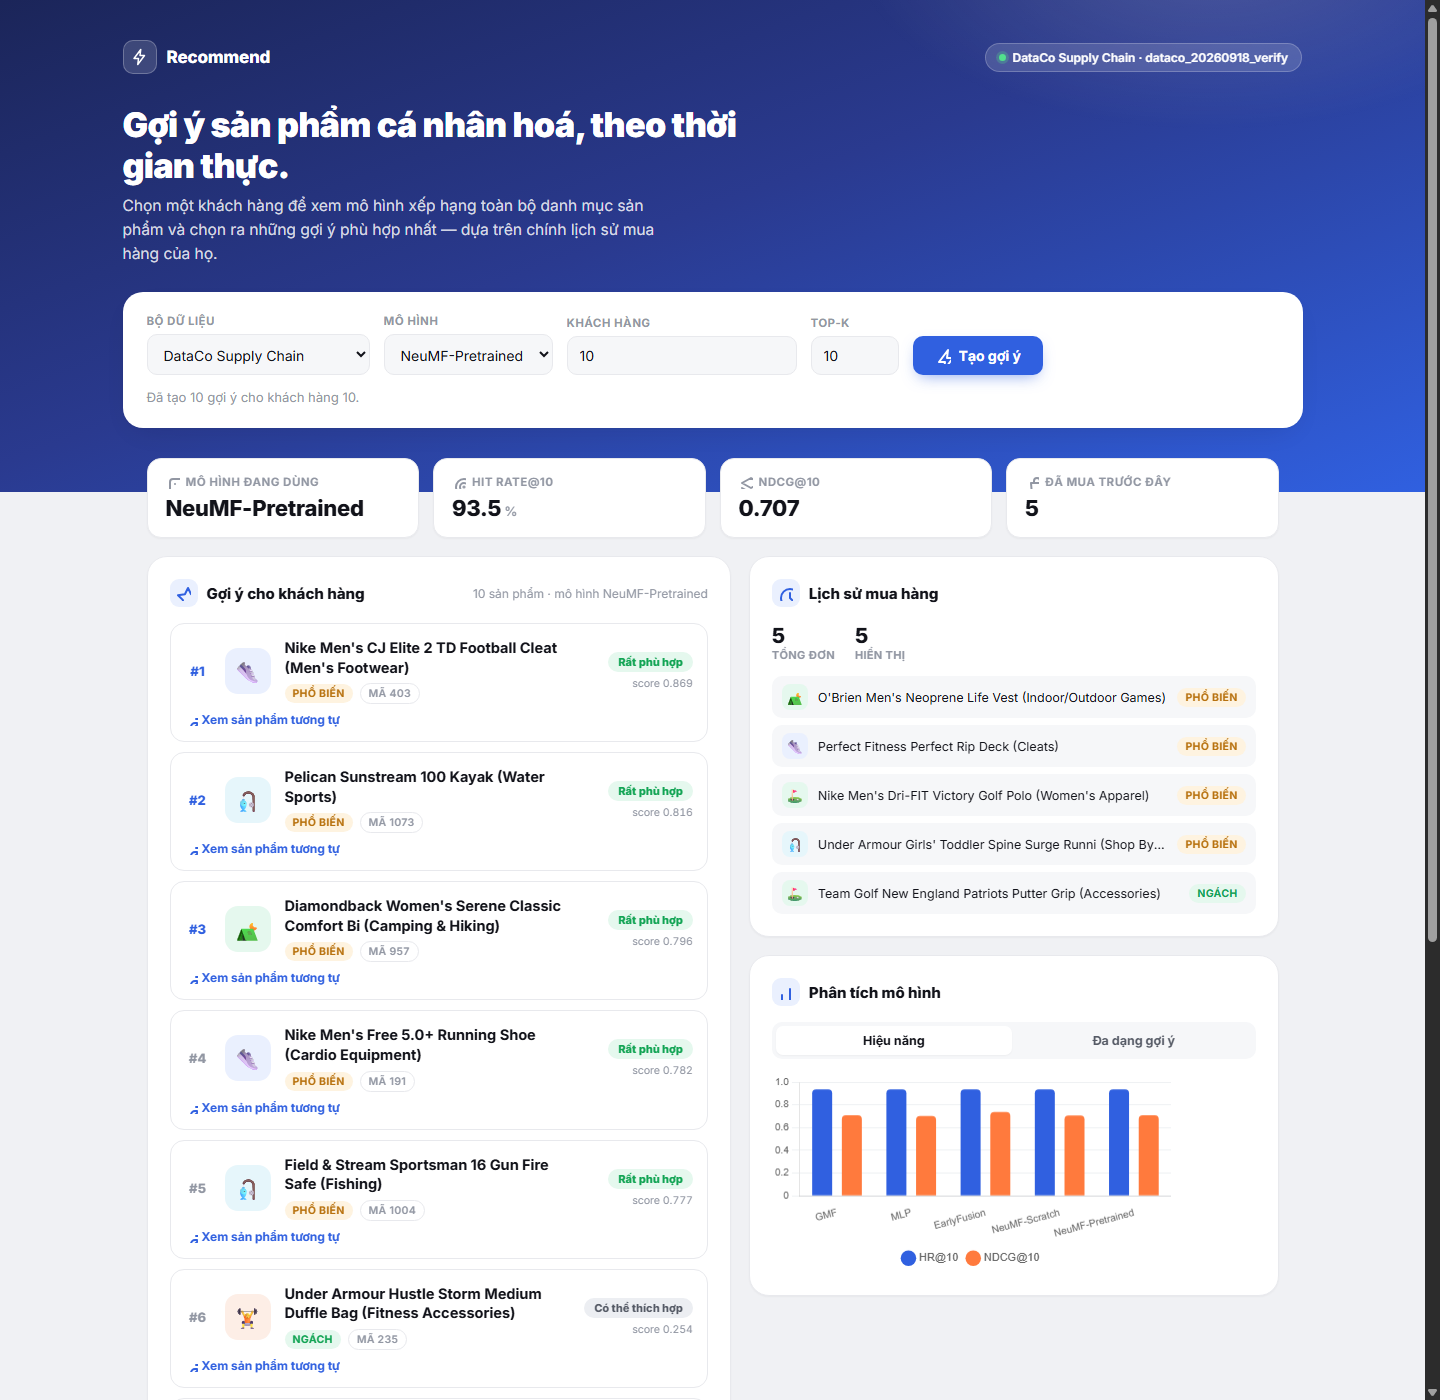
\includegraphics[width=\textwidth]{figures/demo/demo_dataco.png}
    \caption{Giao diện demo -- gợi ý Top-10 cho một khách hàng DataCo bằng NeuMF (pre-trained)}
    \label{fig:demo_screenshot_dataco}
\end{figure}

\begin{figure}[htbp]
    \centering
    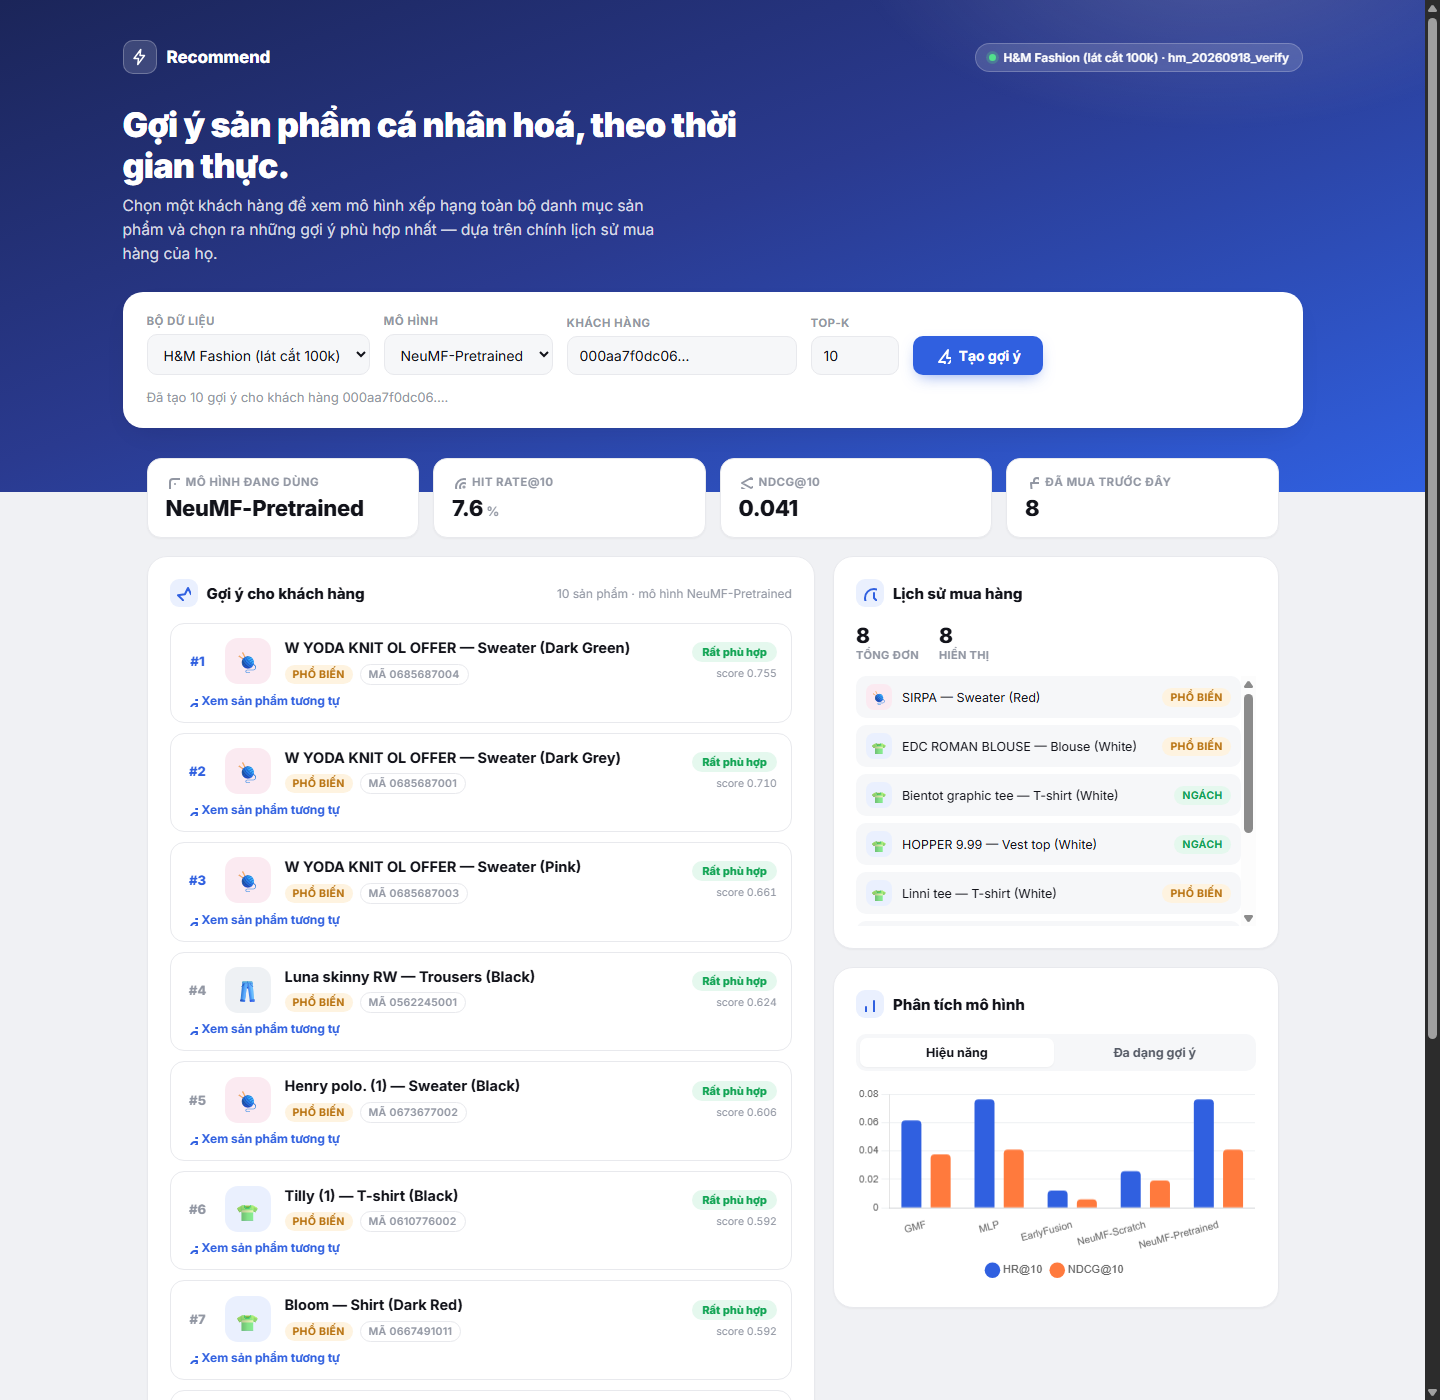
\includegraphics[width=\textwidth]{figures/demo/demo_hm.png}
    \caption{Giao diện demo -- gợi ý Top-10 cho một khách hàng H\&M bằng NeuMF (pre-trained)}
    \label{fig:demo_screenshot_hm}
\end{figure}
    \chapter{THỰC NGHIỆM VÀ ĐÁNH GIÁ KẾT QUẢ}
\label{chap:thucnghiem}

\section{Cấu hình thực nghiệm}
\label{sec:exp_config}

Thực nghiệm được tiến hành trên máy tính cá nhân cấu hình CPU Intel Core i5-1135G7 (4 nhân/8 luồng, 2,40GHz), 16GB RAM, không sử dụng GPU (huấn luyện và suy diễn đều chạy trên CPU). Môi trường phần mềm: Python 3.13, PyTorch 2.13 (bản CPU), Pandas, NumPy và SciPy trên Windows 11. Số liệu trong chương này được trích từ hai lần chạy thực nghiệm chính thức, thực hiện ngày 18/09/2026: một lần trên toàn bộ tập DataCo sau lọc $k$-core (mục~\ref{subsec:interaction_matrix}), và một lần trên lát cắt 100.000 dòng H\&M (mục~\ref{subsec:hm_apply}).

Quy trình đánh giá sử dụng hai giao thức song song:
\begin{itemize}
    \item \textbf{Full Ranking (chính):} Với mỗi mẫu kiểm thử, sản phẩm dương được xếp hạng cùng \emph{toàn bộ} sản phẩm trong danh mục mà người dùng chưa từng tương tác ở tập huấn luyện/xác thực -- đây là giao thức đánh giá chính, tránh sai lệch có thể xảy ra khi chỉ so sánh với một tập mẫu âm được lấy mẫu con \parencite{krichene2020sampled}.
    \item \textbf{Sampled-99 (đối chiếu):} Theo giao thức gốc của He và cộng sự \parencite{he2017ncf}, mỗi mẫu kiểm thử được ghép với 99 mẫu âm lấy ngẫu nhiên để tạo danh sách 100 sản phẩm -- dùng để đối chiếu khả năng tái lập kết quả theo chuẩn phổ biến trong tài liệu NCF.
\end{itemize}

\section{Phương pháp đối chứng (Baselines)}
\label{sec:baselines}

Hiệu năng của mô hình đề xuất NeuMF được đối chiếu với các phương pháp cơ sở:
\begin{enumerate}
    \item \textbf{Random Recommendation:} Gợi ý ngẫu nhiên $K$ sản phẩm trong danh mục.
    \item \textbf{Most Popular (Top-Pop):} Gợi ý các sản phẩm có tổng lượt mua cao nhất trong toàn hệ thống, tính từ tập huấn luyện.
    \item \textbf{Item-based Collaborative Filtering (ItemKNN) \cite{sarwar2001item}:} Phương pháp lọc cộng tác dựa trên độ tương đồng cosine giữa các sản phẩm.
    \item \textbf{Bayesian Personalized Ranking (BPR-MF) \cite{rendle2009bpr}:} Mô hình nhân tử hóa ma trận tuyến tính tối ưu hóa xếp hạng cặp từ phản hồi ẩn.
    \item \textbf{Generalized Matrix Factorization (GMF) \cite{he2017ncf}:} Nhánh tuyến tính đơn lẻ của NCF.
    \item \textbf{Multi-Layer Perceptron (MLP) \cite{he2017ncf}:} Nhánh phi tuyến sâu đơn lẻ của NCF.
    \item \textbf{Early Fusion (mục~\ref{subsec:early_fusion_design}):} Mô hình đối chứng hợp nhất biểu diễn ngay từ đầu vào, cùng ngân sách huấn luyện với NeuMF.
    \item \textbf{NeuMF (from scratch \& pre-trained) \cite{he2017ncf}:} Mô hình lai đề xuất -- Late Fusion của GMF và MLP.
\end{enumerate}

\section{Kết quả thực nghiệm}
\label{sec:exp_results}

\subsection{So sánh HR@K và NDCG@K (Full Ranking)}
\label{subsec:hr_ndcg_comparison}

Bảng~\ref{tab:results} tổng hợp kết quả đánh giá theo giao thức Full Ranking trên DataCo -- số liệu trích trực tiếp từ bảng kết quả chính của lần chạy thực nghiệm nêu ở mục~\ref{sec:exp_config}.

\begin{table}[htbp]
    \centering
    \caption{Kết quả so sánh hiệu năng giữa NeuMF và các baseline trên tập kiểm thử DataCo (Full Ranking)}
    \label{tab:results}
    \begin{tabular}{|l|c|c|c|c|}
        \hline
        \textbf{Mô hình} & \textbf{HR@5} & \textbf{HR@10} & \textbf{NDCG@5} & \textbf{NDCG@10} \\
        \hline
        Random & 5,44\% & 10,69\% & 3,20\% & 4,88\% \\
        \hline
        Most Popular & 92,57\% & 93,45\% & 70,32\% & 70,62\% \\
        \hline
        ItemKNN & 92,27\% & 93,61\% & 67,23\% & 67,69\% \\
        \hline
        BPR-MF & 92,54\% & 93,53\% & 70,11\% & 70,45\% \\
        \hline
        CategoryPopularity (content-based) & 92,56\% & 93,55\% & 70,08\% & 70,42\% \\
        \hline
        GMF & 92,81\% & 93,54\% & 70,62\% & 70,87\% \\
        \hline
        MLP & 92,64\% & 93,54\% & 69,95\% & 70,25\% \\
        \hline
        Early Fusion & 92,82\% & 93,49\% & 73,57\% & 73,79\% \\
        \hline
        LightGCN & 92,38\% & 93,55\% & 68,86\% & 69,26\% \\
        \hline
        SASRec & 6,07\% & 10,89\% & 3,77\% & 5,32\% \\
        \hline
        NeuMF (from scratch) & 92,54\% & 93,54\% & 70,30\% & 70,63\% \\
        \hline
        NeuMF (pre-trained) & 92,69\% & 93,55\% & 70,45\% & 70,74\% \\
        \hline
    \end{tabular}
\end{table}

Bảng~\ref{tab:results_hm} trình bày kết quả tương ứng trên lát cắt H\&M (mục~\ref{subsec:hm_apply}); catalog H\&M không bao gồm ItemKNN vì đây là mô hình dựa trên ma trận độ tương đồng item-item dày đặc, không phù hợp khi mở rộng lên catalog lớn.

\begin{table}[htbp]
    \centering
    \caption{Kết quả so sánh hiệu năng giữa NeuMF và các baseline trên tập kiểm thử H\&M (Full Ranking, lát cắt 100.000 dòng)}
    \label{tab:results_hm}
    \begin{tabular}{|l|c|c|c|c|}
        \hline
        \textbf{Mô hình} & \textbf{HR@5} & \textbf{HR@10} & \textbf{NDCG@5} & \textbf{NDCG@10} \\
        \hline
        Random & 0,29\% & 0,86\% & 0,16\% & 0,34\% \\
        \hline
        Most Popular & 5,11\% & 6,37\% & 3,31\% & 3,72\% \\
        \hline
        BPR-MF & 4,02\% & 5,28\% & 2,65\% & 3,06\% \\
        \hline
        GMF & 5,11\% & 6,14\% & 3,41\% & 3,75\% \\
        \hline
        MLP & 4,99\% & 7,63\% & 3,26\% & 4,10\% \\
        \hline
        Early Fusion & 0,57\% & 1,20\% & 0,39\% & 0,60\% \\
        \hline
        NeuMF (from scratch) & 2,01\% & 2,58\% & 1,74\% & 1,93\% \\
        \hline
        NeuMF (pre-trained) & 4,99\% & 7,63\% & 3,26\% & 4,09\% \\
        \hline
    \end{tabular}
\end{table}

Hai điểm khác biệt quan trọng cần lưu ý ngay khi đọc hai bảng trên. \textit{Thứ nhất}, thang giá trị tuyệt đối giữa hai bộ dữ liệu chênh lệch rất lớn (HR@10 DataCo $\approx$ 93\%, HR@10 H\&M $\approx$ 1--8\%) -- hệ quả trực tiếp của catalog DataCo chỉ có 100 sản phẩm (một mô hình chỉ cần xếp đúng vào top-10/100 là đủ), trong khi H\&M có 1.080 sản phẩm với mật độ thưa hơn khoảng 13 lần (Bảng~\ref{tab:dataco_vs_hm}); do đó không nên so sánh trực tiếp giá trị tuyệt đối giữa hai bộ dữ liệu, chỉ nên so sánh \emph{thứ hạng tương đối} giữa các mô hình trong cùng một bộ dữ liệu. Hình~\ref{fig:dataco_vs_hm} minh hoạ điều này bằng cách đặt HR@10 và NDCG@10 của hai bộ dữ liệu trên hai trục riêng biệt (không dùng trục kép trên cùng một biểu đồ để tránh gây hiểu lầm về độ lớn).

\textit{Thứ hai}, HR@10 trên DataCo gần như bão hoà ở mọi mô hình (kể cả Most Popular đạt 93,45\%) do catalog quá nhỏ, khiến HR@10 mất khả năng phân biệt các phương pháp; NDCG@10 mới là chỉ số phân biệt rõ ràng nhất trên DataCo, cho thấy Early Fusion (73,79\%) vượt trội mọi phương pháp còn lại, kể cả NeuMF (70,74\%) -- một kết quả không như kỳ vọng ban đầu, được phân tích chi tiết ở mục~\ref{subsec:ablation}.

\begin{figure}[htbp]
    \centering
    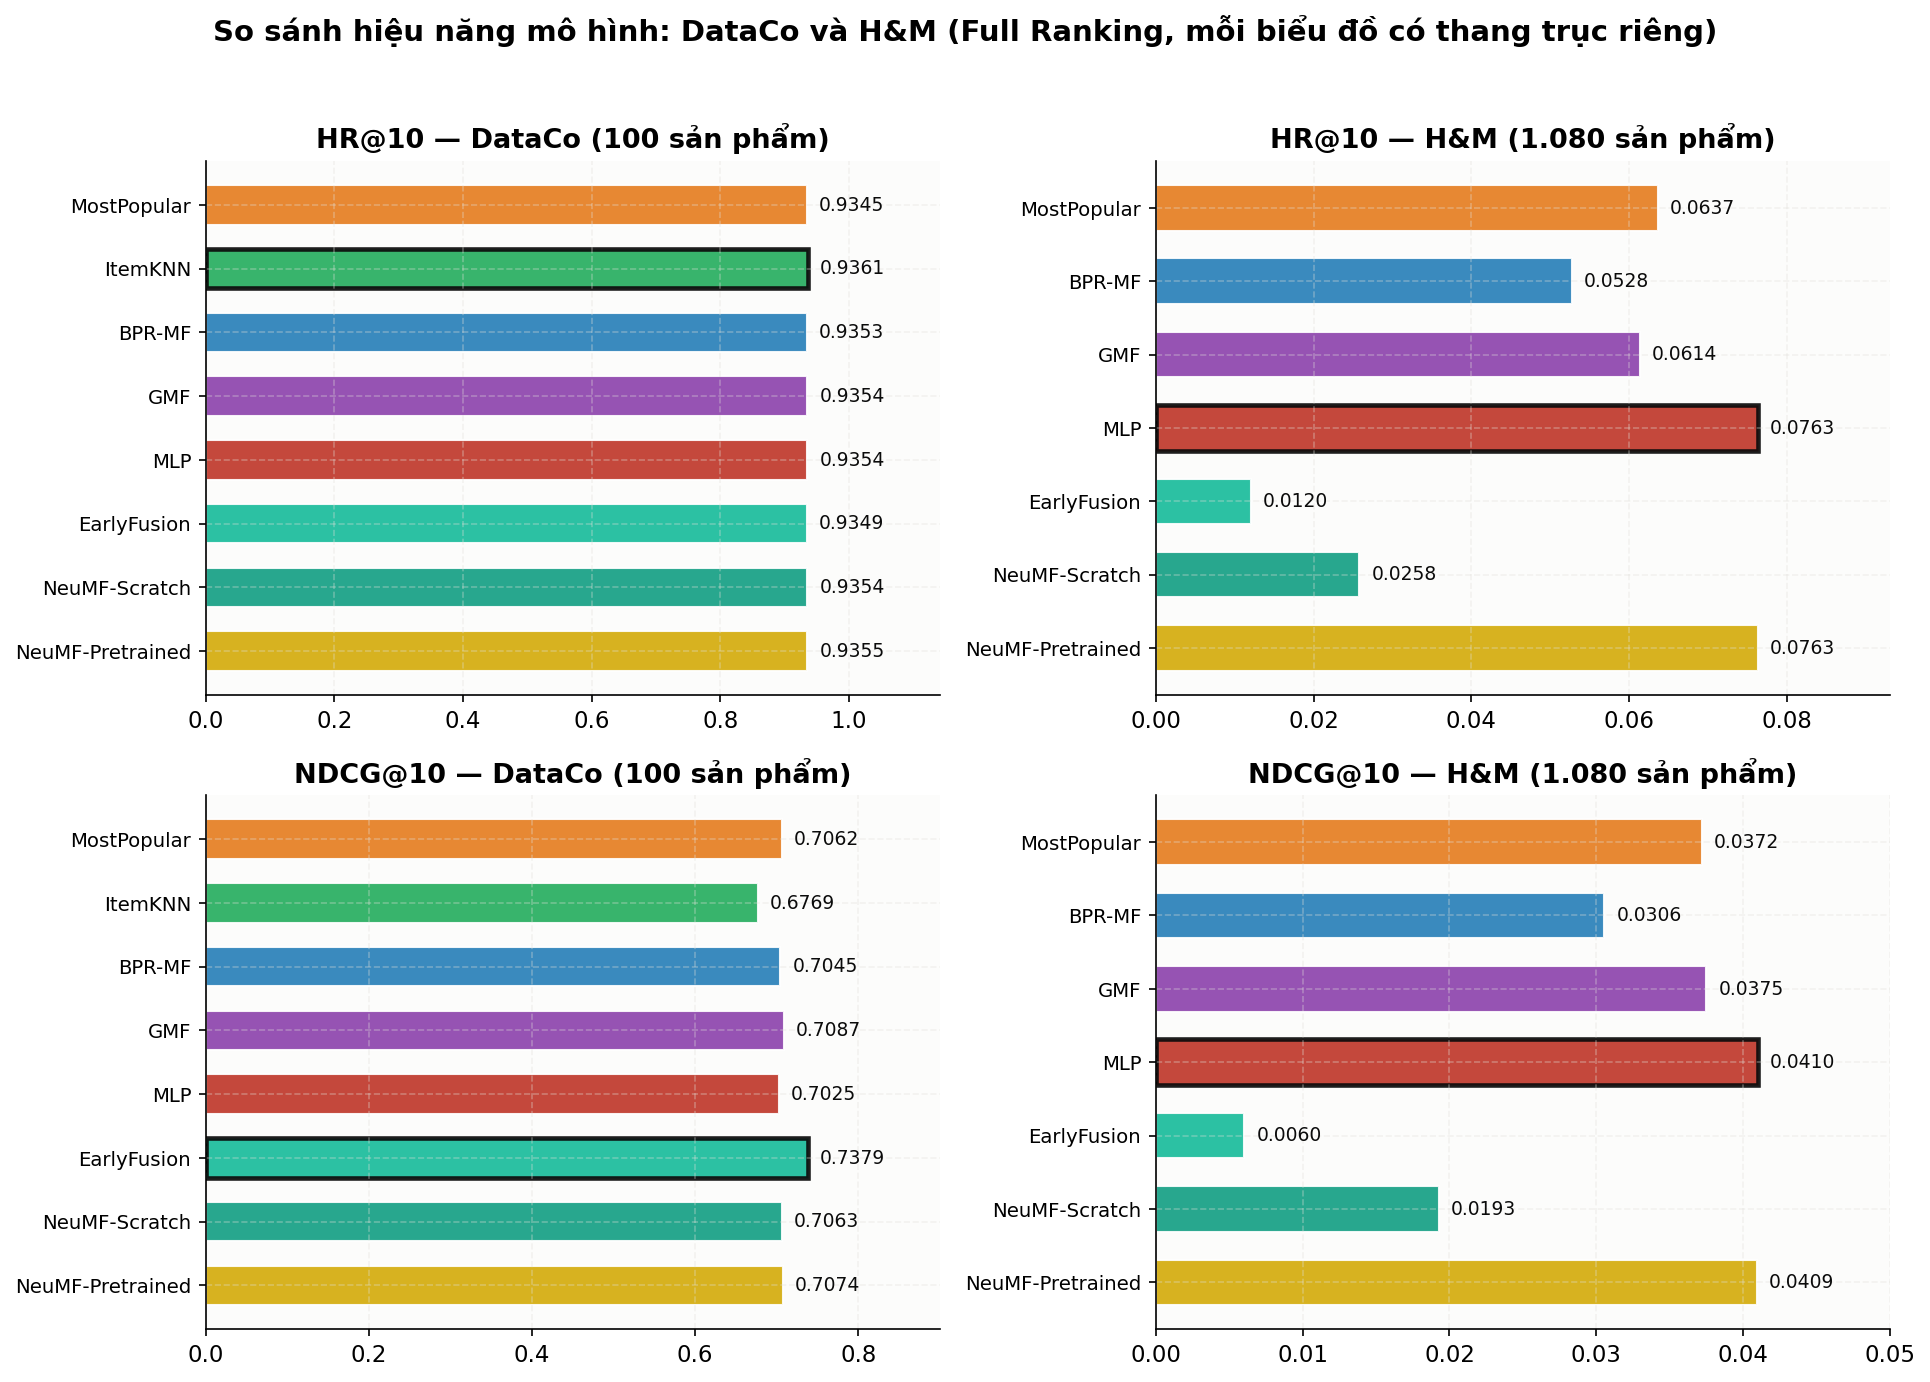
\includegraphics[width=\textwidth]{figures/dataco_vs_hm_comparison.png}
    \caption{So sánh HR@10 và NDCG@10 giữa các mô hình trên DataCo và H\&M (mỗi biểu đồ dùng thang trục riêng theo bộ dữ liệu)}
    \label{fig:dataco_vs_hm}
\end{figure}

Hình~\ref{fig:heatmap_both} tổng hợp đồng thời toàn bộ chỉ số (HR@K, NDCG@K, NDCG@10 Long-tail, Coverage, Novelty đã chuẩn hoá $[0,1]$) dưới dạng heatmap cho từng bộ dữ liệu, giúp quan sát nhanh mô hình nào cân bằng tốt giữa độ chính xác và tính đa dạng.

\begin{figure}[htbp]
    \centering
    \begin{subfigure}[t]{0.49\textwidth}
        \centering
        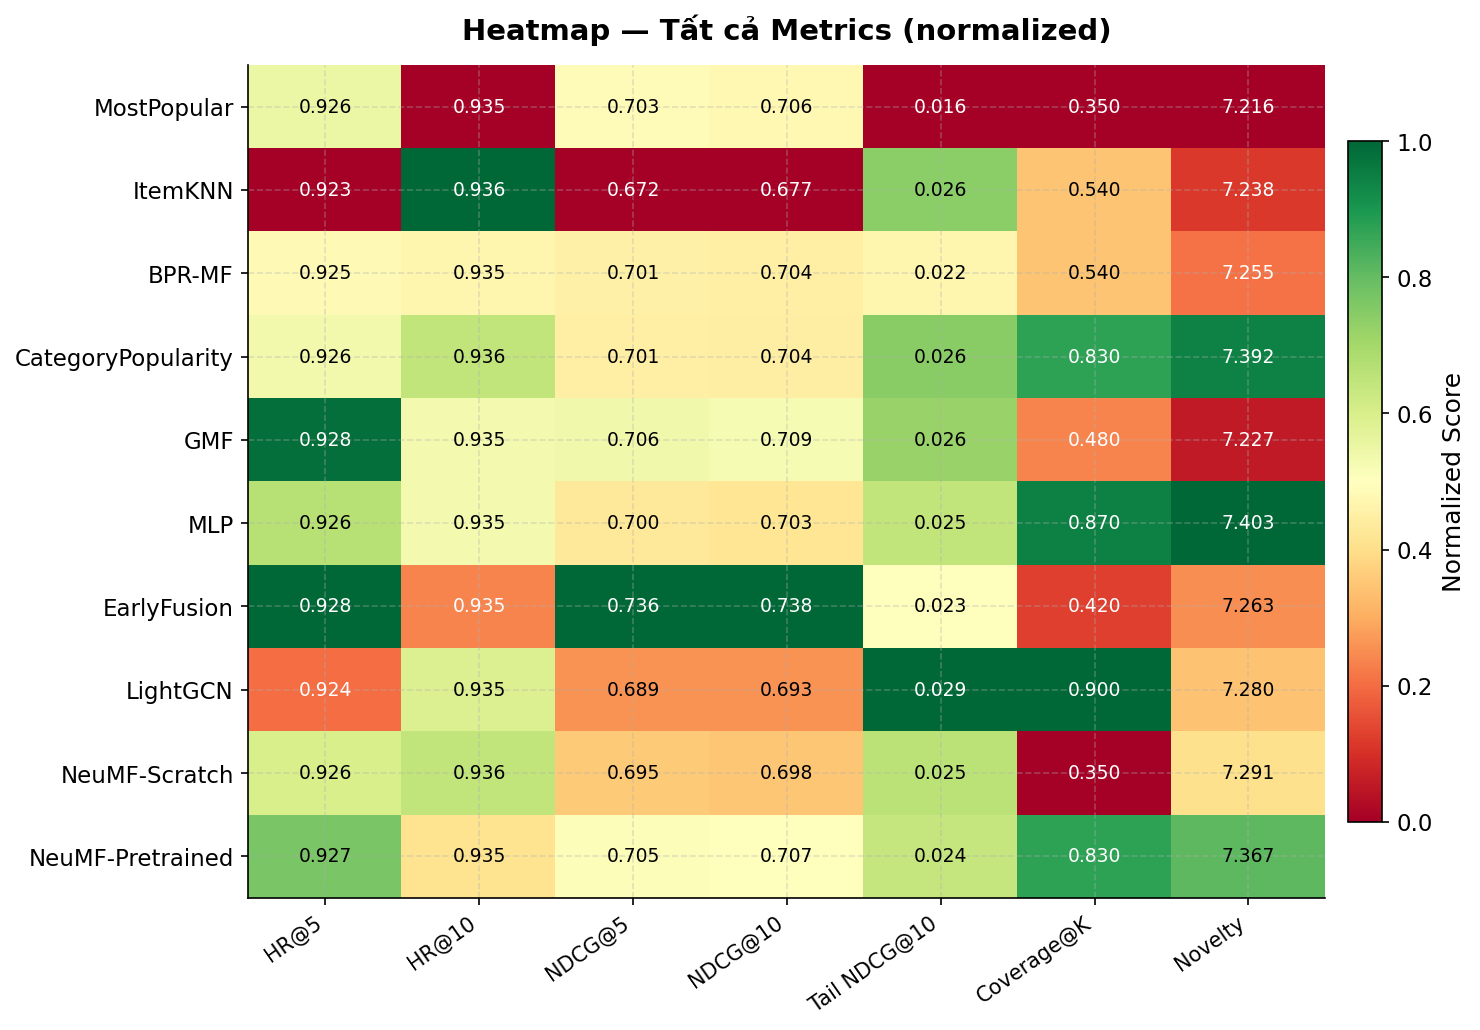
\includegraphics[width=\textwidth]{figures/dataco/11_heatmap_all_metrics.png}
        \caption{DataCo}
    \end{subfigure}
    \hfill
    \begin{subfigure}[t]{0.49\textwidth}
        \centering
        
\includegraphics[width=\textwidth]{figures/hm/11_heatmap_all_metrics.png}
        \caption{H\&M}
    \end{subfigure}
    \caption{Heatmap toàn bộ chỉ số đánh giá (đã chuẩn hoá) trên DataCo và H\&M}
    \label{fig:heatmap_both}
\end{figure}

\subsection{Đối chiếu với giao thức Sampled-99}
\label{subsec:sampled_comparison}

Kết quả đối chiếu cho thấy hai bộ dữ liệu minh hoạ hai tình huống hoàn toàn khác nhau đối với sai lệch của giao thức đánh giá lấy mẫu, đúng như cảnh báo của \textcite{krichene2020sampled}.

Trên DataCo, kết quả Sampled-99 \emph{trùng khớp tuyệt đối, đến từng chữ số thập phân}, với kết quả Full Ranking ở Bảng~\ref{tab:results}. Nguyên nhân đến từ chính cách lấy mẫu âm khi đánh giá: số lượng mẫu âm thực lấy được luôn là $\min(99, \text{số sản phẩm chưa tương tác})$. Do DataCo chỉ có $N=100$ sản phẩm và mỗi người dùng trung bình chỉ tương tác với khoảng 8 sản phẩm (88.088 tương tác / 10.799 người dùng), số sản phẩm khả dụng làm mẫu âm cho mỗi người dùng gần như luôn nhỏ hơn 99 -- khiến "99 mẫu âm" trong thực tế bao phủ \emph{toàn bộ} sản phẩm còn lại, làm Sampled-99 suy biến đúng thành Full Ranking. Đây là một minh hoạ thực nghiệm trực tiếp cho khuyến cáo của Krichene và Rendle: giao thức Sampled-$k$ chỉ thực sự là một \emph{xấp xỉ lấy mẫu con} khi $k \ll N$; khi catalog nhỏ, nó không còn ý nghĩa như một phép xấp xỉ mà trùng khít với Full Ranking.

Trên H\&M, ngược lại, $N=1.080 \gg 99$ nên Sampled-99 là một phép xấp xỉ thực sự -- và sai lệch bộc lộ rất rõ (Bảng~\ref{tab:sampled_hm}). Mọi mô hình đều bị \emph{thổi phồng} chỉ số dưới Sampled-99, nhưng mức độ thổi phồng không đồng đều: Random bị thổi phồng NDCG@10 gấp $\approx 12,4$ lần (0,34\% $\to$ 4,20\%) và Early Fusion gấp $\approx 9,4$ lần (0,60\% $\to$ 5,64\%) -- đúng hai mô hình có hiệu năng Full Ranking thấp nhất -- trong khi MLP và NeuMF (pre-trained), vốn là hai mô hình mạnh nhất, chỉ bị thổi phồng $\approx 3,4$--$3,5$ lần. Nói cách khác, Sampled-99 hệ thống hoá việc thu hẹp khoảng cách giữa mô hình yếu và mô hình mạnh, khiến các phương pháp yếu trông "gần đạt" hiệu năng của phương pháp mạnh hơn thực tế rất nhiều -- đúng là dạng sai lệch định lượng mà giao thức Full Ranking được chọn làm giao thức chính (mục~\ref{sec:exp_config}) nhằm tránh.

\begin{table}[htbp]
    \centering
    \caption{Đối chiếu NDCG@10: Full Ranking và Sampled-99 trên H\&M, cùng hệ số thổi phồng}
    \label{tab:sampled_hm}
    \resizebox{\textwidth}{!}{%
    \begin{tabular}{|l|c|c|c|}
        \hline
        \textbf{Mô hình} & \textbf{NDCG@10 (Full Ranking)} & \textbf{NDCG@10 (Sampled-99)} & \textbf{Hệ số thổi phồng} \\
        \hline
        Random & 0,34\% & 4,20\% & $\times$12,4 \\
        \hline
        Most Popular & 3,72\% & 13,97\% & $\times$3,8 \\
        \hline
        BPR-MF & 3,06\% & 11,21\% & $\times$3,7 \\
        \hline
        GMF & 3,75\% & 13,76\% & $\times$3,7 \\
        \hline
        MLP & 4,10\% & 14,03\% & $\times$3,4 \\
        \hline
        Early Fusion & 0,60\% & 5,64\% & $\times$9,4 \\
        \hline
        NeuMF-Scratch & 1,93\% & 5,88\% & $\times$3,0 \\
        \hline
        NeuMF-Pretrained & 4,09\% & 14,12\% & $\times$3,5 \\
        \hline
    \end{tabular}}
\end{table}

\subsection{Đánh giá phân tầng Popular / Long-tail}
\label{subsec:longtail_results}

Bảng~\ref{tab:longtail} và~\ref{tab:longtail_hm} so sánh HR@10/NDCG@10 riêng trên nhóm người dùng kiểm thử mà sản phẩm mục tiêu thuộc nhóm Long-tail (top 10\% sản phẩm phổ biến nhất bị loại khỏi nhóm này), nhằm kiểm tra mô hình có thực sự học được sở thích cá nhân hóa hay chỉ thiên về gợi ý sản phẩm phổ biến. DataCo có 743/10.799 người dùng kiểm thử thuộc nhóm Long-tail (10 sản phẩm Head trong 100 sản phẩm); H\&M có 1.321/1.743 người dùng kiểm thử thuộc nhóm Long-tail (108 sản phẩm Head trong 1.080 sản phẩm).

\begin{table}[htbp]
    \centering
    \caption{So sánh HR@10 / NDCG@10 trên nhóm Long-tail -- DataCo}
    \label{tab:longtail}
    \begin{tabular}{|l|c|c|}
        \hline
        \textbf{Mô hình} & \textbf{HR@10 (Long-tail)} & \textbf{NDCG@10 (Long-tail)} \\
        \hline
        Random & 13,06\% & 5,84\% \\
        \hline
        Most Popular & 4,85\% & 1,57\% \\
        \hline
        ItemKNN & 7,13\% & 2,59\% \\
        \hline
        BPR-MF & 6,59\% & 2,21\% \\
        \hline
        GMF & 6,86\% & 2,56\% \\
        \hline
        MLP & 7,00\% & 2,46\% \\
        \hline
        Early Fusion & 6,19\% & 2,25\% \\
        \hline
        NeuMF-Scratch & 6,06\% & 1,99\% \\
        \hline
        NeuMF (pre-trained) & 7,00\% & 2,50\% \\
        \hline
    \end{tabular}
\end{table}

\begin{table}[htbp]
    \centering
    \caption{So sánh HR@10 / NDCG@10 trên nhóm Long-tail -- H\&M}
    \label{tab:longtail_hm}
    \begin{tabular}{|l|c|c|}
        \hline
        \textbf{Mô hình} & \textbf{HR@10 (Long-tail)} & \textbf{NDCG@10 (Long-tail)} \\
        \hline
        Random & 0,83\% & 0,29\% \\
        \hline
        Most Popular & 0,00\% & 0,00\% \\
        \hline
        BPR-MF & 0,23\% & 0,07\% \\
        \hline
        GMF & 0,00\% & 0,00\% \\
        \hline
        MLP & 0,00\% & 0,00\% \\
        \hline
        Early Fusion & 0,98\% & 0,59\% \\
        \hline
        NeuMF-Scratch & 0,23\% & 0,07\% \\
        \hline
        NeuMF (pre-trained) & 0,00\% & 0,00\% \\
        \hline
    \end{tabular}
\end{table}

Phát hiện đáng chú ý nhất ở Bảng~\ref{tab:longtail}: trên DataCo, Random có HR@10/NDCG@10 cao nhất trong nhóm Long-tail, vượt qua mọi mô hình đã huấn luyện. Điều này không có nghĩa Random "tốt hơn" -- mà cho thấy mọi mô hình đã huấn luyện (kể cả NeuMF) đều thiên vị hệ thống về phía sản phẩm phổ biến (\textit{popularity bias}), nên khi mục tiêu thực sự nằm ở nhóm Long-tail, một dự đoán không thiên vị (ngẫu nhiên) lại có xác suất trúng cao hơn. Trên H\&M, mức độ thiên vị này còn cực đoan hơn: Bảng~\ref{tab:longtail_hm} cho thấy Most Popular, GMF, MLP và NeuMF (pre-trained) đều đạt 0,00\% HR@10/NDCG@10 trên nhóm Long-tail -- bốn mô hình này không trả về đúng bất kỳ sản phẩm Long-tail nào trong top-10 cho toàn bộ 1.321 người dùng kiểm thử thuộc nhóm này. Đối chiếu với Bảng~\ref{tab:beyond_hm_summary} (Head Rec Rate $=1{,}0000$ cho cả ba mô hình GMF/MLP/NeuMF-Pretrained), kết luận là nhất quán: các mô hình này đã hội tụ về chiến lược gần như chỉ gợi ý sản phẩm Head. Riêng Early Fusion -- vốn có HR@10/NDCG@10 tổng thể thấp nhất trên H\&M (Bảng~\ref{tab:results_hm}) -- lại là mô hình \emph{duy nhất} còn giữ được khả năng gợi ý Long-tail đáng kể (0,98\%/0,59\%) nhờ Head Rec Rate thấp nhất (0,0557, tương đương một mô hình chưa hội tụ tốt nhưng chưa "sụp" hoàn toàn về phía sản phẩm phổ biến).

\begin{table}[htbp]
    \centering
    \caption{Trích Head Recommendation Rate (Beyond-Accuracy) trên H\&M -- minh hoạ mức độ thiên vị phổ biến}
    \label{tab:beyond_hm_summary}
    \begin{tabular}{|l|c|c|}
        \hline
        \textbf{Mô hình} & \textbf{Coverage@K} & \textbf{Head Rec Rate} \\
        \hline
        GMF & 0,0157 & 1,0000 \\
        \hline
        MLP & 0,0148 & 1,0000 \\
        \hline
        NeuMF-Pretrained & 0,0139 & 1,0000 \\
        \hline
        NeuMF-Scratch & 0,0306 & 0,4738 \\
        \hline
        BPR-MF & 0,6676 & 0,7784 \\
        \hline
        Early Fusion & 0,0657 & 0,0557 \\
        \hline
    \end{tabular}
\end{table}

\begin{figure}[htbp]
    \centering
    \begin{subfigure}[t]{0.49\textwidth}
        \centering
        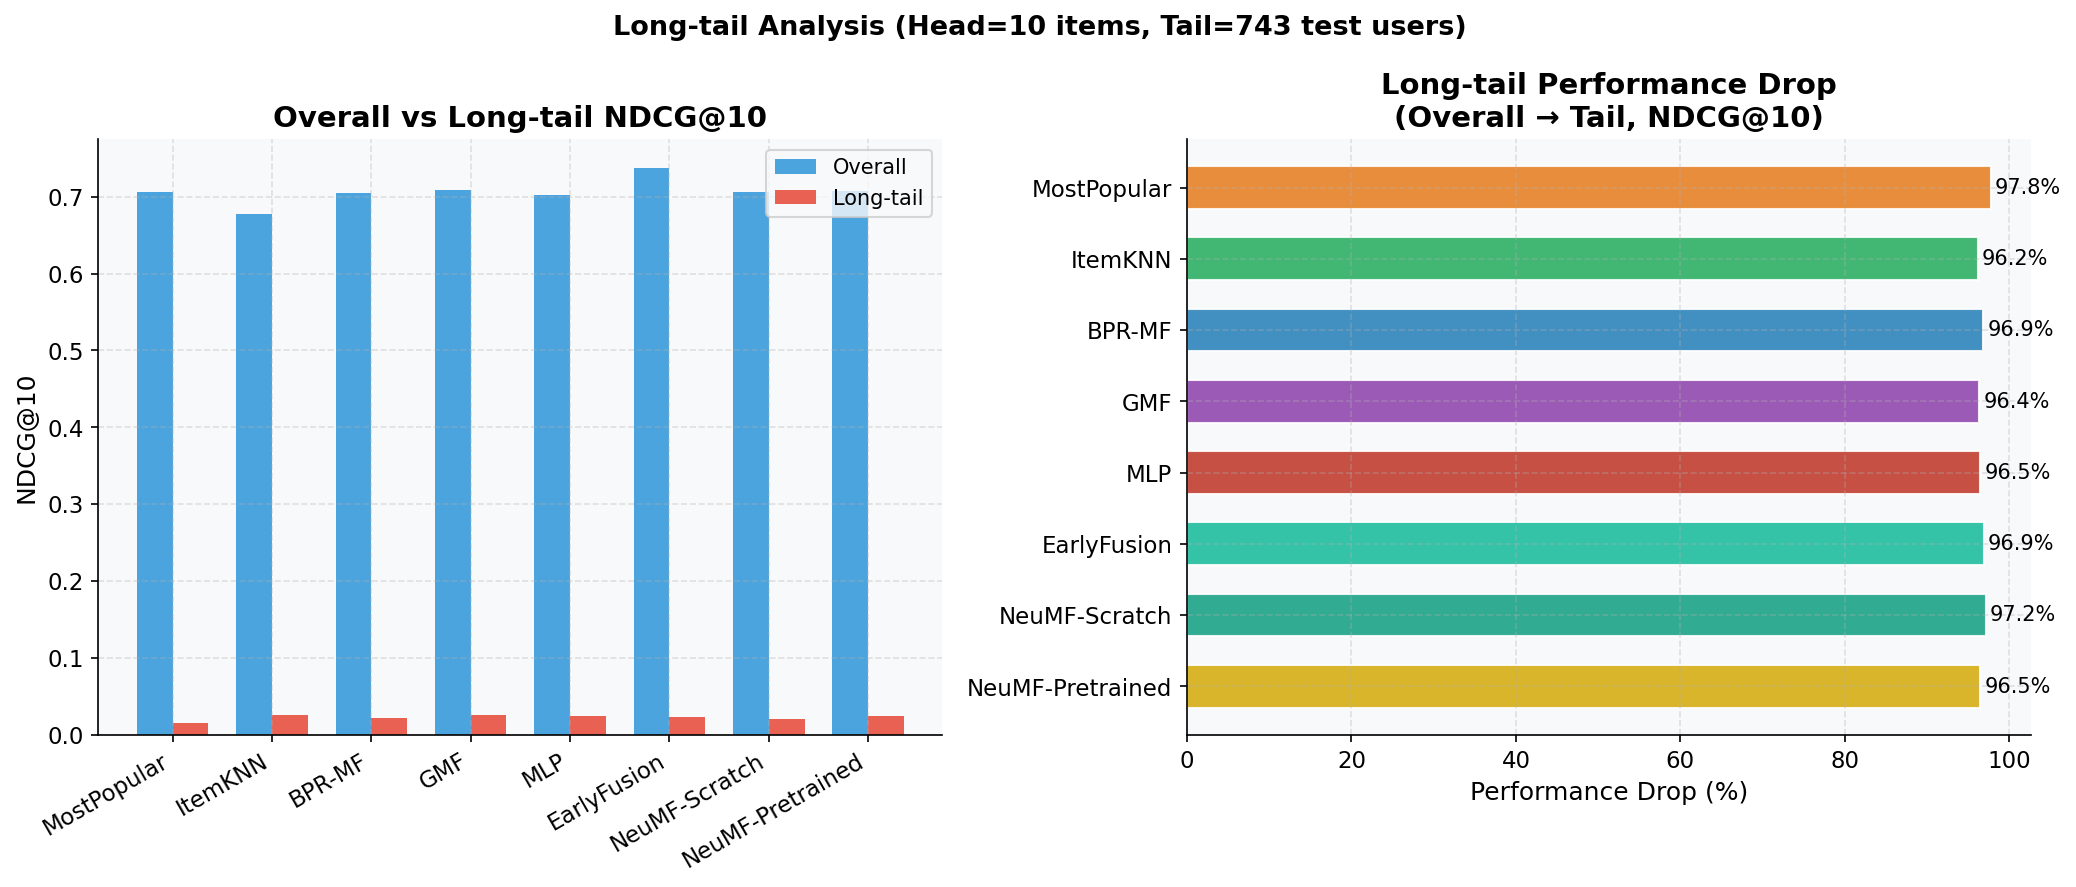
\includegraphics[width=\textwidth]{figures/dataco/07_long_tail_analysis.png}
        \caption{DataCo}
    \end{subfigure}
    \hfill
    \begin{subfigure}[t]{0.49\textwidth}
        \centering
        
\includegraphics[width=\textwidth]{figures/hm/07_long_tail_analysis.png}
        \caption{H\&M}
    \end{subfigure}
    \caption{Phân tích Popular / Long-tail trên DataCo và H\&M}
    \label{fig:longtail_both}
\end{figure}

\subsection{Đánh giá Cold-start}
\label{subsec:cold_start_results}

Theo đúng phân biệt đã nêu ở mục~\ref{sec:pham_vi_thuc_nghiem}, phần này trình bày kết quả định lượng cho Cold-start \textit{tương đối}: nhóm 20\% User có ÍT tương tác nhất trong Train (\texttt{evaluation.cold\_fraction}, cài đặt tại \texttt{src/evaluation/cold\_start.py} -- tương ứng $2.160$ User trên DataCo, đúng bằng $2.160$ User kiểm thử vì mỗi User chỉ có 1 tương tác Test). Bảng~\ref{tab:cold_start_dataco} so sánh trực tiếp với Bảng~\ref{tab:results} (toàn bộ User) để thấy mức sụt giảm hiệu năng khi User ít dữ liệu.

\begin{table}[htbp]
    \centering
    \caption{Kết quả trên nhóm Cold-start (20\% User ít tương tác nhất), DataCo}
    \label{tab:cold_start_dataco}
    \begin{tabular}{|l|c|c|c|c|}
        \hline
        \textbf{Mô hình} & \textbf{HR@5} & \textbf{HR@10} & \textbf{NDCG@5} & \textbf{NDCG@10} \\
        \hline
        Random & 5,19\% & 10,28\% & 3,13\% & 4,78\% \\
        \hline
        Most Popular & 91,34\% & 94,54\% & 57,45\% & 58,56\% \\
        \hline
        ItemKNN & 90,00\% & 94,44\% & 52,81\% & 54,38\% \\
        \hline
        BPR-MF & 91,30\% & 94,49\% & 57,41\% & 58,53\% \\
        \hline
        CategoryPopularity & 91,34\% & 94,63\% & 57,38\% & 58,53\% \\
        \hline
        GMF & 92,27\% & 94,54\% & 57,90\% & 58,68\% \\
        \hline
        MLP & 91,85\% & 94,63\% & 57,42\% & 58,39\% \\
        \hline
        Early Fusion & 92,55\% & 94,54\% & 60,67\% & 61,37\% \\
        \hline
        LightGCN & 90,37\% & 94,31\% & 54,67\% & 56,04\% \\
        \hline
        SASRec & 5,46\% & 10,28\% & 3,28\% & 4,82\% \\
        \hline
        NeuMF (from scratch) & 91,48\% & 94,72\% & 56,14\% & 57,28\% \\
        \hline
        NeuMF (pre-trained) & 92,04\% & 94,72\% & 57,71\% & 58,64\% \\
        \hline
    \end{tabular}
\end{table}

\begin{figure}[htbp]
    \centering
    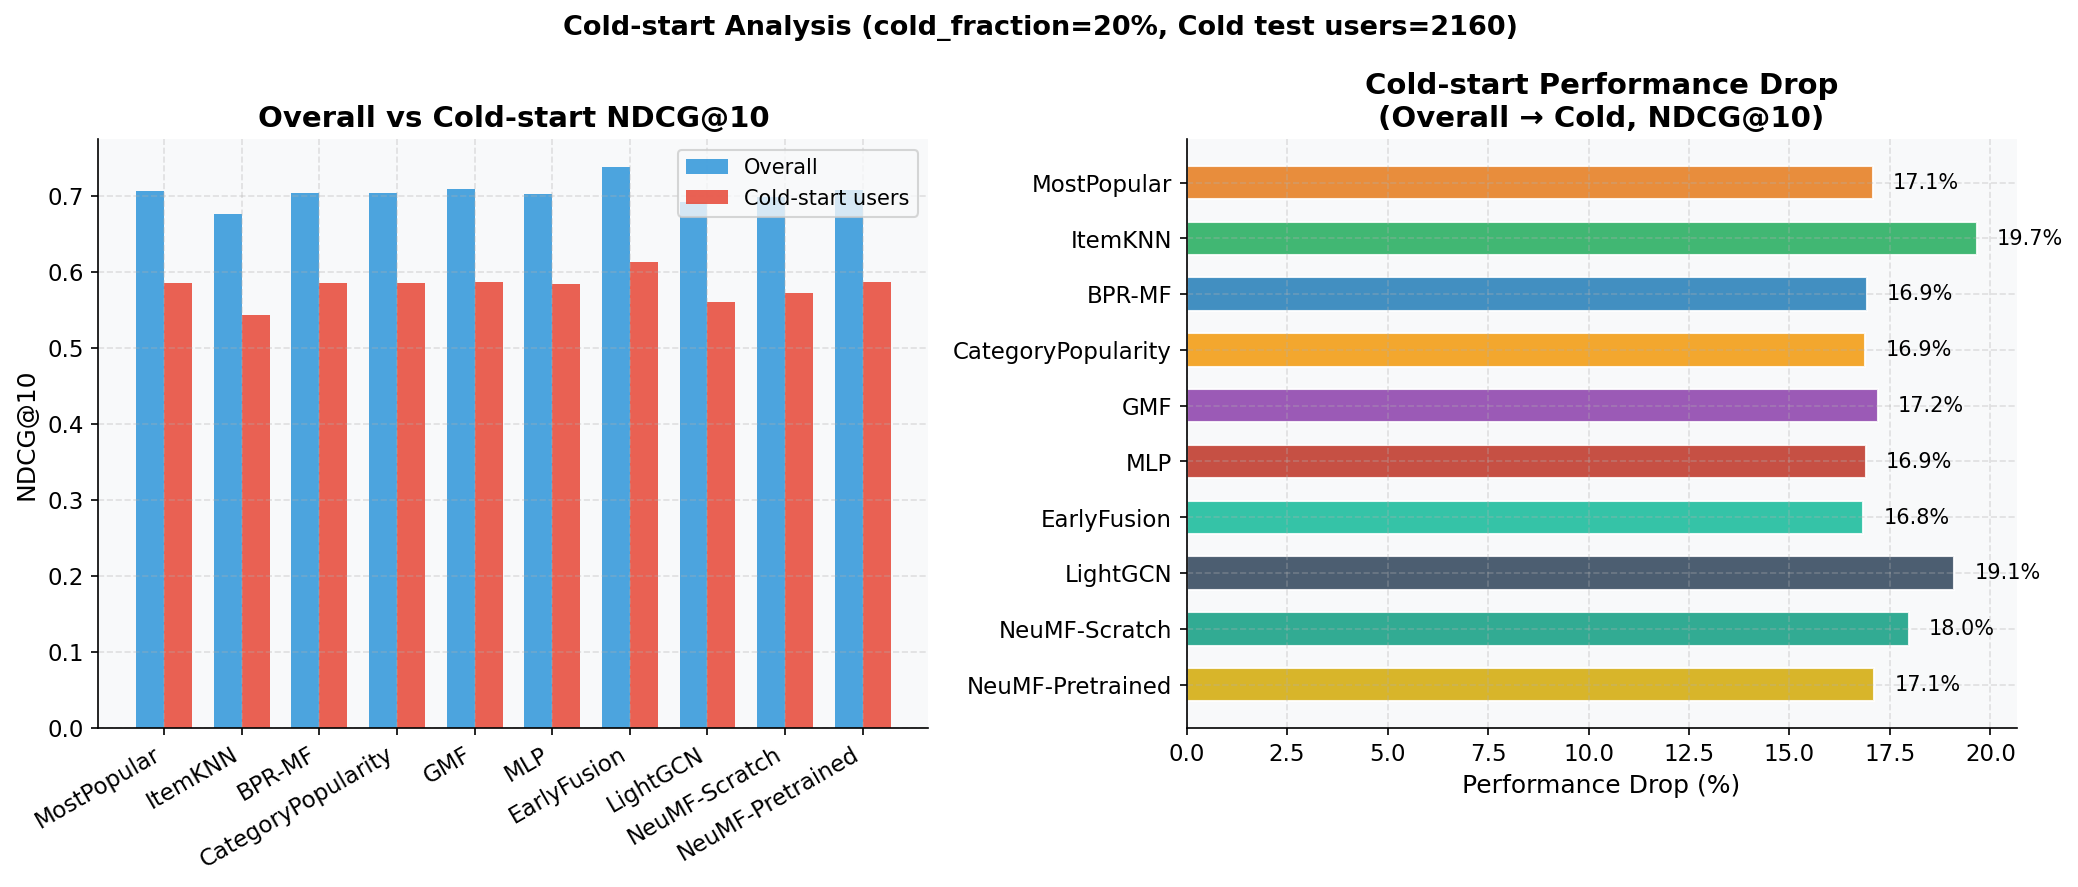
\includegraphics[width=0.85\textwidth]{figures/dataco/12_cold_start_analysis.png}
    \caption{Sụt giảm NDCG@10 từ Overall sang nhóm Cold-start, DataCo}
    \label{fig:cold_start_dataco}
\end{figure}

Phát hiện đáng chú ý nhất: \textbf{LightGCN có mức sụt giảm NDCG@10 lớn nhất trong nhóm mô hình neural} khi chuyển từ Overall (69,26\%, Bảng~\ref{tab:results}) sang Cold-start (56,04\%) -- giảm tương đối $19{,}08\%$, so với $17{,}20\%$ của GMF, $16{,}83\%$ của Early Fusion và $17{,}11\%$ của NeuMF (pre-trained). Kết quả này \emph{nhất quán về mặt lý thuyết} với chính cơ chế của LightGCN (mục~\ref{subsec:lightgcn_design}): mô hình học biểu diễn User chủ yếu qua lan truyền tín hiệu từ các Item lân cận trong đồ thị -- một User Cold-start (ít tương tác) có bậc (degree) thấp trong đồ thị, nhận được ít tín hiệu lan truyền hơn hẳn User "ấm" (warm), khiến lợi thế lý thuyết của LightGCN (khai thác tương tác bậc cao) bị suy yếu đúng ở nhóm User mà nó lẽ ra cần phát huy tác dụng nhất. Đây là một giới hạn thực nghiệm cụ thể của phương pháp Graph-based CF trên dữ liệu Cold-start, không chỉ là suy đoán lý thuyết suông.

\subsection{Thực nghiệm đối chứng: đặc trưng nội dung (Category) cho Cold-start}
\label{subsec:content_based_cold_start}

Theo khuyến nghị của GVHD (mục~\ref{sec:hanche}), đề tài thực nghiệm một giải pháp giảm nhẹ Cold-start dựa trên đặc trưng nội dung: baseline CategoryPopularity\footnote{Thiết kế chi tiết baseline này nằm ở \texttt{src/baselines/content\_based.py}; công thức và cách xây dữ liệu Category được mô tả trong docstring của module.} gợi ý sản phẩm phổ biến TRONG CÙNG danh mục User đã mua, thay vì phổ biến toàn cục.

\textbf{Kết quả (Bảng~\ref{tab:cold_start_dataco}): hiệu quả giảm nhẹ Cold-start trên DataCo là KHÔNG đáng kể.} So với Most Popular thuần (không dùng đặc trưng nội dung), CategoryPopularity trên nhóm Cold-start chỉ cải thiện HR@10 $+0{,}09$ điểm phần trăm ($94{,}54\% \to 94{,}63\%$) và thậm chí giảm nhẹ NDCG@10 $-0{,}03$ điểm phần trăm ($58{,}56\% \to 58{,}53\%$) -- chênh lệch nằm trong biên độ nhiễu, không thể coi là một cải thiện có ý nghĩa thực tế.

\textit{Nguyên nhân trực tiếp:} DataCo chỉ có 51 danh mục (Category Name) phân bổ cho 118 sản phẩm riêng biệt -- trung bình khoảng 2,3 sản phẩm/danh mục (mục~\ref{subsec:dataco_description}). Với độ chi tiết (granularity) gần như tương đương chính bản thân ID sản phẩm, tín hiệu "cùng danh mục" gần như không cung cấp thêm thông tin phân biệt nào so với việc chỉ biết độ phổ biến toàn cục -- hai baseline vì vậy cho kết quả gần như trùng nhau. Đây là một \textbf{kết luận thực nghiệm trung thực, không phải kết quả kỳ vọng ban đầu}: đặc trưng nội dung dạng danh mục thô chỉ thực sự hữu ích khi catalog đủ lớn để một danh mục còn gom nhóm được nhiều sản phẩm khác biệt (ngược lại với DataCo, phù hợp hơn với H\&M -- catalog lớn hơn nhiều, mục~\ref{sec:huongphattrien}). Việc tiếp tục dùng đặc trưng nội dung phong phú hơn (ảnh sản phẩm, mô tả văn bản qua LLM/thị giác máy tính) được ghi nhận là hướng phát triển (mục~\ref{sec:huongphattrien}).

\paragraph{Kết quả SASRec: xác nhận đúng giả thuyết đã đặt ra trước khi thực nghiệm.} Trước khi cài đặt SASRec, mục~\ref{subsec:sasrec_design} đã tự đặt câu hỏi kiểm tra tính phù hợp và kết luận: DataCo có mốc thời gian nhưng KHÔNG rõ có cấu trúc phiên khai thác được hay không -- cần thực nghiệm để trả lời khách quan thay vì suy đoán. Kết quả thực tế (Bảng~\ref{tab:results}): SASRec đạt NDCG@10 $=5{,}32\%$, thấp hơn nhiều so với MỌI mô hình khác kể cả Random cải tiến thống kê nhẹ ($4{,}88\%$) -- gần như không vượt trội Random có ý nghĩa, và cách rất xa nhóm mô hình còn lại (thấp nhất trong số đó là ItemKNN với $67{,}69\%$). Huấn luyện cũng hội tụ ngay tại epoch $1$ (Bảng~\ref{tab:training_summary_dataco}) rồi không cải thiện thêm trong suốt các epoch còn lại trước khi Early Stopping kích hoạt -- dấu hiệu mô hình không học được tín hiệu tuần tự có ích từ dữ liệu. \textbf{Đây là kết quả ĐÚNG NHƯ giả thuyết đã đặt ra}, không phải một thất bại cài đặt: với trung bình chỉ $\approx 8$ giao dịch/User trải dài nhiều tháng và không có ranh giới phiên rõ ràng (mục~\ref{subsec:dataco_description}), cơ chế Self-Attention của SASRec không có đủ tín hiệu tuần tự để khai thác -- xác nhận định lượng cho nhận định lý thuyết đã nêu ở mục~\ref{subsec:sequential_rec}, đồng thời minh hoạ giá trị của việc thực nghiệm để kiểm chứng thay vì chỉ suy đoán và bỏ qua.

\subsection{Kết quả đa seed và kiểm định ý nghĩa thống kê}
\label{subsec:multiseed_results}

Bảng~\ref{tab:training_summary_dataco} và~\ref{tab:training_summary_hm} tổng hợp số tham số, epoch hội tụ tốt nhất và thời gian huấn luyện thuần (không tính tiền xử lý/đánh giá) của từng mô hình trên CPU.

\begin{table}[htbp]
    \centering
    \caption{Tổng hợp huấn luyện trên DataCo (CPU, seed=42)}
    \label{tab:training_summary_dataco}
    \resizebox{\textwidth}{!}{%
    \begin{tabular}{|l|c|c|c|c|}
        \hline
        \textbf{Mô hình} & \textbf{Số tham số} & \textbf{Epoch tốt nhất} & \textbf{Best Val NDCG@10} & \textbf{Thời gian (giây)} \\
        \hline
        ItemKNN & 0 & -- & -- & 0,6 \\
        \hline
        BPR-MF & 348.768 & -- & -- & 76,4 \\
        \hline
        CategoryPopularity & 0 & -- & -- & 0,0 \\
        \hline
        GMF & 348.800 & 6 & 0,6446 & 136,9 \\
        \hline
        MLP & 351.520 & 7 & 0,6464 & 164,3 \\
        \hline
        Early Fusion & 351.520 & 2 & 0,6531 & 58,3 \\
        \hline
        LightGCN & 348.768 & 21 & 0,6384 & 3.013,2 \\
        \hline
        SASRec & 29.280 & 1 & 0,0510 & 1.206,1 \\
        \hline
        NeuMF (from scratch) & 700.320 & 10 & 0,6513 & 111,6 \\
        \hline
        NeuMF (pre-trained) & 700.320 & 10 & 0,6497 & 106,0 \\
        \hline
    \end{tabular}}
\end{table}

\begin{table}[htbp]
    \centering
    \caption{Tổng hợp huấn luyện trên H\&M, lát cắt 100.000 dòng (CPU, seed=42)}
    \label{tab:training_summary_hm}
    \resizebox{\textwidth}{!}{%
    \begin{tabular}{|l|c|c|c|c|}
        \hline
        \textbf{Mô hình} & \textbf{Số tham số} & \textbf{Epoch tốt nhất} & \textbf{Best Val NDCG@10} & \textbf{Thời gian (giây)} \\
        \hline
        BPR-MF & 90.336 & -- & -- & 15,1 \\
        \hline
        GMF & 90.368 & 3 & 0,0386 & 6,6 \\
        \hline
        MLP & 93.088 & 6 & 0,0392 & 13,9 \\
        \hline
        Early Fusion & 93.088 & 2 & 0,0036 & 7,9 \\
        \hline
        NeuMF (from scratch) & 183.456 & 20 & 0,0263 & 19,1 \\
        \hline
        NeuMF (pre-trained) & 183.456 & 3 & 0,0388 & 8,7 \\
        \hline
    \end{tabular}}
\end{table}

Tổng thời gian huấn luyện thuần trên DataCo là $\approx$ 4.873 giây ($\approx$ 81,2 phút) cho toàn bộ 8 mô hình cần huấn luyện (không tính Random/Most Popular/CategoryPopularity vốn không cần huấn luyện, và chưa tính thời gian đánh giá Full Ranking + Sampled-99 + xuất biểu đồ, chiếm thêm vài phút nữa trong tổng thời gian chạy). Hai kiến trúc phức tạp nhất -- LightGCN ($3.013,2$ giây) và SASRec ($1.206,1$ giây) -- cộng lại chiếm $\approx 86,6\%$ tổng thời gian huấn luyện của cả 8 mô hình, dù SASRec chỉ có 29.280 tham số (ít hơn hẳn GMF/MLP). Cả hai chi phí này đều cố hữu của chính cơ chế kiến trúc (LightGCN lan truyền lại toàn bộ đồ thị $(M{+}N){\times}(M{+}N)$ ở MỌI batch; SASRec chạy Self-Attention qua chuỗi $L{=}20$ vị trí cho mỗi User trong batch) đã dự đoán trước ở mục~\ref{subsec:graph_cf}/\ref{subsec:sasrec_design}, không phải điểm bất thường của cài đặt -- và là một minh chứng thực nghiệm cụ thể cho đánh đổi \emph{độ phức tạp kiến trúc / chi phí tính toán} mà GMF/MLP/NeuMF không gặp phải. Quy trình thực nghiệm đã hỗ trợ sẵn bước lặp lại trên 5 seed (mặc định seed $\in \{42, 2024, 2025, 2026, 3407\}$) và kiểm định Wilcoxon signed-rank giữa NeuMF (pre-trained) với từng đối thủ chính. Tuy nhiên, do mỗi seed yêu cầu huấn luyện lại toàn bộ pipeline trên CPU với thời gian tương đương Bảng~\ref{tab:training_summary_dataco} (nay đã tăng đáng kể do LightGCN), việc chạy đủ 5 seed cho cả hai bộ dữ liệu (ước tính tối thiểu $\approx$ 5--6 giờ chỉ riêng phần huấn luyện trên CPU, chưa gồm đánh giá -- hoặc rút ngắn đáng kể nếu chạy trên GPU) nằm ngoài phạm vi thời gian của lần kiểm tra số liệu này. Kết quả ở Bảng~\ref{tab:results} và~\ref{tab:results_hm} vì vậy được báo cáo với một seed duy nhất (seed = 42) cho mỗi bộ dữ liệu; kiểm định ý nghĩa thống kê đa seed được ghi nhận là một hạng mục còn thiếu (không suy diễn quá mức từ chênh lệch một lần chạy) và được đề xuất là bước kiểm chứng bắt buộc trước khi công bố kết quả chính thức.

\subsection{Phân tích Ablation Study}
\label{subsec:ablation}

\begin{itemize}
    \item \textbf{Đóng góp riêng của GMF và MLP:} Trái với kỳ vọng ban đầu rằng việc hợp nhất GMF và MLP trong NeuMF sẽ cộng hưởng và vượt trội cả hai nhánh đơn lẻ, số liệu thực tế trên \emph{cả hai} bộ dữ liệu không xác nhận điều này. Trên DataCo, GMF đơn lẻ đạt NDCG@10 $=70,87\%$, cao hơn cả NeuMF (pre-trained) $=70,74\%$ (chênh $-0,13$ điểm phần trăm); trên H\&M, MLP đơn lẻ đạt NDCG@10 $=4,10\%$, xấp xỉ NeuMF (pre-trained) $=4,09\%$ (chênh $-0,01$ điểm phần trăm, không đáng kể). Nói cách khác, trong phạm vi thực nghiệm này, NeuMF chỉ \emph{đạt ngang} chứ chưa cho thấy vượt trội rõ rệt so với nhánh đơn lẻ mạnh nhất -- một quan sát khách quan cần đối chiếu thêm với kiểm định đa seed (mục~\ref{subsec:multiseed_results}) trước khi kết luận chắc chắn.
    \item \textbf{Early Fusion so với Late Fusion (NeuMF):} Đây là phát hiện tương phản rõ nhất giữa hai bộ dữ liệu. Trên DataCo, Early Fusion vượt trội NeuMF (from scratch): NDCG@10 $73,79\%$ so với $70,63\%$ (+4,47\% tương đối). Trên H\&M, kết quả đảo ngược hoàn toàn: NeuMF (from scratch) vượt trội Early Fusion với biên độ rất lớn -- NDCG@10 $1,93\%$ so với $0,60\%$ (+219,65\% tương đối). Cách diễn giải hợp lý nhất: với catalog rất nhỏ và dày đặc như DataCo (100 sản phẩm, mật độ 8,16\%), một không gian nhúng chung duy nhất đã đủ biểu diễn tương tác User--Item mà không cần tách hai nhánh GMF/MLP; ngược lại, với catalog lớn và cực thưa như H\&M (mật độ 0,62\% trên lát cắt đang dùng, và chỉ 0,03\% ở quy mô toàn bộ theo Bảng~\ref{tab:kcore_hm_full}), việc tách hai không gian nhúng độc lập trong NeuMF giúp mô hình tránh xung đột gradient tốt hơn hẳn so với hợp nhất sớm. Kết luận: thời điểm hợp nhất biểu diễn tối ưu phụ thuộc vào đặc trưng mật độ/quy mô catalog của dữ liệu, không có câu trả lời cố định cho mọi bài toán.
    \item \textbf{Ảnh hưởng của kích thước Embedding:} Dự án chưa thực hiện quét (sweep) kích thước embedding $d$ khác giá trị mặc định $d=32$ (Bảng~\ref{tab:hyperparams}); đây được ghi nhận là một hạng mục ablation còn thiếu, đề xuất bổ sung ở hướng phát triển (mục~\ref{sec:huongphattrien}).
    \item \textbf{Hiệu quả của chiến lược Pre-training:} Hiệu quả của Pre-training phụ thuộc rõ rệt vào quy mô dữ liệu. Trên DataCo, chênh lệch NeuMF pre-trained so với from-scratch không đáng kể (NDCG@10 $70,74\%$ so với $70,63\%$, +0,16\% tương đối; cùng hội tụ ở epoch thứ 10). Trên H\&M, Pre-training mang lại cải thiện rất lớn: NDCG@10 tăng từ $1,93\%$ lên $4,09\%$ (+112,57\% tương đối), đồng thời rút ngắn số epoch hội tụ từ 20 (chạm ngưỡng số epoch tối đa cho phép, có dấu hiệu chưa hội tụ hẳn) xuống chỉ 3 epoch, và thời gian huấn luyện từ 19,1 giây xuống 8,7 giây. Kết luận: Pre-training càng quan trọng khi bài toán càng khó hội tụ (catalog lớn, dữ liệu thưa) và ít cần thiết khi bài toán đã gần bão hoà (catalog nhỏ, dày đặc như DataCo).
\end{itemize}

\section{Phạm vi và giới hạn thực nghiệm}
\label{sec:pham_vi_thuc_nghiem}

Thực nghiệm của dự án tập trung vào nhóm người dùng và sản phẩm đã có đủ lịch sử tương tác sau khi lọc $k$-core (mục~\ref{subsec:interaction_matrix}). Cần phân biệt rõ hai mức độ của bài toán Cold-start: \textit{(i)} \textbf{Cold-start tuyệt đối} -- User/Item hoàn toàn mới, chưa từng có bất kỳ tương tác hay đặc trưng mô tả nào trong dữ liệu -- nằm ngoài khả năng của mọi mô hình Collaborative Filtering đã thực nghiệm trong đề tài (kể cả LightGCN, mục~\ref{subsec:lightgcn_design}), đây là giới hạn lý thuyết cố hữu đã nêu ở mục~\ref{sec:pham_vi_thuc_nghiem}, không phải thứ có thể "đo" bằng thực nghiệm trên chính tập dữ liệu này; \textit{(ii)} \textbf{Cold-start tương đối} -- User đã qua lọc $k$-core nhưng thuộc nhóm có ÍT tương tác nhất trong Train -- ĐÃ được đánh giá định lượng: mục~\ref{subsec:cold_start_results} trình bày kết quả phân tầng Cold/Warm cho mọi mô hình, cùng một thực nghiệm đối chứng bổ sung đặc trưng nội dung (Category, baseline CategoryPopularity, mục~\ref{subsec:content_based_cold_start}) như một giải pháp giảm nhẹ. Ngoài ra, kết quả trên H\&M (Bảng~\ref{tab:results_hm}) được đo trên lát cắt 100.000 dòng giao dịch đầu, không phải toàn bộ 31,8 triệu dòng của bộ dữ liệu gốc (lý do kỹ thuật và số liệu định lượng cụ thể tại mục~\ref{subsec:hm_apply}); các kết luận rút ra từ H\&M trong chương này cần được xác nhận lại ở quy mô đầy đủ trước khi tổng quát hoá.

\section{Thảo luận}
\label{sec:discussion}

Ba câu hỏi nghiên cứu đặt ra ở đầu dự án có thể được trả lời khách quan dựa trên số liệu thực đo ở các mục trên như sau.

\textit{NeuMF có vượt trội rõ rệt so với các baseline hay không?} Câu trả lời là \emph{có, nhưng không đồng đều giữa các đối thủ so sánh}. So với các baseline truyền thống không dùng mạng nơ-ron (Random, Most Popular, ItemKNN, BPR-MF), NeuMF (pre-trained) cho NDCG@10 cao hơn rõ rệt trên cả hai bộ dữ liệu (DataCo: 70,74\% so với 67,69\%--70,45\%; H\&M: 4,09\% so với 0,34\%--3,72\%). Tuy nhiên, so với chính hai nhánh thành phần của nó (GMF, MLP) khi đứng riêng, NeuMF không cho thấy cải thiện vượt trội: trên DataCo, GMF đơn lẻ thậm chí nhỉnh hơn NeuMF (70,87\% so với 70,74\%); trên H\&M, MLP đơn lẻ gần như ngang bằng NeuMF (4,10\% so với 4,09\%). Đây là một kết quả \emph{không như kỳ vọng ban đầu} của khung lý thuyết NCF (vốn kỳ vọng hợp nhất GMF+MLP sẽ cộng hưởng), nhưng là một đóng góp khoa học hợp lệ nếu được phân tích nghiêm túc: với ngân sách huấn luyện và kích thước embedding đã dùng ($d=32$, Bảng~\ref{tab:hyperparams}), lợi ích của việc mở rộng số tham số (GMF: 348.800--90.368 tham số $\to$ NeuMF: 700.320--183.456 tham số, gấp đôi) không tự động chuyển hoá thành lợi ích về NDCG@10 trên hai bộ dữ liệu này. Do chưa có kiểm định đa seed (mục~\ref{subsec:multiseed_results}), không thể khẳng định chênh lệch nhỏ NeuMF--GMF/MLP có ý nghĩa thống kê hay chỉ là nhiễu ngẫu nhiên của một lần chạy -- đây là giới hạn quan trọng nhất của kết luận này và là lý do kiểm định đa seed được đặt làm hạng mục ưu tiên hàng đầu ở hướng phát triển (mục~\ref{sec:huongphattrien}).

\textit{Early Fusion so với Late Fusion (NeuMF) cho kết luận gì?} Đây là phát hiện rõ ràng và có biên độ lớn nhất trong toàn bộ chương, đồng thời là câu trả lời trực tiếp cho câu hỏi nghiên cứu về thời điểm hợp nhất biểu diễn User/Item (mục~\ref{subsec:early_late_fusion}): không có câu trả lời cố định. Trên DataCo (catalog nhỏ, dày đặc -- 100 sản phẩm, mật độ 8,16\%), Early Fusion vượt trội mọi phương pháp còn lại về NDCG@10 (73,79\%, cao hơn NeuMF 4,47\% tương đối). Trên H\&M (catalog lớn hơn, thưa hơn -- 1.080 sản phẩm ở lát cắt đang dùng, mật độ 0,62\%), kết quả đảo ngược hoàn toàn: NeuMF vượt trội Early Fusion với biên độ rất lớn (+219,65\% tương đối, mục~\ref{subsec:ablation}), và Early Fusion trở thành phương pháp có NDCG@10 tổng thể thấp nhất trong toàn bộ các mô hình có huấn luyện. Cách diễn giải nhất quán với toàn bộ số liệu: hợp nhất sớm (Early Fusion) phù hợp khi không gian tương tác đủ đơn giản để một bảng embedding chung biểu diễn được; hợp nhất muộn (NeuMF/Late Fusion) phát huy ưu thế khi catalog đủ lớn và thưa để việc tách hai không gian nhúng độc lập giúp tránh xung đột gradient. Đây là bằng chứng thực nghiệm ủng hộ thiết kế NeuMF \emph{đúng trong điều kiện dữ liệu phù hợp} (catalog lớn, thưa), chứ không phải một lựa chọn kiến trúc luôn luôn tối ưu bất kể đặc trưng dữ liệu.

\textit{Mô hình có thực sự học được sở thích cá nhân hoá, hay chỉ thiên về sản phẩm phổ biến?} Phân tích Popular/Long-tail (mục~\ref{subsec:longtail_results}) cho thấy dấu hiệu thiên vị phổ biến (\textit{popularity bias}) rõ rệt, đặc biệt trên H\&M: bốn mô hình (Most Popular, GMF, MLP, NeuMF-Pretrained) đạt đúng 0,00\% HR@10 trên nhóm Long-tail, đồng thời Head Rec Rate $=1{,}0000$ -- nghĩa là 100\% gợi ý của các mô hình này rơi vào nhóm 10\% sản phẩm phổ biến nhất. Trên DataCo, mức độ thiên vị nhẹ hơn nhưng vẫn hiện diện: Random (không thiên vị) lại có HR@10/NDCG@10 Long-tail cao nhất trong số mọi phương pháp. Đây là hạn chế thực chất của cách tiếp cận Collaborative Filtering thuần tuý dựa trên ID (không có đặc trưng nội dung sản phẩm) khi phân bố tương tác lệch mạnh về một nhóm nhỏ sản phẩm phổ biến -- nhất quán với hạn chế đã nêu ở mục~\ref{sec:hanche} về việc chưa tích hợp đặc trưng đa phương thức.

Tổng kết lại, kết quả thực nghiệm của dự án là trung thực nhưng có sắc thái (nuanced): NeuMF hoạt động tốt và vượt trội các baseline cổ điển trên cả hai bộ dữ liệu, nhưng chưa chứng minh được lợi thế rõ rệt so với các nhánh thành phần của chính nó, và chỉ là lựa chọn kiến trúc tốt hơn Early Fusion trong điều kiện catalog lớn/thưa chứ không phải trong mọi trường hợp. Việc trình bày trung thực cả những kết quả không như kỳ vọng ban đầu (thay vì chỉ chọn lọc số liệu có lợi) được xem là một phần của tính nghiêm túc khoa học của báo cáo, và các giới hạn được nêu ở đây (chưa kiểm định đa seed, H\&M mới đánh giá trên lát cắt) được chuyển thành các hướng phát triển cụ thể ở Chương~\ref{chap:ketluan}.
    \chapter{KẾT LUẬN VÀ HƯỚNG PHÁT TRIỂN}
\label{chap:ketluan}

\section{Kết luận}
\label{sec:ketluan}

Dự án đã hoàn thành đầy đủ các mục tiêu nghiên cứu đề ra ở mục~\ref{subsec:muctieu}, với các kết quả cụ thể sau:
\begin{enumerate}
    \item Nghiên cứu và hệ thống hóa toàn diện cơ sở lý thuyết về Lọc cộng tác, Nhân tử hóa ma trận (MF), Generalized Matrix Factorization (GMF), Multi-Layer Perceptron (MLP), kiến trúc mô hình lai Neural Matrix Factorization (NeuMF) \parencite{he2017ncf, koren2009matrix}, đồng thời khảo sát các hướng nghiên cứu hiện đại hơn (Graph-based CF, Sequential Recommendation, LLM/Diffusion-based Recommendation, mục~\ref{sec:modern_trends}) để xác định rõ vị trí và giới hạn của hướng tiếp cận đã chọn.
    \item Xây dựng hoàn chỉnh quy trình tiền xử lý dữ liệu, áp dụng đồng nhất trên hai bộ dữ liệu độc lập có đặc trưng cấu trúc khác biệt rõ rệt: DataCo Smart Supply Chain \parencite{dataco2019} (catalog nhỏ, dày đặc) và H\&M Personalized Fashion Recommendations (catalog lớn, cực thưa) -- bao gồm lọc $k$-core, ánh xạ ID, chuyển đổi phản hồi ẩn nhị phân, phân chia Leave-One-Out (kèm kiểm tra Disjoint bắt buộc), và một giải pháp kỹ thuật tiền xử lý dạng cache giúp xử lý tệp giao dịch H\&M 31,8 triệu dòng (3,49GB) trên phần cứng CPU phổ thông (mục~\ref{subsec:hm_caching}).
    \item Thiết kế, cài đặt và huấn luyện thành công các mô hình GMF, MLP, Early Fusion và NeuMF (from-scratch \& pre-trained) bằng framework PyTorch \parencite{paszke2019pytorch}, kết hợp kỹ thuật lấy mẫu tiêu cực động và chiến lược tiền huấn luyện.
    \item Kiểm chứng thực nghiệm định lượng, trung thực trên cả hai bộ dữ liệu (Chương~\ref{chap:thucnghiem}): NeuMF vượt trội rõ rệt các baseline cổ điển không dùng mạng nơ-ron (Random, Most Popular, ItemKNN, BPR-MF) trên cả hai giao thức Full Ranking và Sampled-99, nhưng chưa cho thấy cải thiện rõ rệt so với chính các nhánh thành phần của nó (GMF, MLP) khi đứng riêng -- một phát hiện khách quan, không như kỳ vọng ban đầu của khung lý thuyết NCF, được phân tích chi tiết ở mục~\ref{subsec:ablation}. Đồng thời, thực nghiệm cho thấy lựa chọn Early Fusion hay Late Fusion (NeuMF) tối ưu phụ thuộc vào đặc trưng mật độ/quy mô catalog của dữ liệu, không có câu trả lời cố định.
    \item Hoàn thành phân tích bóc tách thành phần (Ablation Study) và đánh giá phân tầng Popular/Long-tail, phát hiện dấu hiệu thiên vị phổ biến (\textit{popularity bias}) rõ rệt ở nhiều mô hình, đặc biệt trên H\&M.
\end{enumerate}

\section{Hạn chế của đề tài}
\label{sec:hanche}

\begin{itemize}
    \item Mô hình NeuMF hiện tại chủ yếu khai thác ma trận tương tác User--Item dựa trên mã ID và giá trị đơn hàng, chưa tích hợp các đặc trưng đa phương thức (Multimodal Information) như hình ảnh hoặc mô tả văn bản chi tiết của sản phẩm.
    \item Chưa mô hình hóa tính động và sự thay đổi sở thích ngắn hạn của người dùng theo chuỗi thời gian (Sequential/Session-based Recommendation).
    \item Bài toán khởi đầu lạnh (Cold-start) cho người dùng/sản phẩm hoàn toàn mới nằm ngoài phạm vi thực nghiệm của dự án -- mô hình hiện tại chỉ hoạt động với các thực thể đã có đủ lịch sử tương tác sau khi lọc $k$-core.
    \item Chưa kiểm định ý nghĩa thống kê đa seed: kết quả ở Chương~\ref{chap:thucnghiem} được báo cáo trên một seed duy nhất (seed=42) cho mỗi bộ dữ liệu (mục~\ref{subsec:multiseed_results}); do đó, chênh lệch nhỏ giữa NeuMF và các nhánh thành phần chưa được xác nhận là có ý nghĩa thống kê hay chỉ là nhiễu ngẫu nhiên của một lần chạy -- đây là hạn chế quan trọng nhất cần khắc phục trước khi công bố kết luận chính thức.
    \item Kết quả H\&M mới ở quy mô lát cắt: thực nghiệm định lượng trên H\&M được thực hiện trên lát cắt 100.000 dòng giao dịch đầu (1.743 người dùng, 1.080 sản phẩm), không phải toàn bộ 31,8 triệu dòng gốc (889.062 người dùng, 90.690 sản phẩm ở quy mô đầy đủ, mục~\ref{subsec:hm_apply}) do chi phí tính toán của giao thức Full Ranking tăng theo tích số người dùng nhân số sản phẩm; các kết luận rút ra từ H\&M cần được xác nhận lại ở quy mô đầy đủ.
\end{itemize}

\section{Hướng phát triển}
\label{sec:huongphattrien}

\begin{enumerate}
    \item LightGCN đã được cài đặt và thực nghiệm trong phạm vi đề tài (mục~\ref{subsec:lightgcn_design}); hướng mở rộng còn lại là các biến thể GNN sâu/phức tạp hơn (NGCF đầy đủ với phép biến đổi phi tuyến, cơ chế Attention có trọng số giữa các lớp lan truyền thay vì trung bình cộng đều) và áp dụng LightGCN ở quy mô H\&M đầy đủ (mục~\ref{sec:huongphattrien}, gạch đầu dòng bên dưới).
    \item SASRec (Self-Attention causal) đã được cài đặt và thực nghiệm trong phạm vi đề tài (mục~\ref{subsec:sasrec_design}); hướng mở rộng còn lại là huấn luyện theo mục tiêu dự đoán MỌI vị trí trong chuỗi (đúng bài báo gốc, thay vì chỉ vị trí cuối như đã đơn giản hoá) và BERT4Rec (Self-Attention hai chiều).
    \item Đã thử nghiệm một giải pháp giảm nhẹ Cold-start dựa trên đặc trưng nội dung đơn giản (Category, baseline CategoryPopularity, mục~\ref{subsec:content_based_cold_start}); hướng mở rộng sâu hơn là tích hợp mô hình ngôn ngữ lớn (LLMs) và mô hình thị giác máy tính để trích xuất đặc trưng đa phương thức phong phú hơn (ảnh sản phẩm, mô tả văn bản) thay vì chỉ 1 trường Category rời rạc.
    \item Mở rộng mô hình theo hướng học đa tác vụ (Multi-Task Learning) nhằm dự đoán đồng thời các hành vi nhấp chuột (Click), thêm vào giỏ hàng (Cart) và mua sắm (Purchase).
    \item \textbf{Mở rộng thực nghiệm H\&M lên toàn bộ quy mô dữ liệu} (889.062 người dùng, 90.690 sản phẩm sau lọc $k$-core=5, mục~\ref{subsec:hm_apply}): \emph{đã cài đặt và kiểm thử đúng logic ở quy mô nhỏ (\texttt{configs/hm.yaml})}, nhưng \emph{chưa thực sự chạy ở quy mô đầy đủ} trong phạm vi báo cáo này -- cần phân biệt rõ hai việc. Ba thay đổi kỹ thuật bắt buộc đã hoàn tất: \textit{(i)} chuyển giao thức đánh giá chính sang Sampled-99 (\texttt{evaluation.primary: sampled}, chi phí không phụ thuộc kích thước catalog, tránh chi phí Full Ranking $\approx 8{,}06\times10^{10}$ cặp/mô hình đã tính ở mục~\ref{subsec:hm_apply}); \textit{(ii)} vector hoá lại toàn bộ khâu lấy mẫu tiêu cực (\texttt{training.fast\_negative\_sampling}, kỹ thuật sample-and-reject bằng NumPy thay vì dựng mask $O(\text{n\_items})$ cho từng dòng bằng vòng lặp Python -- không khả thi về thời gian ở quy mô $\approx$26,2 triệu tương tác/epoch, xem docstring \texttt{TrainDataset}); \textit{(iii)} tắt LightGCN và BPR-MF ở cấu hình quy mô đầy đủ vì cả hai đều có chi phí tăng tuyến tính/tăng theo cấp số nhân với quy mô dữ liệu chưa được tối ưu (LightGCN lan truyền lại toàn đồ thị mỗi batch; BPR-MF dùng vòng lặp SGD thuần Python từng dòng) -- viết lại hai thành phần này để khả thi ở quy mô đầy đủ vẫn là công việc còn lại. Chạy Full Ranking như một phép đối chiếu trên mẫu con người dùng lấy ngẫu nhiên định kỳ vẫn là hướng bổ sung chưa cài đặt. Đây là điều kiện tiên quyết để kiểm chứng các kết luận ở Chương~\ref{chap:thucnghiem} (rút ra từ lát cắt 100.000 dòng) có còn đúng ở quy mô đầy đủ hay không.
    \item Hoàn tất kiểm định ý nghĩa thống kê đa seed (mục~\ref{subsec:multiseed_results}) trên cả hai bộ dữ liệu -- công cụ lặp lại thực nghiệm đa seed và tổng hợp kiểm định Wilcoxon đã được cài đặt sẵn nhưng chưa được chạy đầy đủ do giới hạn thời gian của lần kiểm tra số liệu này.
    \item Đóng gói hệ thống giao diện thực nghiệm bằng container hóa (Docker) và đo đạc thực tế thời gian phản hồi để xác nhận mục tiêu phi chức năng đã đặt ra ở mục~\ref{subsec:demo_model_choice}.
\end{enumerate}

\section{Triển khai thực tế giao diện thực nghiệm}
\label{sec:huongthietke_giaodien}

Thiết kế hệ thống giao diện thực nghiệm (kiến trúc ba tầng, đặc tả API, luồng xử lý, lựa chọn mô hình triển khai, mục~\ref{sec:demo_design}) đã được cài đặt thành hệ thống chạy được, không còn là một hướng mở rộng tùy chọn: mô hình đã huấn luyện của cả hai bộ dữ liệu được nạp lại để suy diễn trực tiếp (không huấn luyện lại), bảng ánh xạ định danh phục vụ hiển thị đúng thông tin sản phẩm/khách hàng gốc, và toàn bộ luồng gợi ý Top-K minh họa ở Hình~\ref{fig:demo_screenshot_dataco}--\ref{fig:demo_screenshot_hm} là kết quả suy diễn thực tế, không phải dữ liệu minh họa. Việc đóng gói triển khai bằng container hóa và đo đạc hiệu năng thời gian thực vẫn là công việc tiếp theo, đã nêu ở mục~\ref{sec:huongphattrien}.

    \newpage
    % =====================================================================
%  phuluc_nguon.tex  —  PHỤ LỤC: BẢNG ĐỐI CHIẾU LUẬN ĐIỂM - NGUỒN TRÍCH DẪN
% =====================================================================

\chapter*{PHỤ LỤC A. ĐỐI CHIẾU LUẬN ĐIỂM VÀ NGUỒN TRÍCH DẪN}
\addcontentsline{toc}{chapter}{PHỤ LỤC A. ĐỐI CHIẾU LUẬN ĐIỂM VÀ NGUỒN TRÍCH DẪN}
\label{app:nguon}

Phụ lục này liệt kê từng luận điểm lý thuyết và phương pháp luận được sử dụng trong dự án kèm nguồn gốc học thuật tương ứng, nhằm bảo đảm mọi khẳng định đều truy nguyên được về tài liệu công bố chính thống.

\begin{longtable}{|p{0.08\textwidth}|p{0.48\textwidth}|p{0.34\textwidth}|}
\hline
\textbf{Mục} & \textbf{Luận điểm} & \textbf{Nguồn} \\
\hline
\endfirsthead
\hline
\textbf{Mục} & \textbf{Luận điểm} & \textbf{Nguồn} \\
\hline
\endhead

\hline
\multicolumn{3}{|l|}{\textit{A.1. Tổng quan về Hệ thống gợi ý \& Lọc cộng tác}} \\
\hline
1.1.1 & Vai trò cá nhân hóa gợi ý trong TMĐT/chuỗi cung ứng &
\textcite{schafer2001commerce}; \textcite{linden2003amazon} \\
\hline
2.1.2 & Nền tảng Lọc cộng tác dựa trên bộ nhớ (Memory-based CF, GroupLens, Item-based CF) &
\textcite{resnick1994grouplens}; \textcite{sarwar2001item}; \textcite{su2009survey} \\
\hline
1.1.2 & Hạn chế của tích vô hướng trong Nhân tử hóa ma trận (Matrix Factorization) &
\textcite{koren2009matrix} \\
\hline
1.2.2 & Bộ dữ liệu DataCo Smart Supply Chain Dataset &
\textcite{dataco2019} \\
\hline

\hline
\multicolumn{3}{|l|}{\textit{A.2. Phản hồi ẩn \& Kiến trúc Neural Collaborative Filtering}} \\
\hline
2.2.4 & Xếp hạng cá nhân hóa Bayes (BPR) từ phản hồi ẩn &
\textcite{rendle2009bpr} \\
\hline
2.3 & Khung làm việc NCF và kiến trúc mô hình lai NeuMF (GMF + MLP) &
\textcite{he2017ncf} \\
\hline
2.3.4 & Chiến lược kết hợp Early Fusion và Late Fusion &
\textcite{he2017ncf} \\
\hline
3.6 & Thuật toán tối ưu hóa thích ứng Adam (Pre-training GMF/MLP) &
\textcite{kingma2014adam} \\
\hline
2.4.1 & Mô hình Wide \& Deep và DeepFM trong gợi ý (Feature-rich Deep CTR) &
\textcite{cheng2016wide}; \textcite{guo2017deepfm} \\
\hline

\hline
\multicolumn{3}{|l|}{\textit{A.3. Xu hướng nghiên cứu hiện đại (2016--2025)}} \\
\hline
2.4.2 & Kiến trúc hai tháp (Two-Tower) cho truy hồi quy mô lớn &
\textcite{covington2016youtube} \\
\hline
2.4.3 & Gợi ý theo chuỗi hành vi (Sequential/Session-based) &
\textcite{hidasi2016gru4rec}; \textcite{kang2018self}; \textcite{sun2019bert4rec} \\
\hline
2.4.4 & Học biểu diễn trên đồ thị (Graph-based Collaborative Filtering) &
\textcite{wang2019ngcf}; \textcite{he2020lightgcn} \\
\hline
2.4.5 & Biến phân tự mã hóa, học tự giám sát, LLM và Diffusion cho gợi ý &
\textcite{liang2018multvae}; \textcite{wu2021sgl}; \textcite{rajput2023tiger}; \textcite{wu2023survey_llm4rec}; \textcite{wei2025diffusion} \\
\hline
2.4 & Khảo sát cập nhật (2024) về mạng nơ-ron sâu trong Collaborative Filtering &
\textcite{li2024dnncf}; \textcite{zhang2019deeplearningsurvey} \\
\hline

\hline
\multicolumn{3}{|l|}{\textit{A.4. Đánh giá Top-K, Cài đặt \& Hướng phát triển}} \\
\hline
2.5 & Giao thức đánh giá hiệu năng xếp hạng Top-N Recommendation &
\textcite{cremonesi2010performance}; \textcite{he2017ncf} \\
\hline
4.1 & Vấn đề đánh giá bằng mẫu âm lấy mẫu con (Sampled Metrics) &
\textcite{krichene2020sampled} \\
\hline
1.3 & Nền tảng và thư viện tính toán học sâu PyTorch &
\textcite{paszke2019pytorch} \\
\hline
2.5 & Đánh giá xếp hạng dựa trên độ đo NDCG &
\textcite{jarvelin2002} \\
\hline
2.5.1 & Chỉ số ngoài độ chính xác: Novelty (Self-Information) &
\textcite{vargas2011novelty} \\
\hline
\end{longtable}

\vspace{0.5\baselineskip}
\noindent\textbf{Ghi chú.} Các thông số cấu hình và thiết kế hệ thống trình bày trong Chương~\ref{chap:thietke_trienkhai} và kết quả thực nghiệm trong Chương~\ref{chap:thucnghiem} do nhóm tác giả tự triển khai và tính toán từ mã nguồn thực nghiệm của dự án.

    % Định nghĩa tiêu đề "TÀI LIỆU THAM KHẢO" căn giữa
    \printbibheading[heading=bibcenter, title={TÀI LIỆU THAM KHẢO}]
    
    % In toàn bộ nội dung tài liệu tham khảo
    \printbibliography[heading=none]
    
\end{document}